% !TEX TS-program = xelatex
% !BIB program = bibtex
% !TEX encoding = UTF-8 Unicode

\documentclass[
  twoside,
  openright,
  degree    = master,               % degree = master | doctor
  language  = chinese,              % language = chinese | english
  fontset   = template,             % fontset = default | template | system | overleaf
  watermark = true,                 % watermark = true | false
  doi       = true,                 % doi = true | false
]{ntuthesis}

% !TeX root = ./main.tex

% --------------------------------------------------
% 資訊設定(Information Configs)
% --------------------------------------------------

\ntusetup{
  university*   = {National Taiwan University},
  university    = {國立臺灣大學},
  college       = {電機資訊學院},
  college*      = {College of Electrical Engineering and Computer Science},
  institute     = {資訊工程學系},
  institute*    = {Department of Computer Science and Information Engineering},
  title         = {使用U-Net及其壓縮版本來進行歌聲分離},
  title*        = {Singing Voice Separation Using U-Net and Its Compressed Version},
  author        = {王俞禮},
  author*       = {Yu-Li Wang},
  ID            = {R08922181},
  advisor       = {張智星},
  advisor*      = {Jyh-Shing Roger Jang},
  date          = {2021-06-01},         % 若註解掉,則預設為當天
  oral-date     = {2020-06-01},         % 若註解掉,則預設為當天
  DOI           = {10.5566/NTU2018XXXXX},
  keywords      = {歌聲分離、U-Net、注意力模型、頻譜刪減、深度模型壓縮、museval},
  keywords*     = {singing voice separation, U-net, attention based model, spectrogram subtraction, network compression, museval},
}

% --------------------------------------------------
% 加載套件(Include Packages)
% --------------------------------------------------

\usepackage[sort&compress]{natbib}      % 參考文獻
\usepackage{amsmath, amsthm, amssymb}   % 數學環境
\usepackage{pgfplots}                   % 時間序列畫成趨勢圖
\usepackage{ulem, CJKulem}              % 下劃線、雙下劃線與波浪紋效果
\usepackage{booktabs}                   % 改善表格設置
\usepackage{multirow}                   % 合併儲存格
\usepackage{diagbox}                    % 插入表格反斜線
\usepackage{array}                      % 調整表格高度
\usepackage{longtable}                  % 支援跨頁長表格
\usepackage{paralist}                   % 列表環境



\usepackage{lipsum}                     % 英文亂字
\usepackage{zhlipsum}                   % 中文亂字

% --------------------------------------------------
% 套件設定(Packages Settings)
% --------------------------------------------------

\pgfplotsset{compat=1.17}               % 設定 pgfplots

\begin{document}

% 封面與口試審定
% Cover and Verification Letter
\makecover                          % 論文封面(Cover)
\makeverification                   % 口試委員審定書(Verification Letter)

% 致謝與論文摘要
% Acknowledgement and Abstract
% !TeX root = ../main.tex

\begin{acknowledgement}

首先,要感謝我的指導教授張智星老師,沒有他我不可能可以接觸音樂相關的研究,身為考試備取生,老師願意相信我能在 MIRLAB 可以有所成就,也多虧老師我也才能接觸到與業界接軌的可能,將研究不在理論上止步,有機會能和其他人溝通,創造出更大的價值。謝謝 MIRLAB 的同學和學長,在他們身上得到了很多課程學不到的,如何規劃日常,如何在研究與生活取得平衡,平時互相交流的實習經驗,也帶給我對未來的想像,讓我學會如何包裝所有努力過的研究,更讓我知道不足的地方在哪,相信以後的職涯旅途上還有更多機會可以切磋,雖然只有短短的兩年,在碩士的旅途上可以與他們共事真的非常珍貴。最後,要感謝我的家人與身邊的朋友,他們精彩了我學習之外的生活,可以接觸到野外活動,精進籃球,交流音樂生活,這些都讓我可以很有自信,也激發我更多想法無論在就業、研究與社交,他們都是我珍貴的寶藏,希望我能成為他們的驕傲,互相砥礪前行。

\end{acknowledgement}       % 致謝(Acknowledgement)
% !TeX root = ../main.tex

\begin{abstract}

歌聲分離領域旨在將音樂中的「主唱音軌」與「伴奏音軌」分離出,可以在 time domain 或是 frequency domain 實現,後者是本研究的重點。深度學習已在現今聲音分離領域中是不可或缺的方法,本研究主要基於 Ronneberger 等人的 U-Net 架構,用於分割生物醫學影像有很好的效果,本論文基於此架構,用於訓練頻譜圖的切割。基於 ratio mask filter 與 Wiener filter 理論,改善現有的 U-Net 模型,在模型的輸出有凸波異常時,可以適時矯正(伴奏 SDR 由 13.805 提升至 14.288);以注意力機制的 attention gate 與 self-attention 改善 U-Net 模型,讓模型可以學到有規律節奏的聲音(伴奏 SDR 由 13.805 提升至 14.457);基於先前頻譜刪減(spectral subtraction)的研究,調整各頻段刪減幅度至最佳,以提升模型輸出,但本研究提出的方法與先前研究提出的刪減幅度相較起來,並無有效提升(伴奏 SDR:baseline—13.805、先前研究—14.031、本次研究—13.895);對 U-Net 進行模型剪枝(model pruning)並最大化保留效能(模型大小由 118.9MB 減少至 59.8MB,伴奏 SDR 由 12.989 降低至 12.771);調整最佳的模型量化(model quantization)參數,以不損失太多效能(模型大小由 118.9MB 減少至 4.75MB,伴奏 SDR 由 12.989 降低至 11.184)。實驗使用到公開的資料集包含:MUSDB18、DSD100、MedleyDB、iKala,非公開的資料集包含:Ke(捷奏錄音室-柯老師)。

\end{abstract}

\begin{abstract*}

The field of singing voice separation aims to separate the "vocals stem" and "accompaniment stem" in music, which can be achieved in the time domain or the frequency domain. The latter is the focus of this research. Deep learning is now an indispensable method in the field of singing voice separation. This research is mainly based on the U-Net architecture proposed by Ronneberger et al. It has good performance on the segmentation of biomedical images. Based on the theory of ratio mask filter and Wiener filter, this research improves the existing U-Net model. When the model output has abnormal convex waves, it can be corrected in time (accompaniment SDR: 13.805 v.s 14.288). Based on previous studies of spectrum subtraction, this research adjusts the subtraction ratio of each frequency band to the best to improve the performance of the model. However, compared with the subtraction ratio proposed in the previous study, the method proposed in this study is not effective (accompaniment SDR: Baseline—13.805, previous study—14.031, this study—13.895). In this study, model pruning was performed on U-Net to maximize after-pruning performance (the model size: 118.9MB v.s 59.8MB; accompaniment SDR: 12.989 v.s 12.771). The public datasets used in the experiment include: MUDB18, DSD100, MedleyDB, iKala, and the non-public data sets include: Ke (Jiézòu studio).

\end{abstract*}              % 摘要(Abstract)

% 生成目錄與符號列表
% Contents of Tables and Denotation
\maketableofcontents                % 目錄(Table of Contents)
\makelistoffigures                  % 圖目錄(List of Figures)
\makelistoftables                   % 表目錄(List of Tables)

% 論文內容
% Contents of Thesis
\mainmatter
\chapter{緒論}


\section{動機}
在歌聲分離 (singing voice separation, SVS) 中,隨著時代演進,硬體與軟體越來越適合深度學習方法,與傳統方法相比,大幅提升了此領域的表現,各大串流媒體公司競相發展此領域的研究,如: Line 、 Spotify~\cite{jansson2017singing} 、 Deezer~\cite{hennequin2020spleeter} 與 FaceBook~\cite{defossez2019music} 等等。將迅速且準確的深度神經模型植入到晶片中,其模型必須達到兩大重點:儲存空間小、預測延遲低 (low latency) ,目標是在有限的分離效果與延遲妥協之下,可以應用在端點裝置如麥克風或是手機中。
% [應用面]
人聲分離可應用至多數音樂產業之中,在歌聲分離領域發展完善的情況下,除了可以對音樂產業有更多協助,亦可衍生出更多音樂資訊的研究,像是:vocal melody extraction(歌聲旋律抽取)、singer identification(歌手辨認)與 vocal and lyrics alignment(歌聲與歌詞自動對位)。


\section{研究方向與主要貢獻}
% 假設: 聲音會有重複情形 (demucs 中提到)
在前述的需求情景下,本論文主要根據對音樂在時間軸上會有重複性的假設,使用對應的注意力架構 (attention mechanism)~\cite{vaswani2017attention,oktay2018attention,shaw2018self,liu2020voice} 既有 U-Net 模型~\cite{ronneberger2015u} 的強化,希望模型能因此效果更好,本論文最後針對不同的注意力架構進行比較,加上模型壓縮的效能落差。模型壓縮本文使用了兩個方法:模型剪枝與模型量化,前者使用了「深度可分卷積」~\cite{chollet2017xception,howard2017mobilenets} 與「inverted residual」~\cite{sandler2018mobilenetv2} 兩個針對卷積參數降低的方法,後者使用 PyTorch 提供的 QNNPACK~\cite{dukhan2018qnnpack,wu2019machine} 將模型從浮點參數量化至整數參數,節省儲存資源並降低運算的時間。

\section{章節概要}
以下為各章節的概述:
% \begin{itemize}[wide=1cm, leftmargin=*]
\begin{itemize}
	\item 第一章簡單介紹本次研究的主題以及相關應用,並概述研究目的和使用的研究方法。
	\item 第二章介紹過去的相關研究,依照傳統作法與機器學習作法分別說明,並簡單介紹使用到的相關技術。
	\item 第三章詳細介紹本次研究中使用的資料集,依照訓練資料、測試資料分別介紹,並提及用何種規格進行資料讀取。
	\item 第四章定義本次實驗研究的問題,並介紹研究使用的深度學習模型、實驗設計和其他相關實驗設定,以及評量指標。
	\item 在第五章以視覺化方式展示各項實驗結果,並進行錯誤分析。
	\item 第六章對各項實驗結果總結我們研究的發現,並提出本次研究的未來展望。
\end{itemize}
\chapter{文獻探討}
本章會將所有本論文參考到的技術一併介紹,首先會介紹歌聲分離領域中的傳統方法,雖然現今許多資訊科學解決的問題中,皆以深度神經網路解決,但仍必須建立在過往傳統的方法上,才能多面向的確認要解決的目標,並確立實驗的架構。再來,就是本篇論文主要著墨的地方—深度學習法,在現今技術越來越成熟,使用深度學習於歌曲人聲分離領域的做法不斷被提出,其中監督式學習(supervised learning)~\cite{kotsiantis2007supervised}在此領被廣泛的使用到,本論文在這些文獻中受到啟發,並改進既有 U-Net 的效能。

\section{傳統方法}
傳統的歌曲人聲分離方法需先將歌曲訊號進行短時傅立葉轉換(short-time Fourier transform)轉成頻譜,再透過分析頻譜進行人聲分離。

\subsection{重複結構擷取}
重複結構擷取 (repeating pattern extraction)~\cite{rafii2012repeating}。以伴奏軌為重複密集的結構前提,對應主唱軌的結構較為鬆散,以此假設,觀察其重複出現的頻譜結構,以此判斷頻譜中哪些部分屬於伴奏軌,剩餘部分為主唱軌。

\section{深度學習法}
本論文主要基於的 U-Net 架構(圖\ref{ronneberger1})為 Ronneberger~\cite{ronneberger2015u} 等人提出,用於分割生物醫學影像,並有很好的效果,本論文希望能使用此架構於歌聲分離的任務上。

\begin{figure}[htbp]
    \hfil
    \begin{minipage}[t]{1.0\textwidth}
        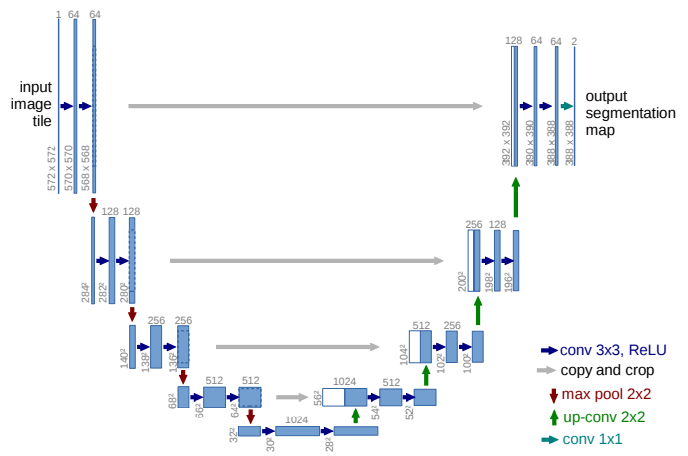
\includegraphics{./figures/chapter02_method/ronneberger1.png}
        \centering
        \caption {本論文主要研究的 U-Net 架構}
        \label{ronneberger1}
    \end{minipage}
    \hfil
\end{figure}

\subsection{濾波處理}
在頻譜域下的深度學習模型~\cite{hennequin2020spleeter,stoter20182018}通常會再採取濾波方法以增幅預測效果,且不增加太多預測時間(latency),首先定義下文會用到的符號。
\begin{itemize}
    \item $x(n)\in\mathbb{R}^2$ 表示混音軌(mixture stem)的時間序列
    \subitem $x(n)=s_{\textup{V}}{(n)} + s_{\textup{A}}{(n)} = \sum_{i\in\textup{I}}{s_i{(n)}}$
    \subitem $\textup{I} := \{\textup{V,A}\}$, $\textup{V}$: vocals主唱, $\textup{A}$: accompaniment伴奏
    \subitem $\hat{s_i}{(n)}$: 預測音軌的時間序列
    \item short-time Fourier transform (STFT) domain
    \subitem $X(m,f)\in\mathbb{C}^2$: 混音軌, $S_i(m,f)$: 來源分軌$_i$, $\hat{S_i}{(m,f)}$: 預測分軌$_i$
    \subitem $m$ 代表 frame;$f$ 代表 frequency bin
    \subitem $\vert\ast\vert$: STFT 的 magnitude, $\angle \ast$: STFT 的 phase
\end{itemize}

\subsubsection{Ratio Mask Filter}
% https://hal.inria.fr/hal-02293689/document
Ratio mask filtering 是一種直觀且簡單的作法,許多頻譜預測的方法~\cite{bao_abdulla_2018,stoter20182018}會再使用此,作為最後輸出訊號的遮罩,並且,可以此為基礎做另外衍伸。
\begin{equation*}
    \hat{S_i}{(m,f)} = \vert S_i(m,f)^E\vert (\sum_{j\in\textup{I}}\vert S_j(m,f)\vert^E)^{-1}X(m,f)
\end{equation*}
$E$ 代表 separation exponent,對於各種不同模型可以調整 ratio 以最佳化。
圖\ref{oracle_filtering1}與圖\ref{oracle_filtering2}\footnote{\url{https://colab.research.google.com/drive/1Zo6iSPIi6SjOAL7wg8yzVWkS9mjLgjI-?usp=sharing}}為實際 ratio mask 對主唱軌預測結果的遮罩與頻譜圖。

\begin{figure}[htbp]
    \hfil
    \begin{minipage}[t]{0.45\textwidth}
        \centering
        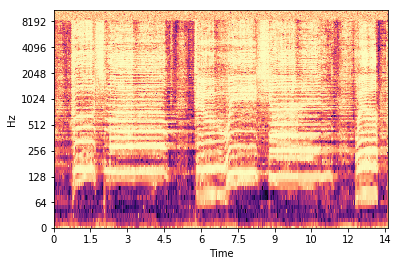
\includegraphics[width=\textwidth]{./figures/chapter02_method/oracle_filtering1.png}
        \caption {預測主唱軌的 ratio mask}
        \label{oracle_filtering1}
    \end{minipage}
    \begin{minipage}[t]{0.45\textwidth}
        \centering
        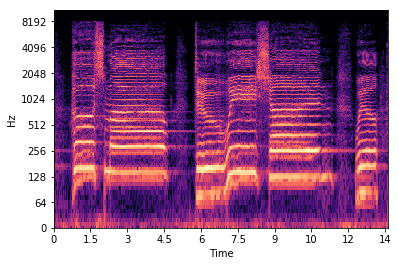
\includegraphics[width=\textwidth]{./figures/chapter02_method/oracle_filtering2.png}
        \caption {經過 ratio mask 濾過的主唱軌頻譜}
        \label{oracle_filtering2}
    \end{minipage}
    \hfil
\end{figure}

\subsubsection{Wiener Filter}
Wiener filter 是一種古老的訊號學技術,由 Wiener~\cite{wiener1949extrapolation} 提出。在此,假設 $s_\textup{V}{(n)}$ 與 $s_\textup{A}{(n)}$ 為廣義平穩不相關隨機序列,其功率譜密度分別是 $P_{s_\textup{V}}{(\omega)}$ 與 $P_{s_\textup{A}}{(\omega)}$ ,功率譜相加的式子:
\begin{equation*}
    P_{x}{(\omega)} = P_{s_\textup{V}}{(\omega)} + P_{s_\textup{A}}{(\omega)}
\end{equation*}
% file:///C:/Users/hp/Documents/MIR_Lab/report/21Oct2020_report/21Oct2020_report.pdf
基於訊號的統計特性,為了最大化其中一個訊號 $s_i{(n)}$,其解可由最小均方誤差 $ \textup{E}[(x(n)-s_{j}{(n)})^2] = \min$ 得出,簡易的 Wiener filter 可以理解為:
\begin{equation*}
    H_\textup{V}{(\omega)} = \frac{P_{s_\textup{V}}{(\omega)}{}}{P_{s_\textup{V}}{(\omega)} + P_{s_\textup{A}}{(\omega)}}
\end{equation*}
\begin{equation*}
    H_\textup{A}{(\omega)} = \frac{P_{s_\textup{A}}{(\omega)}}{P_{s_\textup{V}}{(\omega)} + P_{s_\textup{A}}{(\omega)}}
\end{equation*}

\subsubsection{頻譜刪減法}
在語音辨識系統中,使用理想的訓練語料訓練出一個聲學模型(acoustic model),這些訓練語料通常極為乾淨,然而實際應用中則不是理想環境,因此造成與訓練的模型無法完美吻合,導致辨識準確度下降。在辨識前,語音加強為一個重要步驟,希望能在辨識前,盡量減少環境雜訊對語音信號的影響,進而提升辨識率,頻譜刪減法~\cite{boll1979suppression}為其中一種語音加強演算法。
基於的假設:
\begin{itemize}
    \item 雜訊與原訊號不相干(uncorrelated)
    \item 雜訊與原訊號皆為 stationary
\end{itemize}
假設欲得到的加強訊號為 $x(n)$ 、包含雜訊的語音訊號為 $y(n)$ 且雜訊為 $r(n)$ 則:
\begin{equation*}
	\|X(\omega)\|^2=\left\{\begin{matrix}\|Y(\omega)\|^2-\|R(\omega)\|^2,\ \ \ if\ \ \|Y(\omega)\|^2-\|R(\omega)\|^2 > 0
\\ 
0,\ otherwise
\end{matrix}\right.
\end{equation*}


\subsection{深度神經模型 U-Net}
本節介紹目前開源的兩大歌聲分離模型,分別使用 U-Net 在頻域與時域中預測分離的訊號。

\subsubsection{Spleeter}
Spleeter~\cite{hennequin2020spleeter} 遵照了 Laure Prétet ~\cite{pretet2019singing}的訓練驗證方法,實現了 Jansson~\cite{jansson2017singing} 等人於2017年提出的 Deep U-Net 卷積模型(圖\ref{spleeter1}),基於聲音的頻譜圖,開源其程式碼~\footnote{\url{https://github.com/deezer/spleeter}}且在聲音訊號分離領域中取得優異的表現。

\begin{figure}[htbp]
    \hfil
    \begin{minipage}[t]{0.55\textwidth}
        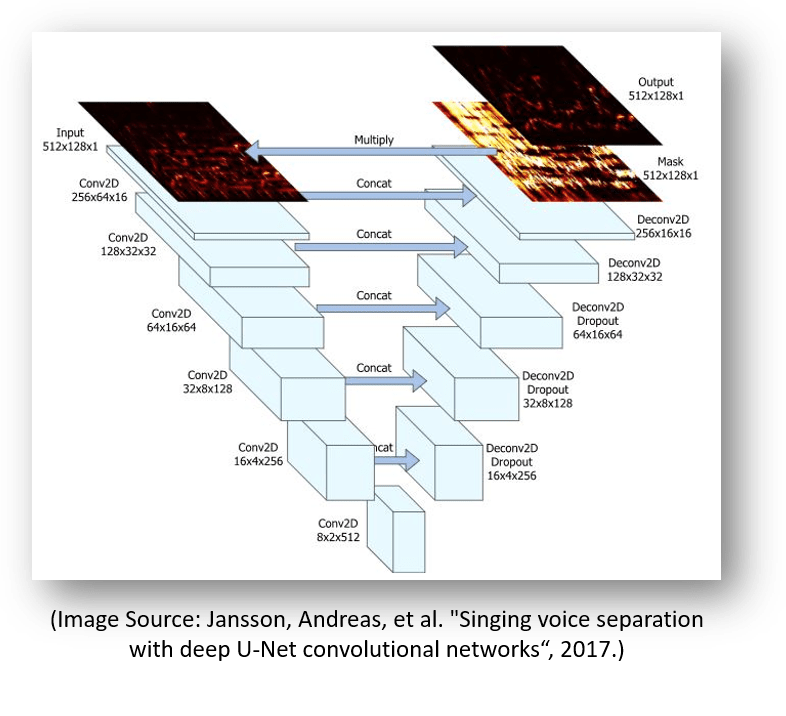
\includegraphics[width=\textwidth]{./figures/chapter02_method/spleeter1.png}
        \caption {Jansson 提出的 deep U-Net convolutional network}
        \label{spleeter1}
    \end{minipage}
    \hfil
\end{figure}

\subsubsection{Demucs}
Demucs~\cite{defossez2019music} FaceBook 基於 wave-u-net~\cite{stoller2018wave} 提出的弱監督訓練模型(圖\ref{demucs1}與圖\ref{demucs2})
\begin{figure}[htbp]
    \hfil
    \begin{minipage}[t]{0.45\textwidth}
        \centering
        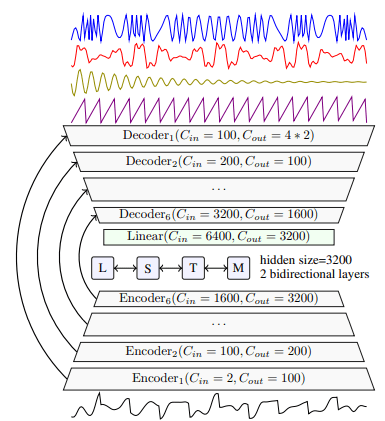
\includegraphics[width=\textwidth]{./figures/chapter02_method/demucs1.png}
        \caption {Demucs 的完整架構}
        \label{demucs1}
    \end{minipage}
    \begin{minipage}[t]{0.45\textwidth}
        \centering
        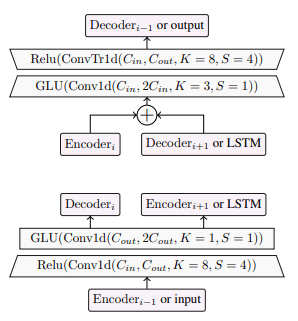
\includegraphics[width=\textwidth]{./figures/chapter02_method/demucs2.png}
        \caption {Encoder 與 decoder 細節}
        \label{demucs2}
    \end{minipage}
    \hfil
\end{figure}
在 wave-u-net 之上,於 encoder 與 decoder 加上了 GLU 的激活函數,也對 biLSTM 增加了更多通道以改進效果。在時域的訊號分離模型中,獲得很大的效能改進,並且也開源其程式碼\footnote{\url{https://github.com/facebookresearch/demucs}},對歌聲分離領域有很大的貢獻。

\subsection{注意力模型}
關於注意力模型(attention-based model),必須先談其起源,seq2seq模型的論文自2014年被發表~\cite{vaswani2017attention}以來,使機器在自然語言翻譯領域中取得很好的效果,seq2seq模型基本可以分為兩大部分 encoder 與 decoder,前者會將輸入語句編碼成類向量以表示初始狀態,後者則是使用該類向量預測下一字詞,產生新的文字內容。值得一提的是,輸入給定語句取得翻譯時,並不能觀察期中間產物的向量。

seq2seq模型看似強大,但也有個不可忽視的問題,當模型接受最後一個狀態的語句輸出作為 encoder 的輸入,產生其向量狀態時,RNN模型會有機率忘記太遠的資訊,即使加上LSTM~\cite{gers1999learning}或GLU仍無法妥善解決。此時,注意力模型就起到一個重要的作用,其度量了相似性。若當前的輸入語句與狀態向量越類似,那當前輸入的權重就越大。接下來會以台大李宏毅\footnote{\url{https://speech.ee.ntu.edu.tw/~tlkagk/}}老師的投影片為輔助,稍微解釋機器取得權重的方法(圖\ref{attention-based_model1}),decoder 在計算前會有一組模型參數 $z^0$,會與每個隱狀態 $h^i$ 進行匹配的運算,計算 $z^0$ 與 $h^i$ 的相似度最後得到注意價值度(attention score)$\alpha_0^i$,
\begin{figure}[htbp]
    \hfil
    \begin{minipage}[t]{0.45\textwidth}
        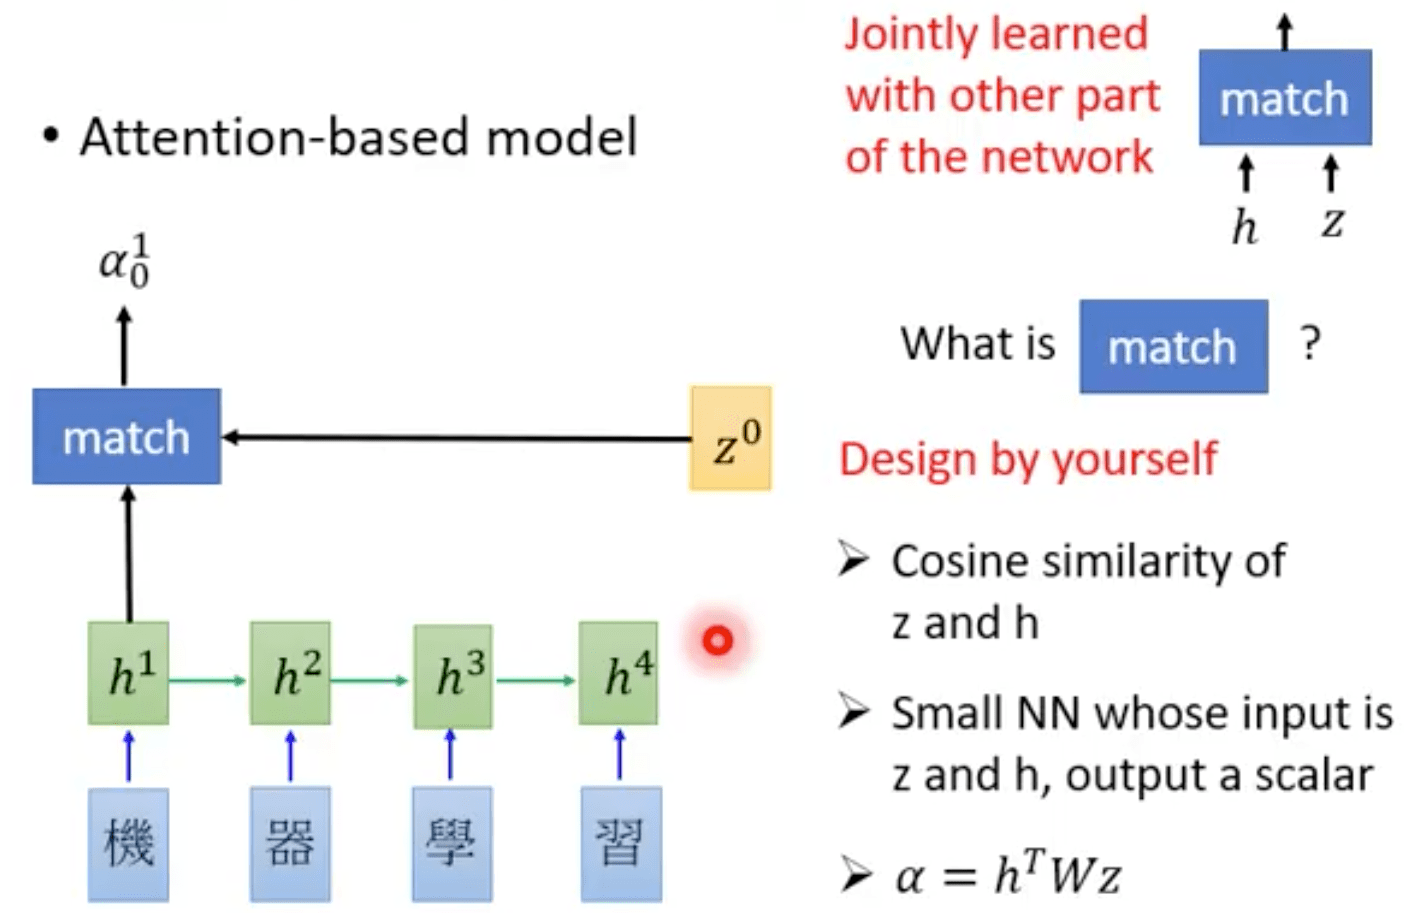
\includegraphics[width=\textwidth]{./figures/chapter02_method/attention-based_model1.png}
        \caption {注意力價值度的計算}
        \label{attention-based_model1}
    \end{minipage}
    \hfil
\end{figure}
得到了 $\alpha_0^i, i\in\{1,2,3,4\}$ 後,取 softmax 轉換成各自機率 $\hat{\alpha}_0^i, i\in\{1,2,3,4\}$,得到注意價值的機率分布,再以此作為隱狀態 $h^i$ 的加權得到 $c^0$(圖\ref{attention-based_model2}),最後給 decoder 進行解碼。 
\begin{figure}[htbp]
    \hfil
    \begin{minipage}[t]{0.45\textwidth}
        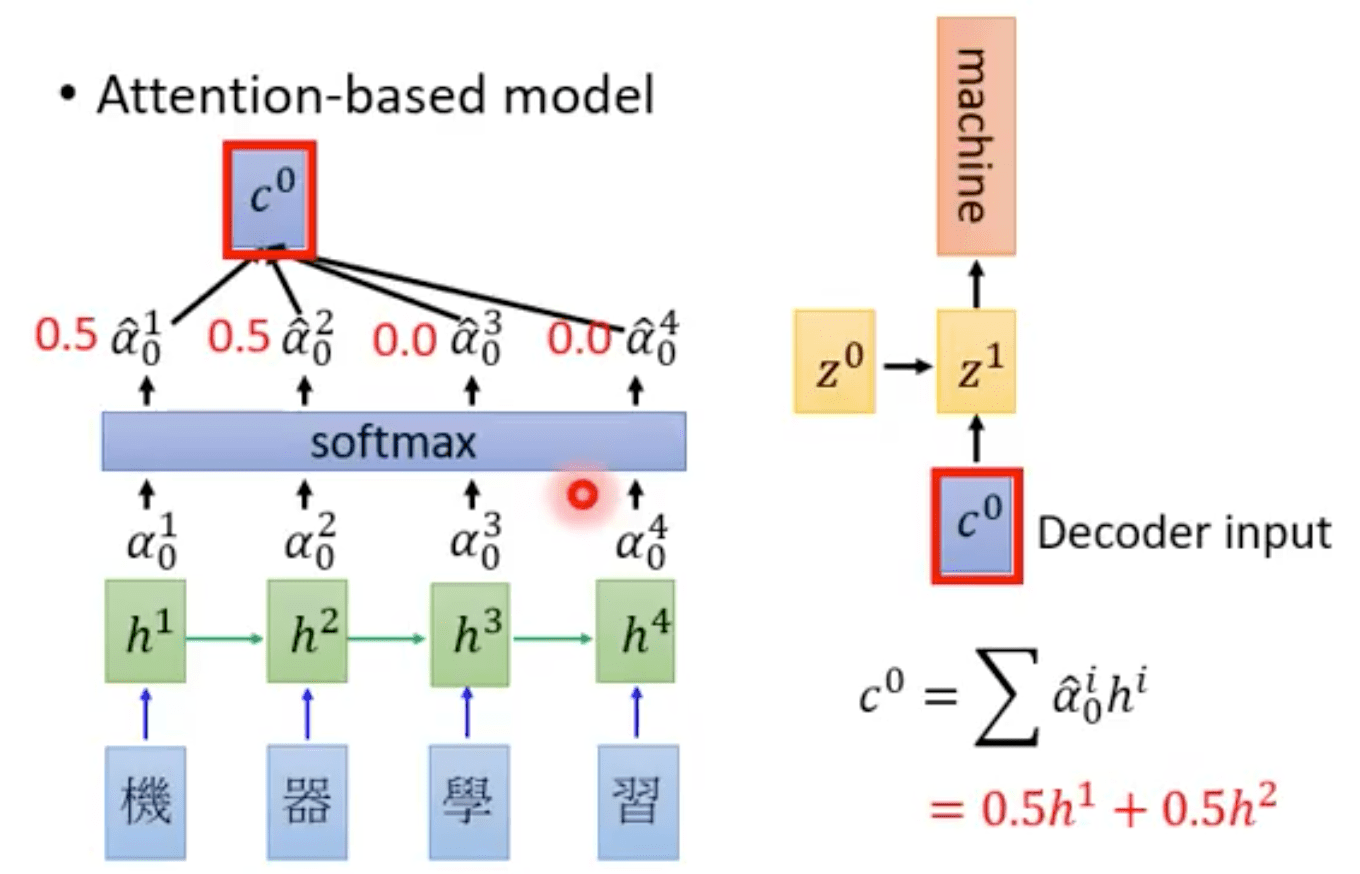
\includegraphics[width=\textwidth]{./figures/chapter02_method/attention-based_model2.png}
        \caption {使用注意力價值度計算新的隱狀態}
        \label{attention-based_model2}
    \end{minipage}
    \hfil
\end{figure}

這邊已經稍微介紹注意力模型的大致做法,接下來會講到其各自不同的實現方法。

\subsubsection{Self-attention}
Y. Liu 等人的研究中~\cite{liu2020voice},將原本在單一維度上使用的 self-attention 改成在雙維度上使用,以利頻譜在 U-Net 上的預測效果,原文指出:相同吉他和弦可能每 10 秒重複一次,對區域性的 CNN filter 來說太長,以致於在 Dense-UNet 中無法抓到這樣的聲音重複資訊;即使使用 BLSTM RNN 進行增強,MMDenseLSTM 仍無法處理跳躍性的聲音重複資訊,因為它只能著重在時間較近的記憶資訊。使用 self-attention 可以注意全局上所有位置的相同序列,並計算區域位置上相同序列的響應值給模型,此方法已經在機器翻譯與圖片生成\footnote{\url{https://github.com/brain-research/self-attention-gan}}領域中獲得採用~\cite{vaswani2017attention,zhang2019self},在改造雙維度上 self-attention 架構上,需要著重頻譜於時間維度上的資訊,期望可以找出音樂訊號中的規律,見圖\ref{self-attention1} 可以看到 self-attention 架構如何應用應用在歌聲分離之上。
\begin{figure}[htbp]
    \hfil
    \begin{minipage}[t]{0.80\textwidth}
        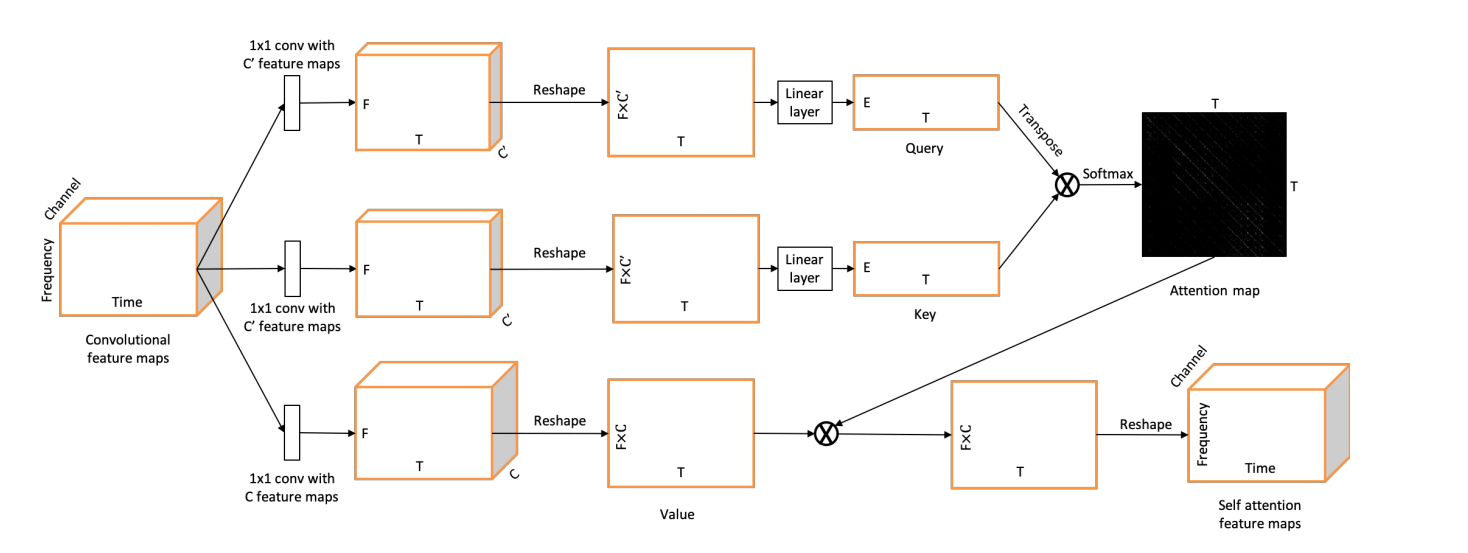
\includegraphics[width=\textwidth]{./figures/chapter02_method/self-attention1.png}
        \caption {Liu 提出的 self-attention 架構}
        \label{self-attention1}
    \end{minipage}
    \hfil
\end{figure}
\begin{figure}[htbp]
    \hfil
    \begin{minipage}[t]{0.80\textwidth}
        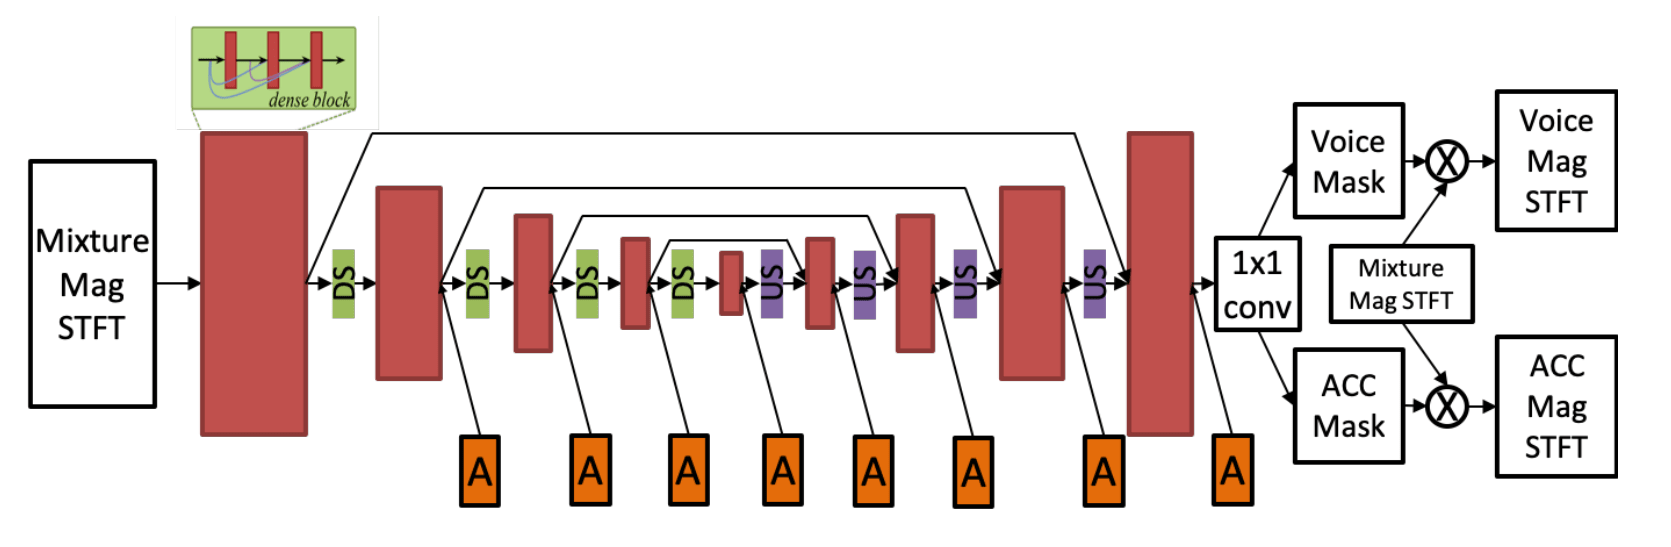
\includegraphics[width=\textwidth]{./figures/chapter02_method/self-attention2.png}
        \caption {Liu 應用在歌聲分離領域的模型架構}
        \label{self-attention2}
    \end{minipage}
    \hfil
\end{figure}

\subsubsection{Attention Gate}
「Attention u-net: Learning where to look for the pancreas」~\cite{oktay2018attention},U-Net 架構本身就很適合執行圖形切割的任務,但若要在醫學領域上可以妥善使用,必須克服少量的訓練資料但又達高精準度。Jetley 等人~\cite{jetley2018learn} 提出了一種 end-to-end\footnote{\url{https://www.itread01.com/content/1546712649.html}} 的 attention 架構「attention gate」,其被常用在自然景照分析與自然語言處理領域中。attention 被使用來彙集分類資訊,使影像分類領域可以更加準確,attention map 可強化有相關的區域,所以可以在各個指標性的資料集中鶴立雞群。
% https://jinglescode.github.io/2019/12/08/biomedical-image-segmentation-u-net-attention/
% https://www.itread01.com/content/1548179294.html#:~:text=%E7%9B%B8%E5%8F%8D%EF%BC%8CHard%20Attention%E6%98%AF%E4%B8%80%E5%80%8B,%E4%BC%B0%E8%A8%88%E6%A8%A1%E7%B5%84%E7%9A%84%E6%A2%AF%E5%BA%A6%E3%80%82
% https://kknews.cc/zh-tw/tech/ql559ao.html

Khened~\cite{khened2019fully} 與 Roth~\cite{roth2018spatial} 等人為了提升影像分割領域效能,需要倚靠額外的區域物件偵測模型隨後幫助圖形分割,研究後發現,在 U-Net 加上 attention gate 可以有效完成這件事,且不增加太多運算時間。在 U-Net 的並接運算(concatenation)之前,先合成全域有相關的激活值,這就是 attention gate (圖\ref{attention_gate1})的實現過程。
\begin{figure}[htbp]
    \hfil
    \begin{minipage}[t]{0.8\textwidth}
        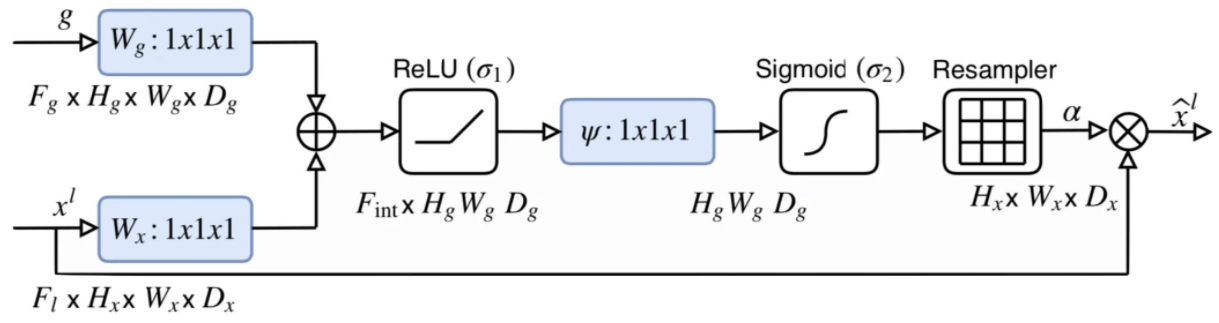
\includegraphics[width=\textwidth]{./figures/chapter02_method/attention_gate1.png}
        \caption {attention gate 架構}
        \label{attention_gate1}
    \end{minipage}
    \hfil
\end{figure}


\section{模型壓縮方法}
% 模型壓縮的東西~\cite{buciluǎ2006model}
雖然目前的硬體設備隨著摩爾定律越來越強,但人們也對低功耗的需求也與日俱增,套用在端點裝置如:手機、工廠監控晶片或是配置低的筆記型電腦。模型剪枝不只探討縮小也研究更快的執行,可以在實時的狀態下使用,如此一來可以更加貼近人們的生活。
% https://zhuanlan.zhihu.com/p/138059904


\subsection{模型剪枝}
本節探討模型剪枝(model pruning),模型壓縮的一種方法。下文探討的 MobileNets~\cite{howard2017mobilenets} ,其模型著重在圖形辨識領域之上,將傳統的卷積神經網路(CNN)改造,使之運算量大幅下降,這雖將模型裡訓練的參數大幅降低,可能導致效果便差,但既有 U-Net 足夠複雜的情況下,經過調整是有妥協空間的,接下來的子節會一一加以探討。

\subsubsection{深度可分卷積}
深度可分卷積(depth-wise separable convolution)是一種對普通卷積參數削減的方法,在 Chollet~\cite{chollet2017xception} 等人所提出的 xception 使用後被廣為人知,其採用深度可分卷積替換 inception v3 中的普通卷積,原作者的初衷是使 inception v3 架構更寬,但又不讓網路參數提升。Google 於 2017 提出的 MobileNet~\cite{howard2017mobilenets} 模型,欲解決巨大網路模型的瓶頸—卷積,在不降太多效能的情況下,使用深度可分卷積盡量減少原始卷積的計算量,將模型可以套用在手機或是攜帶裝置之上。

探討深度可分卷積與一般卷積的差異,運算量是非常值得關注的,為了方便解說,先定義一些使用到的參數:
\begin{itemize}
    \item 輸入資料 $F$
    \subitem 長 $=$ 寬 $=D_F$;高 $=M$
    \item 輸出資料 $G$
    \subitem 長 $=$ 寬 $=D_G$;高 $=N$
    \item 卷積 Kernel $K$
    \subitem 長 $=$ 寬 $=D_K$;高 $=M$;卷積數量 $=N$
    \subitem 卷積大小 $D_K \times D_K \times M \times N$
\end{itemize}
普通卷積在計算計算輸出資料 $G$ 的情況:
\begin{itemize}
    \item $G_{k,l,n}=\sum_{i,j,m}K_{i,j,m}\cdot F_{k+i-1,l+j-1,m}$
    \item 總運算量 $D_K \times D_K \times M \times N \times D_F \times D_F$
\end{itemize}
深度可分卷積在計算輸出資料 $\hat{G}$ 的情況:
\begin{itemize}
    \item $\hat{G}_{k,l,n}=\sum_{i,j}\hat{K}_{i,j,m}\cdot F_{k+i-1,l+j-1,m}$
    \item 總運算量 $D_K \times D_K \times M \times D_F \times D_F + M \times N \times D_F \times D_F$
\end{itemize}
其減少的運算量:
\begin{equation*}
\begin{split}
    \frac{\textup{Depthwise Separable Conv.}}{\textup{Normal Conv.}} \\
    = \frac{D_K \times D_K \times M \times D_F \times D_F + M \times N \times D_F \times D_F}{D_K \times D_K \times M \times N \times D_F \times D_F} \\
    = \frac{1}{N} + \frac{1}{D_K^2} &
\end{split}
\end{equation*}

舉例來說\footnote{\url{https://towardsdatascience.com/a-basic-introduction-to-separable-convolutions-b99ec3102728}
},輸入為一個$12\times 12\times 3$的圖,使用一個 $5\times5$ 二維卷積(no padding 與 1 stride),input(12x12) $\rightarrow$ conv(5x5) $\rightarrow$ output(8x8),普通卷積需要 1228800  運算量(圖\ref{depthwise_separable_conv1});深度可分卷積需要 53952 運算量(圖\ref{depthwise_separable_conv2})。縮小比值:0.043。

\begin{figure}[htbp]
    \hfil
    \begin{minipage}[t]{0.60\textwidth}
        \centering
        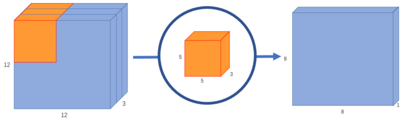
\includegraphics[width=\textwidth]{./figures/chapter02_method/depthwise_separable_conv1.png}
    \end{minipage}
    \caption {普通卷積的運算:需要 $256\times((3\times5\times5)\times(8\times8))=1228800$ 運算量}
    \label{depthwise_separable_conv1}
    \hfil
\end{figure}

\begin{figure}[htbp]
    \hfil
    \begin{minipage}[t]{1.0\textwidth}
        \centering
        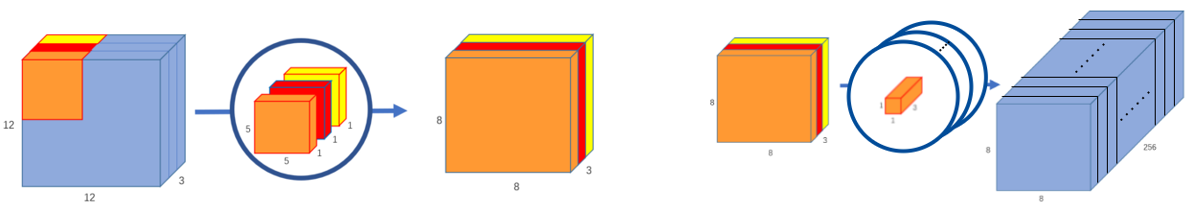
\includegraphics[width=\textwidth]{./figures/chapter02_method/depthwise_separable_conv2.png}
        \caption {深度可分卷積的運算:需要 $(3\times5\times5)\times(8\times8)+256\times((3\times1\times1)\times(8\times8))=53952$ 運算量}
        \label{depthwise_separable_conv2}
    \end{minipage}
    \hfil
\end{figure}


\subsubsection{Inverted Residuals 與 Linear Bottlenecks}
在訓練卷積神經網路模型時,比如本論文探討的 U-Net baseline,經常是層層堆疊,且對於每層的輸出,為了保留其最有用的資訊「manifold of interest」,會將其嵌入至一個低維度的子空間進行訓練。針對深度可分卷積架構,要如何在輕量化網路參數又不喪失太多資訊,MobileNet V2~\cite{sandler2018mobilenetv2} 提出的做法(圖\ref{inverted_residuals1}):
\begin{itemize}
    \item[1.] 作 depthwise separable convolution 前,先作一層 pointwise convolution 提升輸出維度(此作法稱為「linear bottleneck layer」)
    \item[2.] 最後輸出前使用「linear activation function」以避免過度的資訊過濾
\end{itemize}
\begin{figure}[htbp]
    \hfil
    \begin{minipage}[t]{0.65\textwidth}
        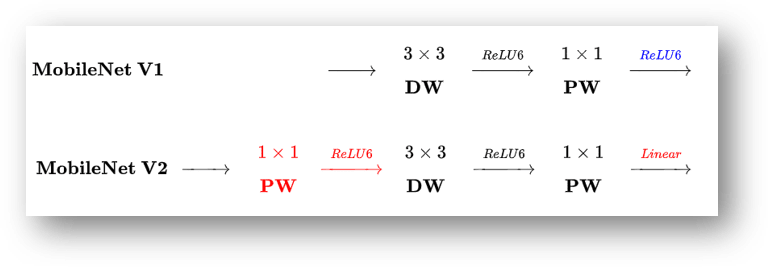
\includegraphics[width=\textwidth]{./figures/chapter02_method/inverted_residuals1.png}
        \caption {MobileNet V2 對深度可分卷積做出的改進}
        \label{inverted_residuals1}
    \end{minipage}
    \hfil
\end{figure}
而如此的作法極相似於 Resnet~\cite{he2016deep} 中被廣泛使用的 residual block,(圖\ref{inverted_residuals2}-(a))在過去會將 channel 先壓縮在進行卷積, shortcut 連接兩個較大的 channel 以傳遞資訊,(圖\ref{inverted_residuals2}-(b))在 MobileNet V2 中,shortcut 連接兩個較小的 channel,是為了將經過「linear bottleneck layer」中有用的資訊「manifold of interest」嵌入至低維度的子空間。
\begin{figure}[htbp]
    \hfil
    \begin{minipage}[t]{0.65\textwidth}
        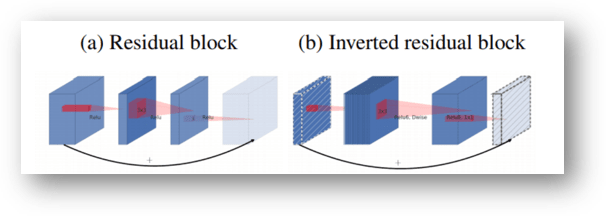
\includegraphics[width=\textwidth]{./figures/chapter02_method/inverted_residuals2.png}
        \caption {Inverted residuals}
        \label{inverted_residuals2}
    \end{minipage}
    \hfil
\end{figure}


\subsection{模型量化}
模型量化由模型與量化兩詞組成。在深度學習領域下,模型指的是神經網路。而量化是指降低精準度,通常以定點(通常為「int8」)近似浮點數模型,從而降低模型儲存於記憶體的消耗,也有機會可以加速模型在預測的速度,下式與圖 表示基本的線性量化方法。

\begin{itemize}
    \item 量化(Quantize)
    \subitem $x_\textup{int} = \textup{round}(\frac{x}{\Delta})+z$
    \subitem $x_Q = \textup{clamp}(0,N_\textup{levels}-1,x_\textup{int})$
    \item 反量化(De-quantize)
    \subitem $x_\textup{float} = (x_Q-z)\times\Delta$
\end{itemize}
\begin{figure}[htbp]
    \hfil
    \begin{minipage}[t]{0.4\textwidth}
        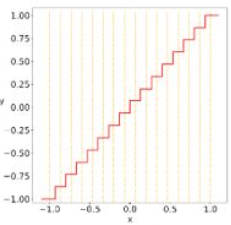
\includegraphics[width=\textwidth]{./figures/chapter02_method/quantization1.png}
        \caption {基礎線性量化}
        \label{quantization1}
    \end{minipage}
    \hfil
\end{figure}

\subsubsection{Quantized Neural Networks PACKage}
QNNPACK (quantized neural networks package)~\cite{dukhan2018qnnpack,wu2019machine} 是 Marat Dukhan 開發專用於量化神經網路計算的 Python 套件,其卓越的性能,在2019年一經開源\footnote{\url{https://github.com/pytorch/QNNPACK}}就擊敗了幾乎當時全部已公開的加速演算法。接下來本節會參考此\footnote{\url{https://jackwish.net/2019/reveal-qnnpack-implementation.html}}文章以描述 QNNPACK 的實現方法。在矩陣乘法優化階段,是針對輸出矩陣的劃分,拆分成圖\ref{qnnpack1} 的 $MR \times NR$ 小塊,再做矩陣的乘法,提高指令集的使用度。
\begin{figure}[htbp]
    \hfil
    \begin{minipage}[t]{0.8\textwidth}
        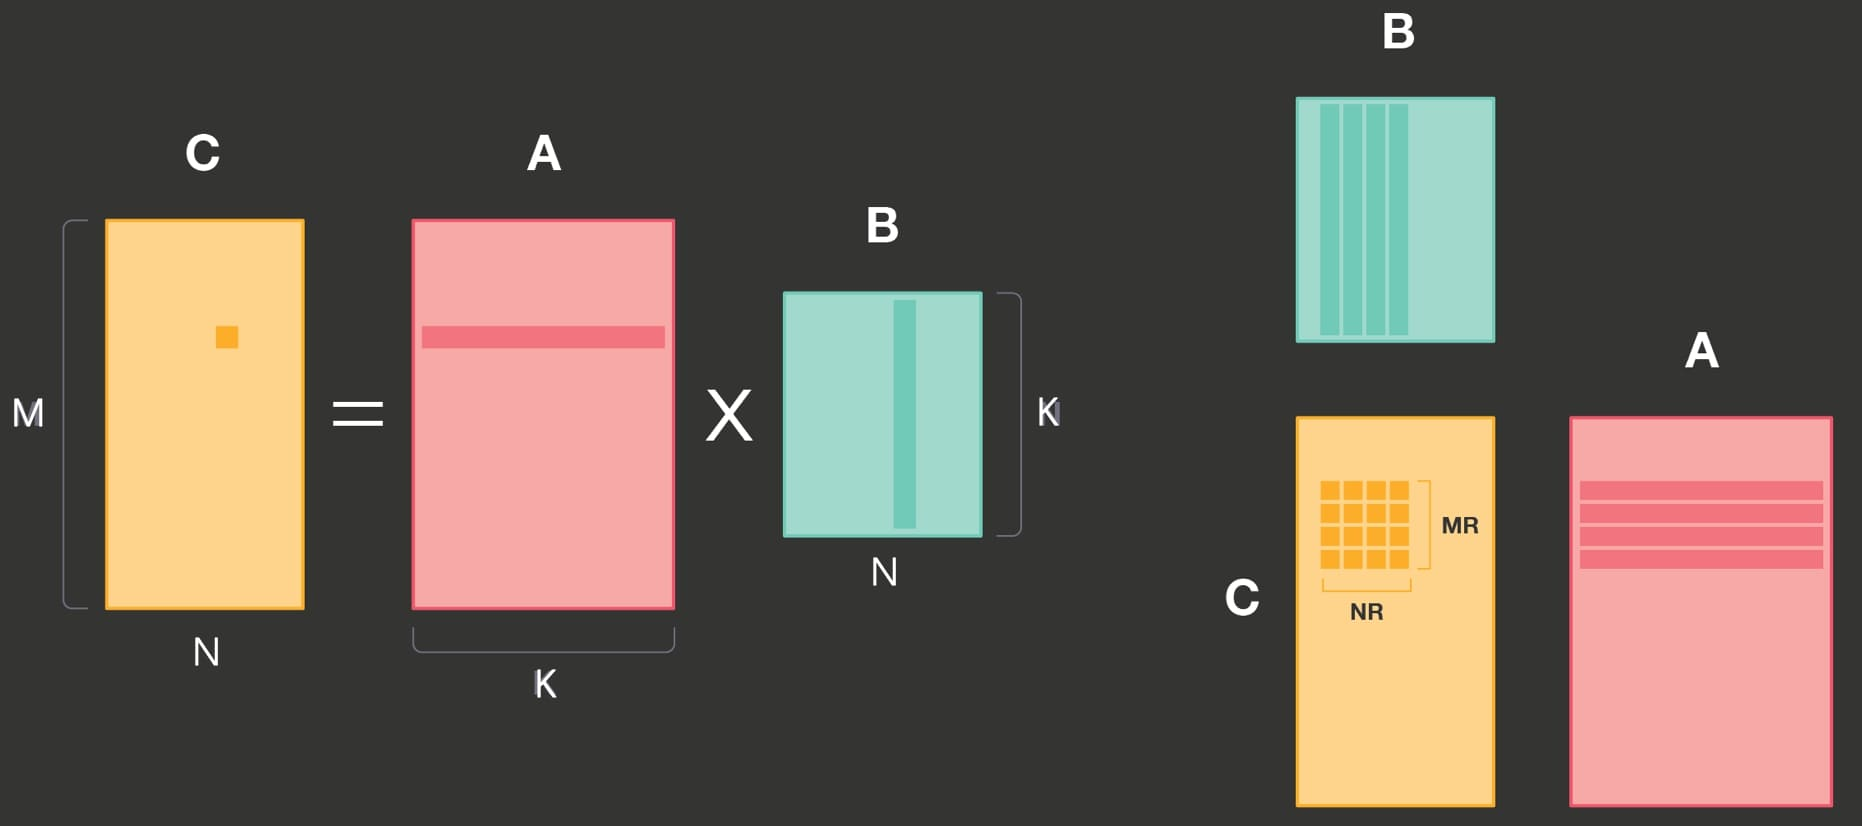
\includegraphics[width=\textwidth]{./figures/chapter02_method/qnnpack1.jpg}
        \caption {QNNPACK 的矩陣乘法優化}
        \label{qnnpack1}
    \end{minipage}
    \hfil
\end{figure}
矩陣乘法的優化中,QNNPACK 也改變實現矩陣乘法的底層以提高了 armv7 與 arm64 指令集的使用度,計算過程妥善使用 L1 cache 的優勢,亦對記憶體進行重新組織(repacking),以改進高速緩存的命中率。
\chapter{資料集簡介}
接下來的章節會介紹本論文實驗的過程中,所使用到的音樂資料集,其中除了有網路上對於教學公開的資料集,也有台大MIRLAB實驗室合作對象所提供的資料集,這些資料都極其寶貴,謝謝這些人的付出,對人工智慧在音樂分析領域中做出了極大的貢獻。公開的資料集包含:MUSDB18~\cite{rafii2017musdb18,musdb18}、DSD100~\cite{SiSEC16}、MedleyDB~\cite{bittner2014medleydb}、iKala~\cite{chan2015vocal};非公開的資料集包含:Ke(捷奏錄音室-柯老師)、其餘資料(台大MIRLAB蒐集而成)。接下來會細述這些資料的取得方法,與其內容音檔概述,若要知道粗略的比較可從表\ref{dataset_bref}中取得資訊。另外本章也會概述模型評估基準 Museval~\cite{stoter20182018},其已被打包成 Python 套件方便人工智慧的發展。

\begin{table}[h!]
\centering
\resizebox{\linewidth}{!}{
\begin{tabular}{|r|c|c|c|c|c|c|}
\hline
 & iKala & DSD100 & MedleyDB & MUSDB18 & Ke & 獨立蒐集 \\ \hline
提出年份(公開) & 2015 & 2015 & 2014 & 2017 & N/A & N/A \\ \hline
歌曲資料數 & 306 & 100 & 122 & 150 & 727 & 413 \\ \hline
歌曲時長 & 30秒 & 251±60秒 & 206±121秒 & 236±95秒 & 3~4分鐘 & 3~4分鐘 \\ \hline
總時間長度 & 2小時 & 7小時 & 7.2小時 & 10小時 & 54小時 & 29小時 \\ \hline
完整歌曲/立體聲 & 否/無 & 是/有 & 是/有 & 是/有 & 是/有 & 是/有 \\ \hline
有人聲的歌曲比例 & 100% & 100% & 57% & 100% & 100% & 100% \\ \hline
歌曲分軌數 & 2 & 4 & 1~26 & 4 & 6 & 4 \\ \hline
樂器種類數 & 2 & 4 & 82 & 4 & 6 & 4 \\ \hline
\end{tabular}
}
\caption{資料集概述}
\label{dataset_bref}
\end{table}

\section{MusDB18}
MUSDB18資料集~\cite{rafii2017musdb18,musdb18}\footnote{\url{https://sigsep.github.io/datasets/musdb.html}}由150首不同曲風的雙聲道歌曲組成,其聲音以 44.1khz 編碼,總時長約10小時,聲音分離比賽 2018 Signal Separation Evaluation Campaign~\cite{stoter20182018} 以此資料集為基礎進行,每首歌除了有混音軌(mixture stem),皆包含四個分部:主唱(vocals stem)、鼓 (drums stem)、貝斯(bass stem)、其他(other stem)等4軌。資料集已由官方分成訓練資料和測試資料兩類,其訓練資料共100首,測試資料共50首。資料的來源包含: DSD100 的100首、 MedleyDB 的46首、 Native Instruments 的2首、加拿大樂隊 The Easton Ellises\footnote{\url{https://g.co/kgs/Gqm6Vg}} 的2首。

\subsection{DSD100}
DSD100資料集~\cite{SiSEC16}\footnote{\url{https://sigsep.github.io/datasets/dsd100.html}}由100首不同曲風的雙聲道歌曲組成,聲音分離比賽 Signal Separation Evaluation Challenge 2016~\cite{liutkus20172016} 以此資料集為基礎進行,每首歌除了有混音軌(mixture stem),皆包含四個分部:主唱(vocals stem)、鼓 (drums stem)、貝斯(bass stem)、其他(other stem)等4軌。資料集已由官方分成訓練資料和測試資料兩類,其訓練資料共50首,測試資料共50首。資料的來源是從「'Mixing Secrets' Free Multitrack Download Library」\footnote{\url{https://www.cambridge-mt.com/ms/mtk/}}中汲取而成,特別感謝Mike Senior的允許使用也感謝他對此資料的維護。

\subsection{MedleyDB}
MedleyDB資料集~\cite{bittner2014medleydb}\footnote{\url{https://medleydb.weebly.com/}}由紐約大學音樂與音頻研究實驗室~\footnote{\url{https://steinhardt.nyu.edu/marl}}主導建立,共有196首(44.1kHz、16bit)的歌曲,資料集詳細註記每首歌曲的資訊:曲風、歌曲長度、作曲者、歌手性別等等,對每首歌曲以樂器為單位詳細記錄其分軌,一首歌曲可能會被分成數10軌不等,有助於研究不同歌曲造成差異的原因。圖 \ref{medleyDB_inst}和圖 \ref{medleyDB_genre} 為音軌和曲風的詳細資訊。

\begin{figure}[htbp]
    \centering
    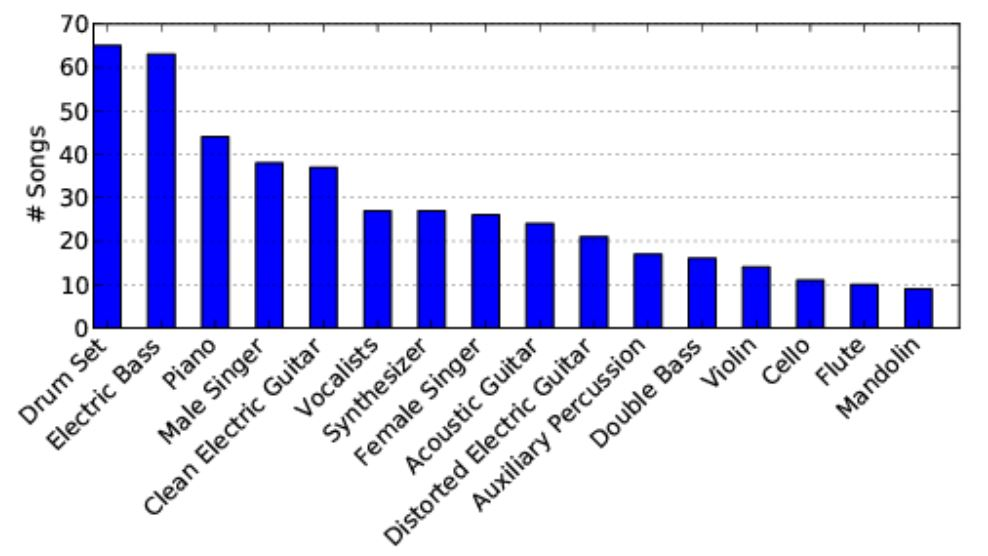
\includegraphics[width=0.6\textwidth]{./figures/chapter03_dataset/medleyDB_inst.jpg}
    \caption{MedleyDB音軌資訊}
    \label{medleyDB_inst}
\end{figure}
\begin{figure}[htbp]
    \centering
    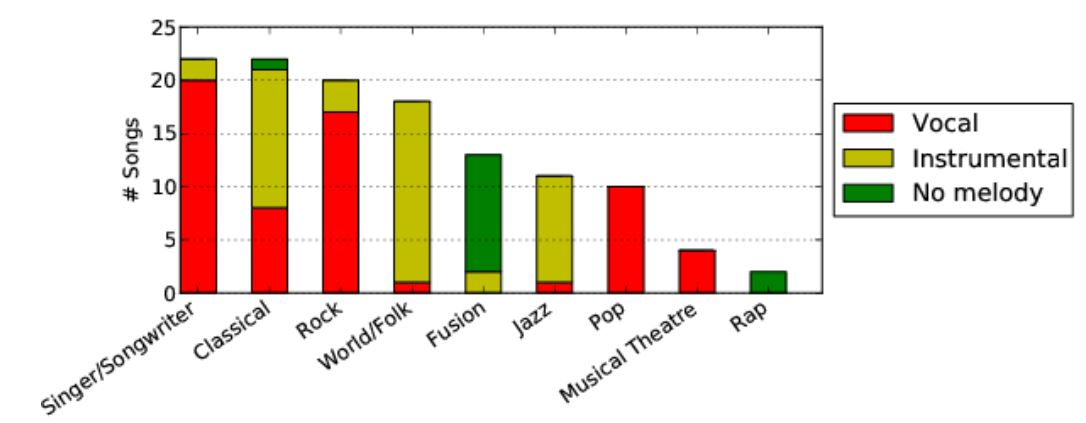
\includegraphics[width=0.8\textwidth]{./figures/chapter03_dataset/medleyDB_genre.jpg}
    \caption{MedleyDB曲風資訊}
    \label{medleyDB_genre}
\end{figure}

\subsection{Museval 模型測試指標}
% stoter2018museval,stoter20182018
在提及此測試指標之前,需先提到一個音樂分離比賽,也就是 2018 Signal Separation Evaluation Campaign~\cite{stoter20182018},其比賽除了透過MUSDB18資料集~\cite{rafii2017musdb18,musdb18}進行,另外提供了一個Python套件\footnote{\url{https://github.com/sigsep/sigsep-mus-eval}}稱為Museval~\cite{stoter2018museval},方便指標的計算與模型評估。此指標被多數音樂分離領域的研究中採用,其中有兩大開源實驗項目:Facebook 開發的 Demucs\footnote{\url{https://github.com/facebookresearch/demucs}} 、Deezer 開發的 Spleeter\footnote{\url{https://github.com/deezer/spleeter}},皆使用此評估開發中的模型優劣,目前可見的論文也都採用此,這極大地幫助實驗進行。套件目的在於評估分離模型分析的結果並輸出有效的 json 檔案,希望研究人員使用此評估輸出格式作為「共享分離結果」的標準,Museval 設計與 Musdb18 結合使用。


\section{iKala}
iKala資料集~\cite{chan2015vocal}\footnote{\url{http://mac.citi.sinica.edu.tw/ikala/}}是在MIR-1K資料集之後,由iKala、台大 MIRLAB 和中研院 MACLAB\footnote{\url{http://mac.citi.sinica.edu.tw/}} 共同建立的高品質分軌歌曲資料集,並且也是為數不多的中文歌曲資料集,其中資料是從206首歌曲中以30秒為單位並用44.1kHz進行採樣,最後取得252個片段,且每個片段都已經分軌為人聲和背景音樂資料,此外,iKala中的每首歌曲都有標記音高和歌詞出現的時間點,讓可以使用此資料集的研究領域更廣,表\ref{comp_mir_1k_with_ikala}為 MIR-1K 與 iKala 資料集的比較。

\begin{table}[h!]
\centering
\begin{tabular}{|r|c|c|}
\hline
\textbf{}                 & \textbf{MIR-1K} & \textbf{iKala} \\ \hline
Sample rate               & 16kHz           & 44.1kHz        \\ \hline
Singer quality            & Amateur         & Professional   \\ \hline
Clip duration             & 4-13s           & 30s            \\ \hline
Number of clips           & 1000            & 252            \\ \hline
Voice recorded separately & Yes             & Yes            \\ \hline
Pitch contour annotations & Yes             & Yes            \\ \hline
Voice type annotations    & Yes             & No             \\ \hline
Lyrics with speech        & Yes             & No             \\ \hline
Lyrics with timestamps    & No              & Yes            \\ \hline
Separate chorus and verse & No              & Yes            \\ \hline
Instrumental solo         & No              & Yes            \\ \hline
\end{tabular}
\caption{MIR-1K與iKala資料集的比較}
\label{comp_mir_1k_with_ikala}
\end{table}

\section{捷奏錄音室-柯老師}
資料集由本次研究合作的捷奏錄音室提供,捷奏錄音室是民國78年創立時,國內少數專業的大型錄音室。在此資料集中,總共有727首分軌歌曲,MIRLAB將歌曲資料經過處理後,最後依照一般歌曲的主要樂器分成6軌,分別為:主唱(vocals stem)、鼓 (drums stem)、貝斯(bass stem)、其他(other stem)、吉他(guitar stem)、電吉他(e-guitar stem)。此資料集的歌曲包含許多中文流行音樂、鄉村音樂,大量的歌曲資料有助於增加機器學習模型訓練效果。

\section{其餘資料收集}
MIRLAB的黃翔宇~\footnote{\url{hsiangyu.huang@mirlab.org}}透過目前現有的歌曲分離來源技術,對混音好地近年熱門流行歌曲進行分離,因此對應每個音軌並不是完全正確的。總共有413首歌曲,並將每首歌曲都分成4軌,主唱(vocals stem)、鼓 (drums stem)、貝斯(bass stem)、其他(other stem)。
\chapter{研究方法}
\section{問題定義}
使用深度學習在歌聲分離領域上,本論文採取監督式學習訓練,取音樂訊號的頻譜(spectrogram)後,對其做值域轉換成為模型訓練使用的特徵,模型的輸出應為主唱(vocals stem)與伴奏(accompaniment stem)的頻譜,現在主流的架構建立於 U-Net~\cite{ronneberger2015u,jansson2017singing,hennequin2020spleeter,defossez2019music} 之上,憑藉其在圖像分割領域卓越的表現,期許在頻譜圖也能有所突破。對於 U-Net 的輸出,是否能經過簡單的處理就能提高其預測質量也是一個值得探討的問題。另外,在實際部屬 U-Net 模型時有個不可漠視的問題,其龐大的架構不適合在行動裝置上與晶片上搭載,會面臨模型預測時間長與裝置記憶體不足的問題。本論文的研究建立在現有的 U-Net 模型架構上進行分析與改良,主要有:
\begin{itemize}
	\item[1.] 基於 ratio mask filter 與 Wiener filter 理論,善加利用現有的 U-Net 模型之預測頻譜圖,以提升輸出質量。
	\item[2.] 研究不同的 U-Net 架構,本篇會著重在注意力模型 attention gate 與 self-attention 的基礎上做延伸,設計一新的 U-Net 模型,並測試對於分離歌聲的效果。
	\item[3.] 基於先前頻譜刪減(spectral subtraction)~\cite{boll1979suppression} 的研究,探討其問題與設法提升其效果。
	\item[4.] U-Net 模型壓縮實驗,使用模型剪枝(model pruning)與模型量化(model quantization)來達成。
\end{itemize}

\section{實驗環境}
\begin{itemize}
    \item Server
    \subitem CPU:{\bf Intel(R) Xeon(R) Silver 4116 @ 2.10GHz}
    \subitem RAM:{\bf 314 GB}
    \subitem GPU:{\bf NVIDIA Quadro GV100 and NVIDIA TITAN RTX}
    \item Edge device
    \subitem Model name:{\bf Raspberry Pi 4 Model B}
    \subitem CPU:{\bf Quad core Cortex-A72 (ARM v8) 64-bit SoC @ 1.5GHz}
    \subitem RAM:{\bf 4GB}
    \subitem GPU:{\bf None}
\end{itemize}


\section{評量指標}
Vincent~\cite{vincent2006performance} 提出的指標評量以比較「原始聲音」與「預測聲音」的差距與量化,在本論文中,探討的是「原始音軌」與「U-Net 模型預測的音軌」。本篇使用的是 Python 套件 Museval~\cite{stoter2018museval}\footnote{\url{https://github.com/sigsep/sigsep-mus-eval}},一個以前述指標包裝而成的套件,由 SegSep\footnote{\url{https://sigsep.github.io/}} 團隊維護而成,並在 2018 signal separation evaluation campaign~\cite{stoter20182018} 中所採取,此領域的研究也以此做為評估指標,這些都代表著其重要程度,適合被本論文所採取。Museval 使用 Musdb18~\cite{rafii2017musdb18,musdb18} 的測試集做 Vincent 定義的指標,以該資料集中每一首歌每秒為單位,比較「原始聲音」與「預測聲音」的差距,並以 json 格式儲存後以便上傳至比賽單位,最後做整體評估~\cite{stoter20182018}時,在每首歌中的評量裡取其中位數作為該歌曲的得分,在該資料集中取其中位數作為該資料集的得分。Vincent 定義分離的訊號是由 4 個元素組成,等式如下:
\begin{equation*}
    \widehat{s_j}=s_\textup{target}+e_\textup{interf}+e_\textup{noise}+e_\textup{artif}
\end{equation*}
其中:
\begin{itemize}
    \item $s_\textup{target}$:目標來源的訊號(為目標音軌的原始聲音)
    \item $e_\textup{interf}$:表示其他來源訊號的干擾(為其他音軌參雜而導致的噪音)
    \item $e_\textup{noise}$:表示訊號中的雜訊
    \item $e_\textup{artif}$:額外產生的干擾(為 U-Net 在預測過程中產生的噪音)
\end{itemize}
Vincent 依照上面定義設計了 SDR、SIR 與 SAR 指標:
\begin{itemize}
    \item Source-to-Distortion Ratio(SDR):此指標為評量分離結果的總失真程度,當 SDR 值越高時,代表分離結果與實際訊號的總失真越低;反之,當 SDR 值越低時,代表總失真越高。
        \begin{equation*}
        SDR:=10\log_{10}\frac{\|s_\textup{target}\|^2}{\|e_\textup{interf}+e_\textup{noise}+e_\textup{artif}\|^2}
        \end{equation*}
    \item Source-to-Interferences Ratio(SIR):此指標為評量分離結果受其他來源干擾的程度,當 SIR 值越高時,代表分離結果受其他來源干擾越低;反之,當 SIR 值越低時,代表受其他來源干擾越高。
        \begin{equation*}
        SIR:=10\log_{10}\frac{\|s_\textup{target}\|^2}{\|e_\textup{interf}\|^2}
        \end{equation*}
    \item Sources-to-Artifacts Ratio(SAR):此指標評估模型預測時額外產生的干擾程度,當 SAR 值越高時,代表在分離結果中,額外產生的干擾程度越低;反之,當 SAR 值越低時,代表額外產生的干擾程度越高。
        \begin{equation*}
        SAR:=10\log_{10}\frac{\|s_\textup{target}+e_\textup{interf}+e_\textup{noise}\|^2}{\|e_\textup{artif}\|^2}
        \end{equation*}
\end{itemize}
基於上面指標的描述,也根據這篇問答\footnote{\href{https://dsp.stackexchange.com/questions/9610/snr-calculation-in-audio-reconstruction-and-what-is-an-acceptable-value}{Stackexchange Q\&A}},本輪文的研究可泛用在KTV產業界中,主要以提升伴奏質量為優先。可以注意的是,在必要的妥協下,可以捨去 SIR (伴奏中可以出現些許的主唱),專注提升 SAR (減少 U-Net 模型賦予的噪音),使 short-time-fourier-transform 的 window 越大可讓 SIR 提升而讓 SAR 下降。

\section{實驗設計與方法}
下文裡實驗中的模型,只使用 Musdb18 中的資料以訓練,以本文的實驗基準 U-Net 來說,使用所有的資料集進行完整訓練,大約需要14天,但若只使用 Musdb18 進行訓練,只需2天即可,另外 Demucs~\cite{defossez2019music} 的研究中,也有只使用 Musdb18 作為訓練的實驗,綜觀考量之下,本論文採取此做法以節省時間,但在最後挑出的最好模型,仍會進行一次完整資料集的訓練,確認模型效能。

\subsection{神經模型訓練設定}
\begin{itemize}
    \item Feature extraction
    \subitem Sample frequency:44.1 kHz
    \subitem Frame size:4096
    \subitem Step size:1024
    \subitem Feature (neural net input):$\log_e{1+\vert X\vert} $, $\vert X\vert$ stands magnitude of signal
    \subitem Cropping: Frequency bin(F)to 2048 and frame size(T) to 216
    \item Neural net training (PyTorch environment)
    \subitem Epoch:200
    \subitem Batch size:6
    \subitem Optimizer:Adam~\cite{kingma2014adam}
    \subitem Learning rate:0.0001
    \subitem Loss:smooth L1 loss\footnote{\url{https://pytorch.org/docs/stable/generated/torch.nn.SmoothL1Loss.html}}
    \subitem LR scheduler:reduce lr on plateau\footnote{\url{https://pytorch.org/docs/stable/optim.html}}
\end{itemize}
這邊採取的 smooth L1 loss 函數可以視為平滑版的 L1 loss 函數(圖\ref{xLxLoss1})。當預測值 $f(x_i)$ 與對應的正確值 $y_i$ 差異較小時(絕對差小於1),smooth L1 loss 函數其實是使用了 L2 Loss,使梯度不會太大;在差異大時,採取類 L1 loss 函數的方法,梯度穩定,不導致梯度爆炸。通常 smooth L1 loss 函數應用在大多數問題,亦在本論文的實驗中。

\begin{equation*}
    loss(x,y)=\frac{1}{n}\sum_{i=1}^{n}\left\{\begin{matrix}
        0.5 \times (y_i-f(x_i))^2,& \textup{if}\ \vert y_i-f(x_i)\vert < 1\\ 
        \vert y_i-f(x_i)\vert -0.5,& \textup{otherwise}
    \end{matrix}\right.
\end{equation*}

\begin{figure}[htbp]
    \hfil
    \begin{minipage}[t]{0.6\textwidth}
        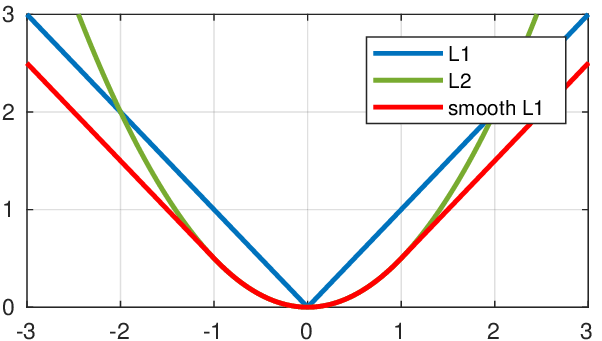
\includegraphics[width=\textwidth]{./figures/chapter04_experiment/xLxLoss1.png}
        \caption {Loss 函數比較圖}
        \label{xLxLoss1}
    \end{minipage}
    \hfil
\end{figure}

\subsection{濾波實驗}
本節說明濾波實驗的緣由。基於既有已訓練的 U-Net baseline 模型,採取適合的後處理也很重要,本論文主要探討 ratio mask filter 與 Wiener filter 作為後處理對模型預測的增幅。Python 套件 norbert~\cite{liutkus2019sigsep}\footnote{\url{https://github.com/sigsep/norbert}} 將此包裝,並在本實驗過程中使用。既有 U-Net 的輸出為頻譜域,要將其轉換為時間域,過去的方法是直接與混音軌的相位合併,再使用 iSTFT 轉回(圖\ref{Filter1}),本論文將 U-Net 的輸出頻譜轉換為一個濾波器,再對混音軌的 STFT 域做過濾(圖\ref{Filter2}),並在下章比對其效能。

\begin{figure}[htbp]
    \hfil
    \begin{minipage}[t]{0.8\textwidth}
        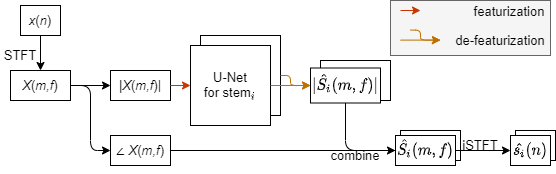
\includegraphics[width=\textwidth]{./figures/chapter04_experiment/Filter1.png}
        \caption {原始轉換方法}
        \label{Filter1}
    \end{minipage}
    \hfil
\end{figure}

\begin{figure}[htbp]
    \hfil
    \begin{minipage}[t]{0.8\textwidth}
        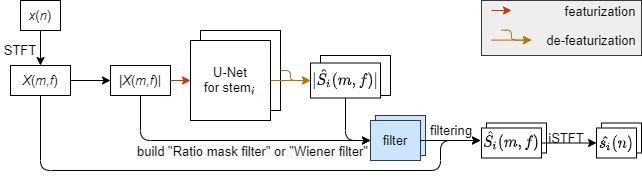
\includegraphics[width=\textwidth]{./figures/chapter04_experiment/Filter2.png}
        \caption {本論文轉換方法}
        \label{Filter2}
    \end{minipage}
    \hfil
\end{figure}

\subsubsection{頻譜刪減法}
在先前的實驗中,成功的將下式套用在歌聲分離領域:
\begin{equation}
	\|X(\omega)\|^2=\left\{\begin{matrix}\|Y(\omega)\|^2-\alpha\cdot\|R(\omega)\|^2,\ \ \ if\ \ \|Y(\omega)\|^2-\alpha\cdot\|R(\omega)\|^2 > 0
\\ 
0,\ otherwise
\end{matrix}\right.
\end{equation}
其中 $\alpha$ 控制刪減的幅度,在 U-Net 預測出主唱聲與伴奏頻譜以經頗為優越的情況下,以此演算法得到更佳的輸出,經數據證明,在 $\alpha=0.2$ 的時候,其效果有些許地增幅,數據會與本次實驗放在下一章做比較。
因此,將頻譜刪減法套用於歌聲分離領域是可行的,本論文將會著重在各個頻譜中,控制每個不同 frequency bin 在不同刪減的幅度 $\alpha$ 的情況下,是否可以得到更好的效果,本論文會以兩種方式對此探討。

第一種方式,最直覺的作法就是對"每個" frequency bin $f$ 窮舉所有的 $\alpha_f$,在一個給定的資料集下,找到對應最好的刪減幅度,但這會面臨到四個問題:frequency bin 太多(一個模型輸出的頻譜有 2048 個 frequency bin)、 $0\leq\alpha_f\leq1$ 之間的實數要如何枚舉、資料集大小的界定、窮舉所有 $\alpha_f$ 的可行性。在時間與現有機器的妥協下,本論文實驗以一種較為單純可行的設定進行:

\begin{itemize}
    \item[1.] frequency bin 太多(頻譜有 2048 個 frequency bin)
        \subitem 以 256 個 frequency bin 化為一個頻帶 $b$(frequency subband),可劃分為 8 個頻帶
    \item[2.] 枚舉 $0\leq\alpha_b\leq1$ 之間作為刪減幅度的可能
        \subitem 以一個 0.1 的躍幅(hop size)取值,對每個頻帶 $b$(第一點提及),一共考慮 11 種刪減幅度的可能
    \item[3.] 資料集大小的界定
        \subitem 以 Musdb18 的一個 7 秒資料集作為參考,其中有 144 首音樂,主要考慮其資料集的多樣性而非完整的一首歌
    \item[4.] 窮舉所有 $\alpha_b$ 的可行性
        \subitem 就算已經將實驗化簡至此,對模型輸出的一組頻譜,要窮舉出所有的幅度也還需要 $11^8$ 的計算量,對整個資料集所有歌的計算量就為 $11^8\times144$,每個計算量又要將 Museval 的評估時間納入,這幾乎難以實現。因此,本論文以一種基礎為假設,每個頻帶之間是獨立的,在計算一個頻帶的刪減幅度 $\alpha_b$ 時,其餘頻帶保持原始 U-Net 的輸出,命名為「區域頻帶最佳解」(Band’s Optimum Ratio),請參照圖\ref{Bands_Optimum_Ratio}、圖\ref{Bands_Optimum_Ratio2}與圖\ref{Local_Bands_Optimal3}的說明會更好理解,如此一來在整個資料集的計算量,可大幅降低至 $11\times8$ ,這種折衷的辦法是否能達到效果,會在下章仔細的探討與分析。
\end{itemize}
\begin{figure}[htbp]
    \hfil
    \begin{minipage}[t]{0.65\textwidth}
        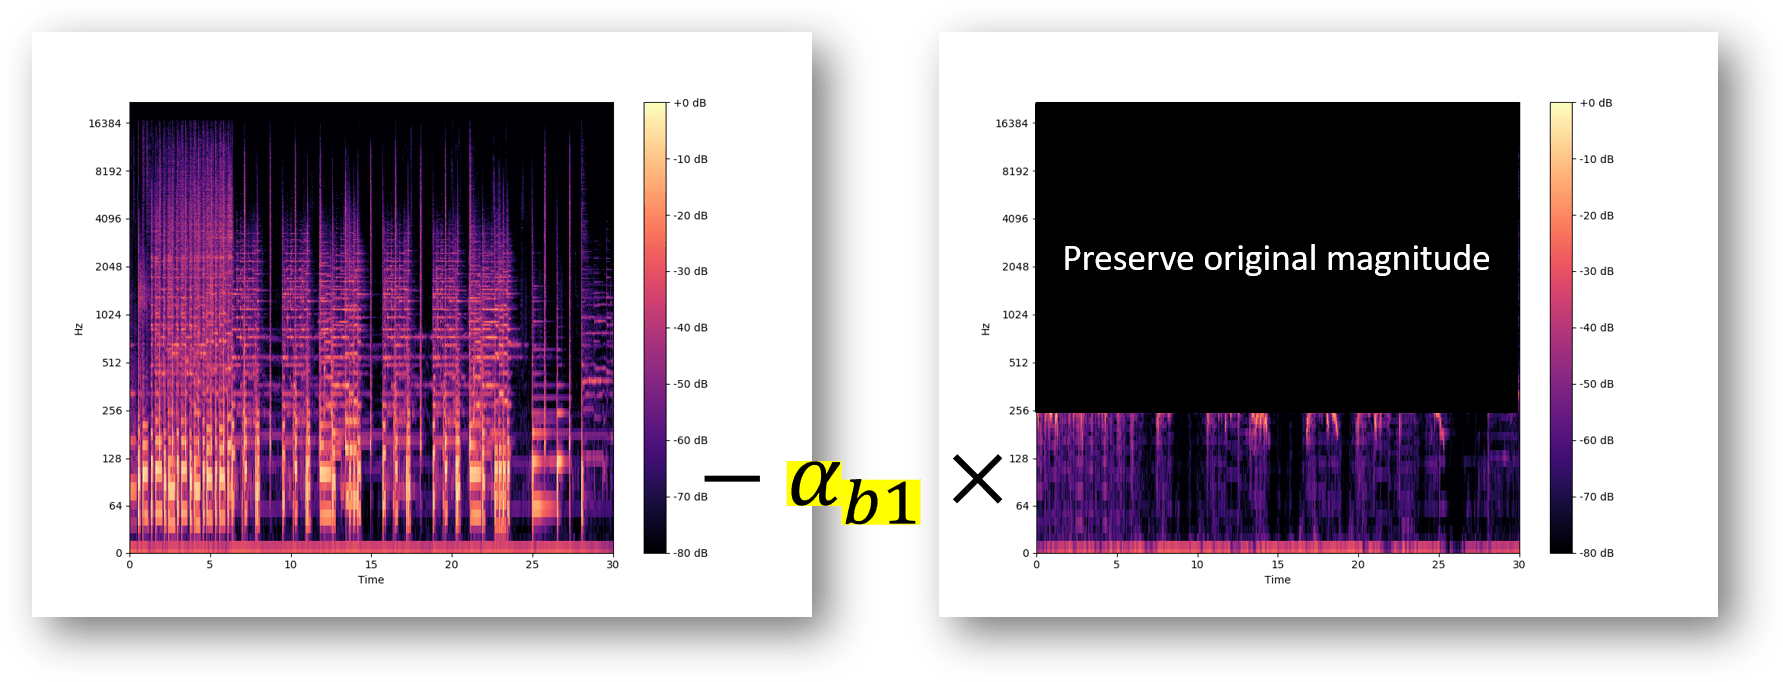
\includegraphics[width=\textwidth]{./figures/chapter04_experiment/Local_Bands_Optimal1.png}
        \caption {Local bands optimal}
        \label{Bands_Optimum_Ratio}
    \end{minipage}
    \hfil
\end{figure}
\begin{figure}[htbp]
    \hfil
    \begin{minipage}[t]{0.65\textwidth}
        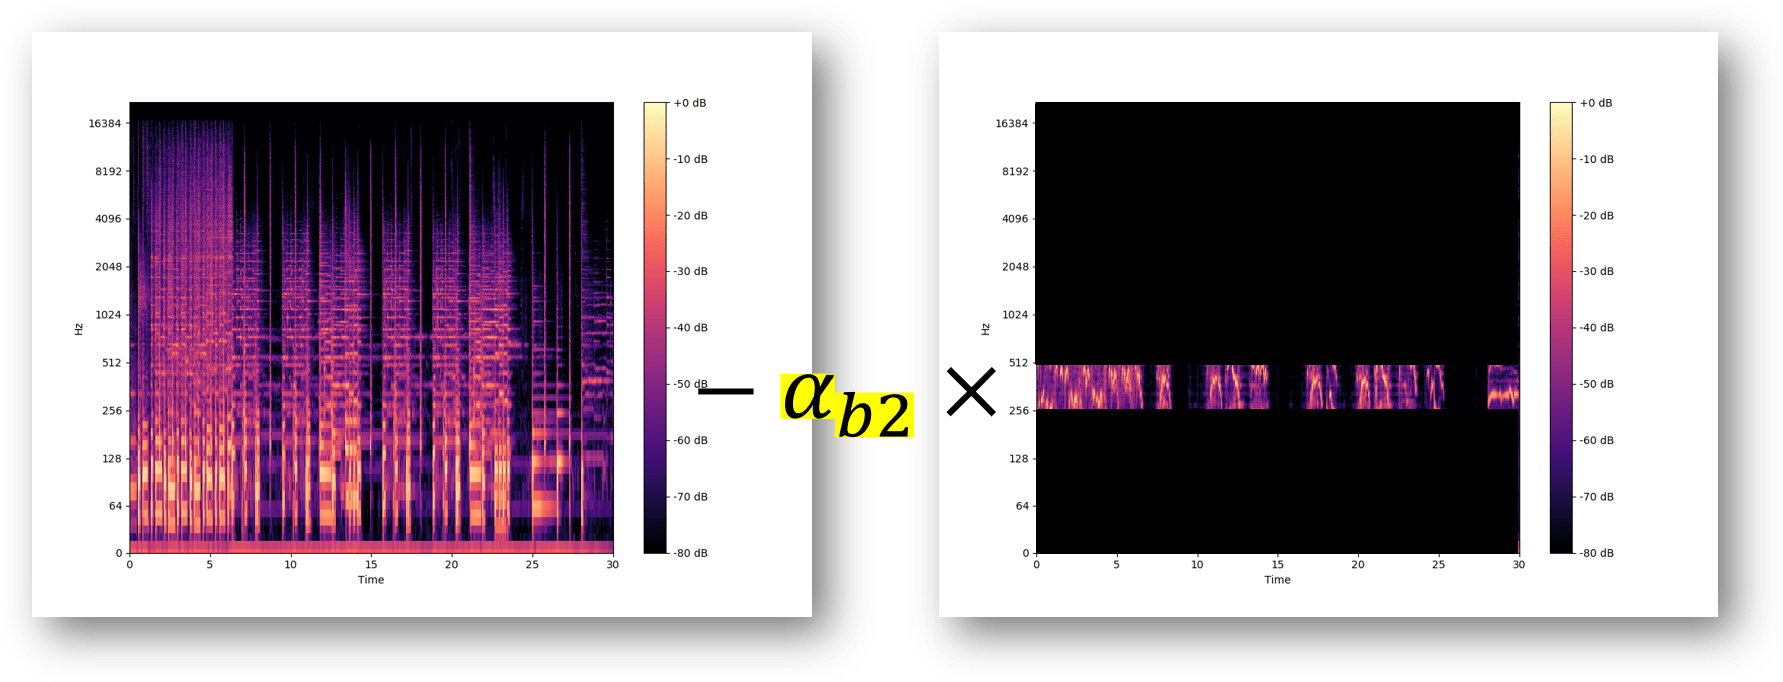
\includegraphics[width=\textwidth]{./figures/chapter04_experiment/Local_Bands_Optimal2.png}
        \caption {Local bands optimal}
        \label{Bands_Optimum_Ratio2}
    \end{minipage}
    \hfil
\end{figure}
\begin{figure}[htbp]
    \hfil
    \begin{minipage}[t]{0.65\textwidth}
        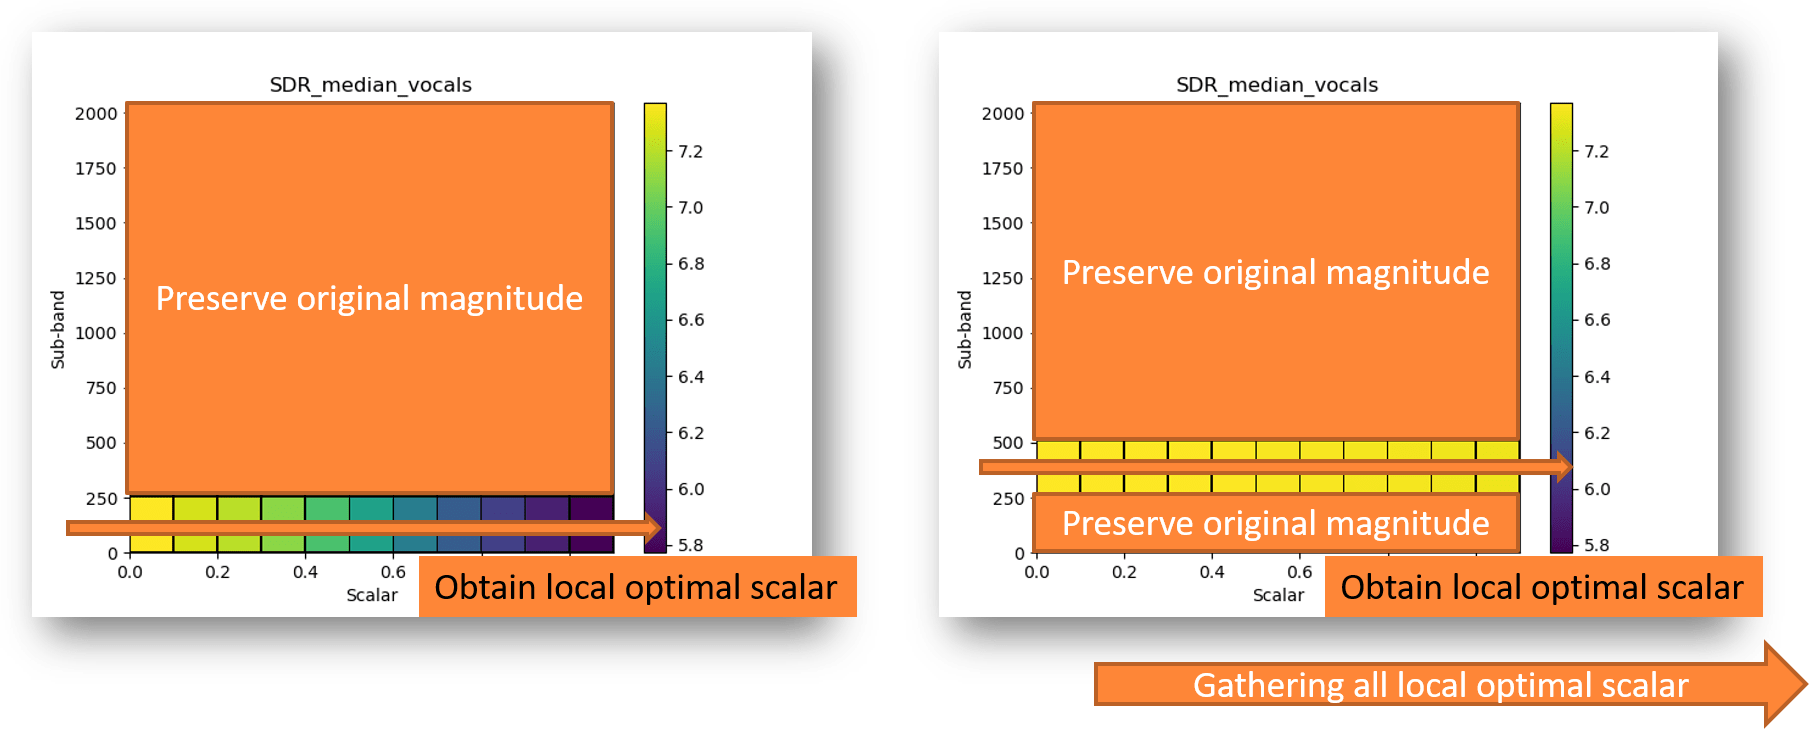
\includegraphics[width=\textwidth]{./figures/chapter04_experiment/Local_Bands_Optimal3.png}
        \caption {Local bands optimal}
        \label{Local_Bands_Optimal3}
    \end{minipage}
    \hfil
\end{figure}

枚舉所有 $\alpha_f$ 難以實現,所以考慮第二種方式,也就是使用簡單的梯度下降架構來訓練,期望每一個 frequency bin (在此研究中總量都為2048個)都能各自算出最好的 $\alpha_f$,改善第一種方式的問題,這邊主要使用最簡單的手法訓練,環繞在一個提出的主架構上(圖\ref{spectrogram_subtraction_NNmethod1}),所有調整架構的實驗中,該架構表現最為出色,其餘架構只以表\ref{spectrogram_subtraction_NNmethod} 呈現,主要討論此方法與第一種方法的差異,而非討論中間梯度下降架構的調整,最終的效果會在下章仔細的探討與分析。梯度下降架構的訓練只在 Musdb18 的訓練集上(共100首),測試集在 Musdb18 的測試集上(共50首),其聲音訊號經由 STFT ,取其 2048 個 frequency bin (F) 與 216 個 frame(T),最後評估的指標使用 Museval。

\begin{table}[htbp]
\centering
\resizebox{\linewidth}{!}{
\begin{tabular}{|c|c|l|l|l|l|l|}
\hline
Magnitude size & 1 layer in neural net & ReLU & Loss function & Batch & Epoch & Optim. method \\ \hline
 & $1\times 2048$ & No & L1Loss & 8 & 200 & ADAM \\ \cline{3-7} 
 & $C\times F$ & No & SmoothL1Loss & 8 & 200 & ADAM \\ \cline{3-7} 
$1\times 2048 \times 512$ & Only apply on stem$_j$ & Yes & L1Loss & 8 & 200 & ADAM \\ \cline{2-7} 
$C\times F\times T$ & $1\times 2048$ & Yes & SmoothL1Loss & 8 & 200 & ADAM \\ \cline{3-7} 
 & $C\times F$ & No & L1Loss & 8 & 200 & ADAM \\ \cline{3-7} 
 & Apply on each stem & No & SmoothL1Loss & 8 & 200 & ADAM \\ \hline
\end{tabular}
}
\caption{過程中梯度下降架構的調整}
\label{spectrogram_subtraction_NNmethod}
\end{table}

\begin{figure}[htbp]
    \hfil
    \begin{minipage}[t]{0.45\textwidth}
        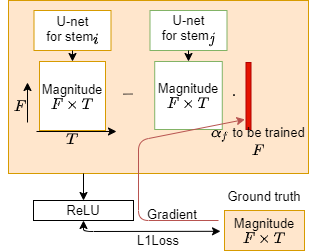
\includegraphics[width=\textwidth]{./figures/chapter04_experiment/spectrogram_subtraction_gradientdecent_method.png}
        \caption {提出的梯度下降架構用以訓練頻譜刪減之對應 $\alpha_f$}
        \label{spectrogram_subtraction_NNmethod1}
    \end{minipage}
    \hfil
\end{figure}

\subsection{注意力模型實驗}
基於 Demucs~\cite{defossez2019music} 與 MMDenseLSTM~\cite{takahashi2018mmdenselstm} 在歌聲分離領域的出眾表現,除了皆以 U-Net 為雛形做衍伸之外,其模型都有個共通點,都使用到了 LSTM~\cite{gers1999learning} 架構,這邊要先稍微提及,此架構起初用在處理長時間序列,可讓深度神經模型觀察到前後文的重複性,透過加入遺忘閥,在遇到長時間輸入訊號時,依舊有不錯的學習效果,但是由於模型結構複雜,因此需要花費較長的時間。歌聲分離領域裡,需要「快」與「準」,除了要準確的預測輸出的音樂訊號,還要夠快,既有的 U-Net 模型預測已經需要不少的時間,如何在觀察前後文的重複性,又要讓模型預測時間不會因此拉長是值得探討的,此時 Google 團隊錄取 2017NIPS\footnote{\url{https://nips.cc/Conferences/2017/Videos}} 的論文「Attention is all you need」~\cite{vaswani2017attention} ,其架構拋棄 RNN 的架構取而代之的是 self-attention 的注意力機制,可以在翻譯領域上有很好的效果,但不導致架構的預測速度。
% file:///C:/Users/hp/Documents/MIR_Lab/report/2Sep2020_report/2Sep2020_report.pdf

% [attention - transformer]
% https://cyeninesky3.medium.com/attention-is-all-you-need-%E5%9F%BA%E6%96%BC%E6%B3%A8%E6%84%8F%E5%8A%9B%E6%A9%9F%E5%88%B6%E7%9A%84%E6%A9%9F%E5%99%A8%E7%BF%BB%E8%AD%AF%E6%A8%A1%E5%9E%8B-dcc12d251449

\subsubsection{Self-attention 架構實驗}
探討在既有的 U-Net 架構~\cite{ronneberger2015u}(圖\ref{Unet_sovia_sattn1}),與 Liu~\cite{liu2020voice} 基於 Dense-UNet~\cite{stoller2018adversarial} 加上 self-attention 架構(圖\ref{Unet_sovia_sattn2})的差異,在下一章可經由實驗結果做比對。
\begin{figure}[htbp]
    \hfil
    \begin{minipage}[t]{0.45\textwidth}
        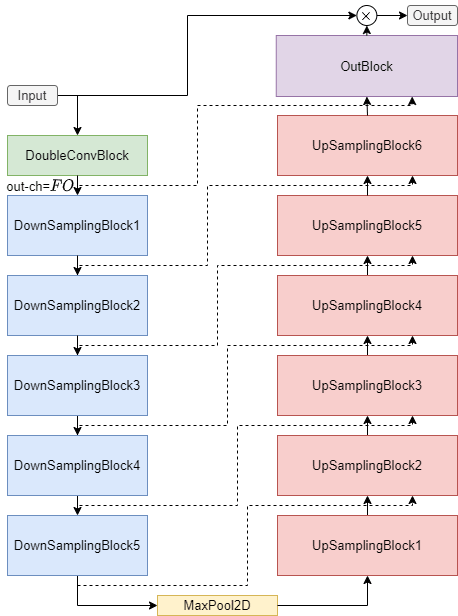
\includegraphics[width=\textwidth]{./figures/chapter04_experiment/Unet_sovia_sattn1.png}
        \caption {既有 U-Net 架構}
        \label{Unet_sovia_sattn1}
    \end{minipage}
    \hfil
\end{figure}
\begin{figure}[htbp]
    \hfil
    \begin{minipage}[t]{0.55\textwidth}
        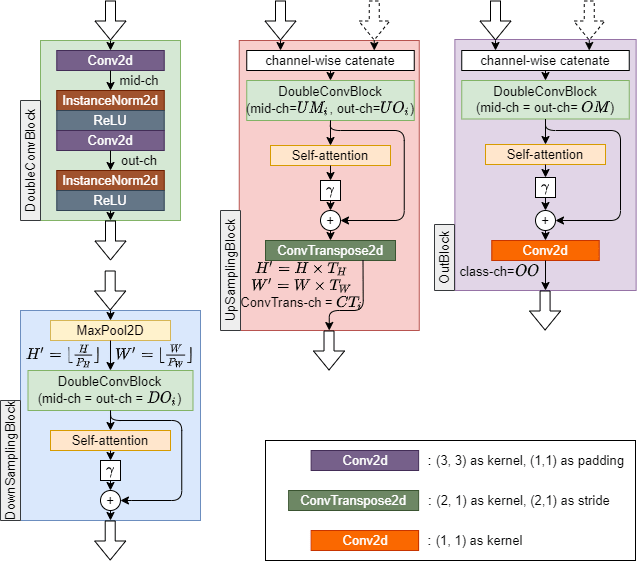
\includegraphics[width=\textwidth]{./figures/chapter04_experiment/Unet_sovia_sattn2.png}
        \caption {對應各子架構}
        \label{Unet_sovia_sattn2}
    \end{minipage}
    \hfil
\end{figure}

適配 self-attention 架構於既有 U-Net 上,做了些許與原文的差異化,本論文將原論文的 $C'$ 設定為 $\left \lfloor C/8 \right \rfloor$而非原文設定的 $C':=5$。另外,U-Net 的 encoder 與 decoder 詳細見下表\ref{UNet_sovia_setting}。

\begin{table}[htbp]
\centering
\begin{tabular}{ccccccc}
\multicolumn{1}{c|}{$i$} & 1 & 2 & 3 & 4 & 5 & 6 \\ \hline
\multicolumn{1}{c|}{$DO_i$} & 32 & 64 & 128 & 256 & 512 &  \\
\multicolumn{1}{c|}{$UM_i$} & 1024 & 512 & 256 & 128 & 64 & 32 \\
\multicolumn{1}{c|}{$UO_i$} & 512 & 256 & 128 & 64 & 32 & 16 \\ \hline
\multicolumn{1}{l}{$FO$=1} & \multicolumn{1}{l}{$OM$=16} & \multicolumn{1}{l}{$OO$=1} & \multicolumn{1}{l}{$P_H$=2} & \multicolumn{1}{l}{$P_W$=1} & \multicolumn{1}{l}{$T_H$=2} & \multicolumn{1}{l}{$T_W$=1}
\end{tabular}
\caption{U-Net6 (baseline) 參數表}
\label{UNet_sovia_setting}
\end{table}

\subsubsection{Attention Gate 架構實驗}
本論文主要探討在既有的 U-Net 架構~\cite{ronneberger2015u}(圖\ref{Unet_sovia_sattn1}),再參考 oktay~\cite{oktay2018attention} 等人提出的 attention U-Net 架構(圖\ref{Unet_sovia_AG1}與圖\ref{Unet_sovia_AG2}),改進既有的 U-Net ,並討論其差異,在下一章可經由實驗結果做比對。可以注意的是圖\ref{attention_gate1} 上的最後有一個調控的 $\alpha$ 參數,為求實驗方便在此固定為 $\alpha:=1$,未來可實驗讓機器自我訓練出該參數的值。

\begin{figure}[htbp]
    \hfil
    \begin{minipage}[t]{0.3\textwidth}
        \centering
        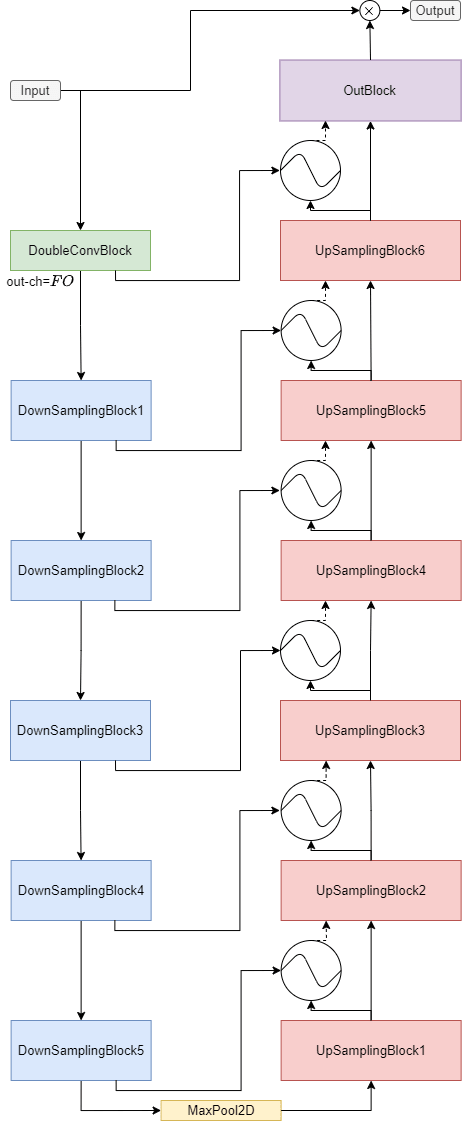
\includegraphics[width=\textwidth]{./figures/chapter04_experiment/Unet_sovia_AG1.png}
        \caption {加上 attention gate 的 U-Net 架構}
        \label{Unet_sovia_AG1}
    \end{minipage}
    \begin{minipage}[t]{0.65\textwidth}
        \centering
        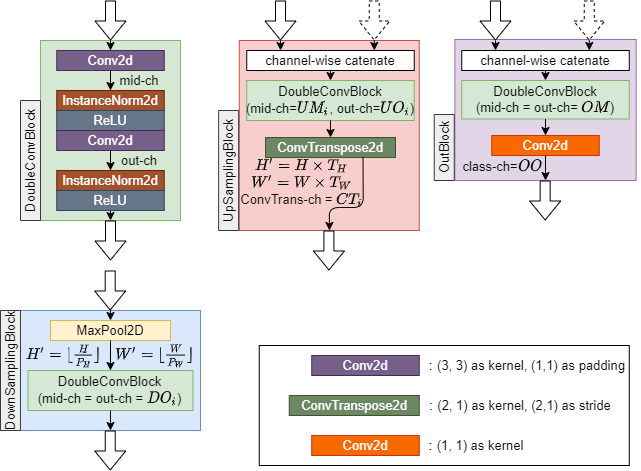
\includegraphics[width=\textwidth]{./figures/chapter04_experiment/Unet_sovia_AG2.png}
        \caption {對應各子架構}
        \label{Unet_sovia_AG2}
    \end{minipage}
    \hfil
\end{figure}

\subsection{模型剪枝實驗}
本論文基於深度可分卷積與 Inverted Residuals 套用在既有 U-Net,前者可以大幅減少模型參數伴隨較大的效能損失,架構細節如圖\ref{MobileUnetV1_1} 與圖\ref{MobileUnetV1_2} ;後者便是稍微對前者方法提升計算量伴隨效果提升,架構細節如圖\ref{MobileUnetV2_1} 與圖\ref{MobileUnetV2_2} 。實際實驗結果在下章討論。

\begin{figure}[htbp]
    \hfil
    \begin{minipage}[t]{0.3\textwidth}
        \centering
        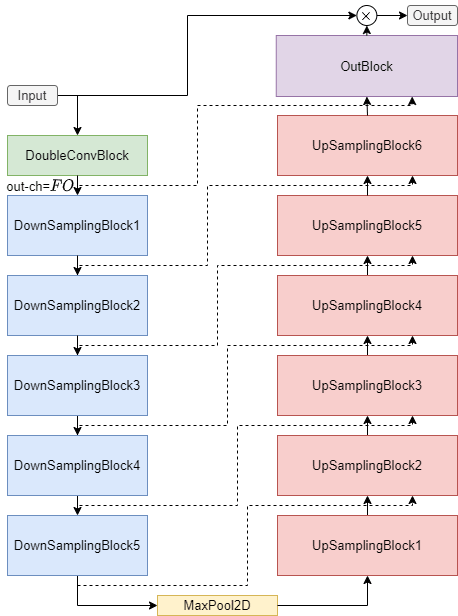
\includegraphics[width=\textwidth]{./figures/chapter04_experiment/MobileUnetV1_1.png}
        \caption {加上深度可分卷積的 U-Net 架構}
        \label{MobileUnetV1_1}
    \end{minipage}
    \begin{minipage}[t]{0.65\textwidth}
        \centering
        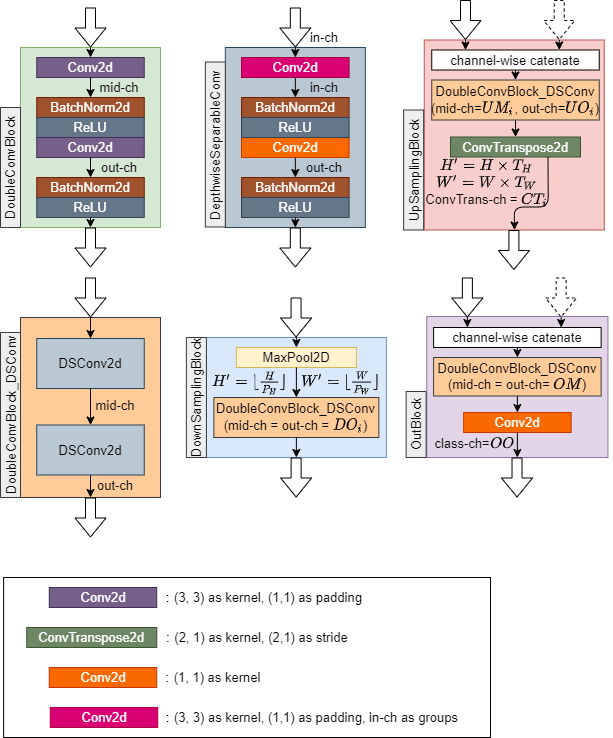
\includegraphics[width=\textwidth]{./figures/chapter04_experiment/MobileUnetV1_2.png}
        \caption {對應各子架構}
        \label{MobileUnetV1_2}
    \end{minipage}
    \hfil
\end{figure}

\begin{figure}[htbp]
    \hfil
    \begin{minipage}[t]{0.3\textwidth}
        \centering
        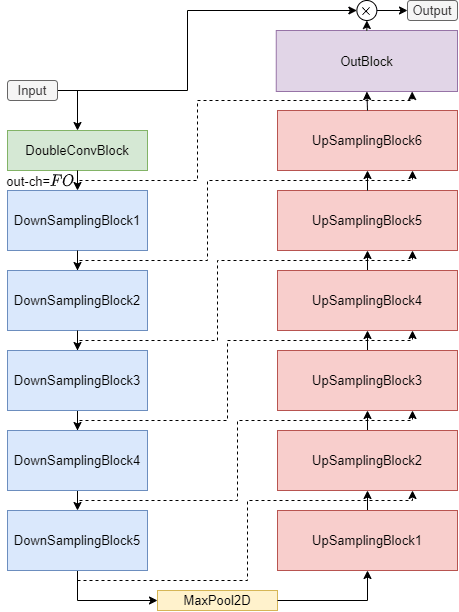
\includegraphics[width=\textwidth]{./figures/chapter04_experiment/MobileUnetV2_1.png}
        \caption {加上 inverted residual block 的 U-Net 架構}
        \label{MobileUnetV2_1}
    \end{minipage}
    \begin{minipage}[t]{0.6\textwidth}
        \centering
        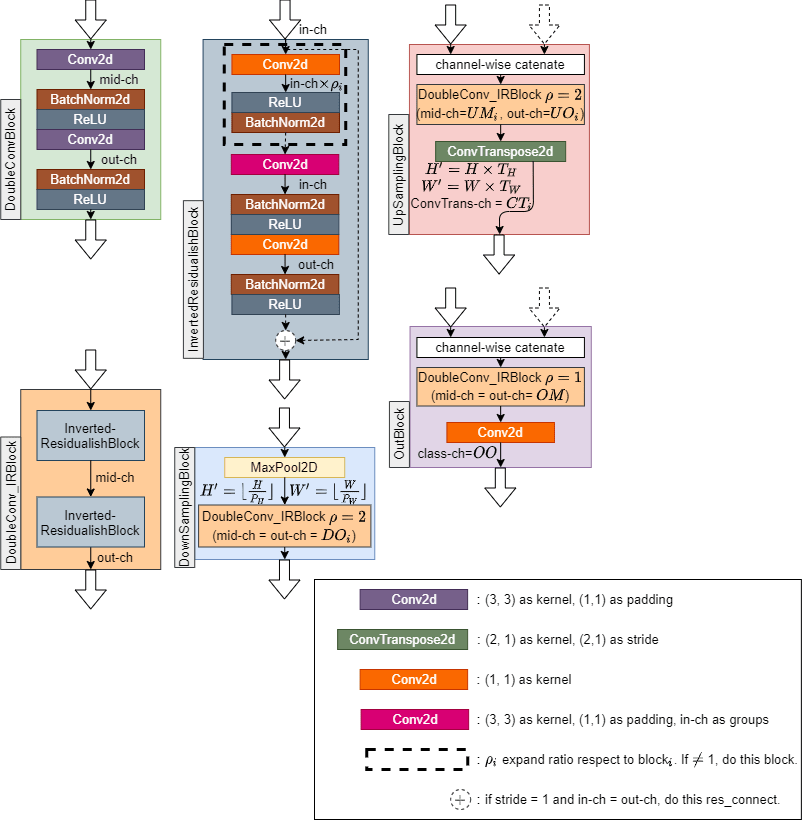
\includegraphics[width=\textwidth]{./figures/chapter04_experiment/MobileUnetV2_2.png}
        \caption {對應各子架構}
        \label{MobileUnetV2_2}
    \end{minipage}
    \hfil
\end{figure}

\clearpage

\subsection{模型量化實驗}
本論文中,主要使用 FaceBook 所提出的 QNNPACK~\cite{dukhan2018qnnpack} 對既有 U-Net 做量化至 int8,值得注意的是,在量化之前,依照常規的手法,會先對模型做融合的操作\footnote{\url{https://pytorch.org/tutorials/recipes/recipes/dynamic_quantization.html}},主要是讓機器在計算 biases 與 ReLU 可以更加快速,其主要的融合方法見圖\ref{quantization2}。

\begin{figure}[htbp]
    \hfil
    \begin{minipage}[t]{1.0\textwidth}
        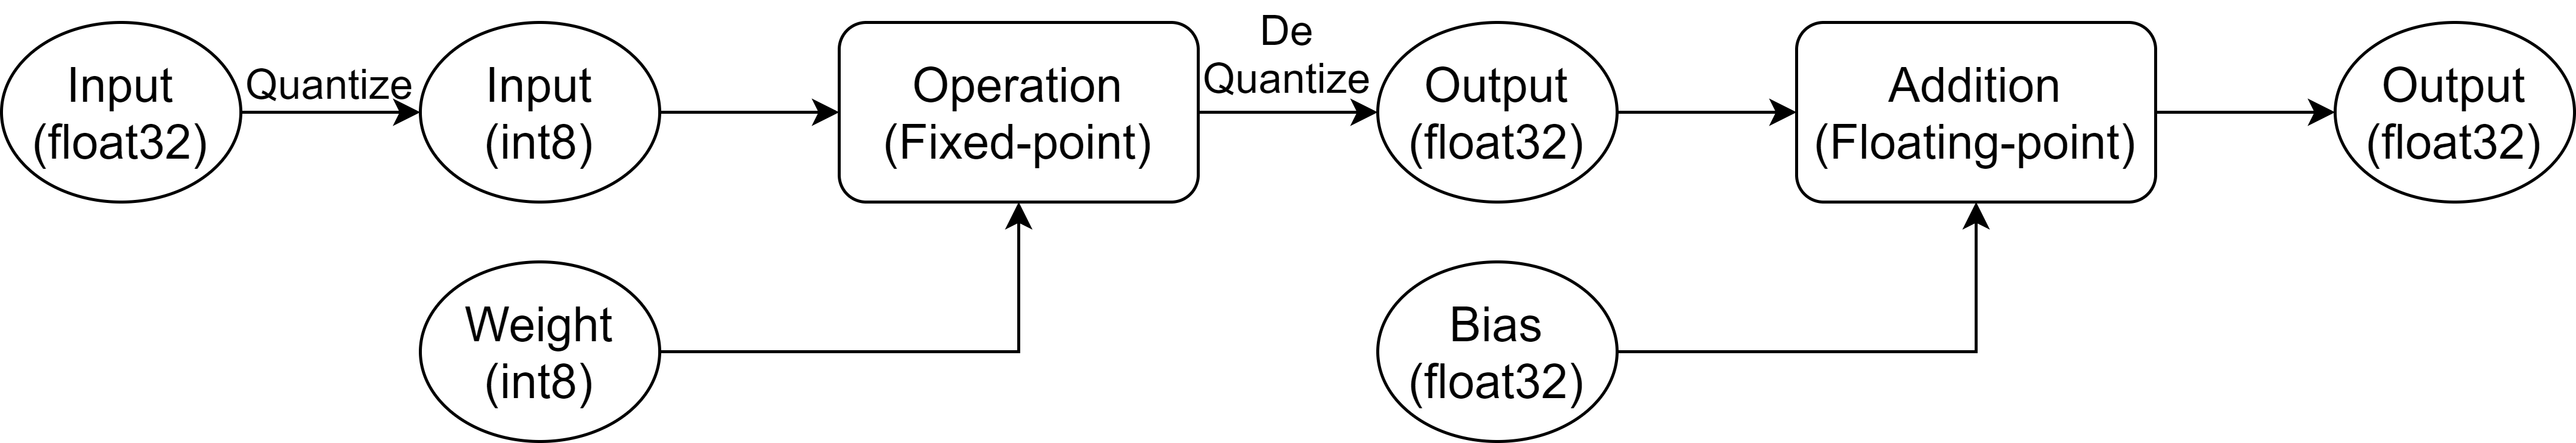
\includegraphics[width=\textwidth]{./figures/chapter04_experiment/quantization2.png}
        \caption {量化過程圖}
        \label{quantization2}
    \end{minipage}
    \hfil
\end{figure}
\chapter{實驗結果討論與錯誤分析}

本章將五個實驗的結果以客觀的指標呈現,並說明實際感受與指標的差異,另外,本研究提出新模型的結果中,本章節提及的結果是只使用到 Musdb18 作為訓練集,這幫助我們可以與其他也只使用該資料集訓練的模型做比較,最後使用額外資料訓練的結果會在附錄中以表格呈現。

\section{實驗一:比較 Ratio Mask 與 Wiener Filter 的效果比較}
U-Net6(baseline)為先前研究提出的架構,且使用所有第三章提及過的資料集訓練。以 U-Net6(baseline)為基準,在後處理的時候做 mulitchannel Wiener filter 與 ratio mask filter,以 museval 檢測(見表\ref{filter_result_table} 與圖\ref{filter_result1} )。在聆聽觀察中,濾波前的伴奏預測軌會有毛邊感(fuzzy sound),為無法完美去除的主唱音軌導致。由圖\ref{filter_result2} 上的主唱軌聲波可明顯看出,濾波可以明顯的提升輸出的效果。mulitchannel Wiener filter 與 ratio mask filter 並無太大差異,但因為實現的細節不同,前者在伴奏軌的效果會比較好,但在聽感上並無太大差異。

\begin{table}[htbp]
\centering
\resizebox{\textwidth}{!}{%
\begin{tabular}{|r|ccc|ccc|}
\hline
 &  & 主唱軌 &  &  & 伴奏軌 &  \\ \hline
 & \multicolumn{1}{c|}{\textbf{SDR}} & \multicolumn{1}{c|}{SIR} & SAR & \multicolumn{1}{c|}{\textbf{SDR}} & \multicolumn{1}{c|}{SIR} & \textbf{SAR} \\ \hline
U-Net6  (baseline) & \multicolumn{1}{c|}{7.269} & \multicolumn{1}{c|}{15.045} & 7.224 & \multicolumn{1}{c|}{13.805} & \multicolumn{1}{c|}{16.785} & 14.520 \\ \hline
U-Net6  (baseline) w/ MWF & \multicolumn{1}{c|}{\textbf{7.648}} & \multicolumn{1}{c|}{18.593} & 7.436 & \multicolumn{1}{c|}{\textbf{14.288}} & \multicolumn{1}{c|}{20.332} & \textbf{14.815} \\ \hline
U-Net6  (baseline) w/ ratio mask filter & \multicolumn{1}{c|}{\textbf{7.648}} & \multicolumn{1}{c|}{18.585} & 7.435 & \multicolumn{1}{c|}{14.194} & \multicolumn{1}{c|}{20.221} & 14.758 \\ \hline
\end{tabular}%
}
\caption{實驗數據表}
\label{filter_result_table}
\end{table}

\begin{figure}[htbp]
    \hfil
    \begin{minipage}[t]{1.0\textwidth}
        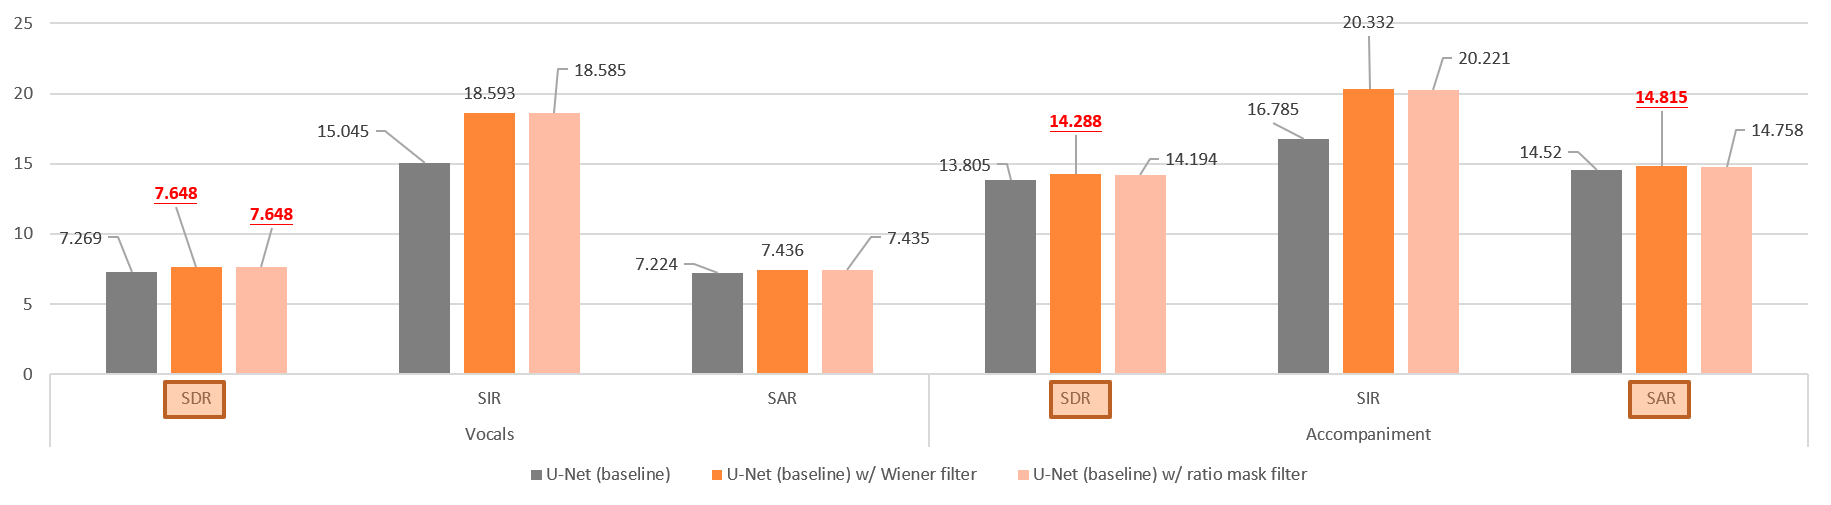
\includegraphics[width=\textwidth]{./figures/chapter05_result/filter_result1.png}
        \caption {濾波實驗長條圖}
        \label{filter_result1}
    \end{minipage}
    \hfil
\end{figure}

\begin{figure}[htbp]
    \hfil
    \begin{minipage}[t]{1.0\textwidth}
        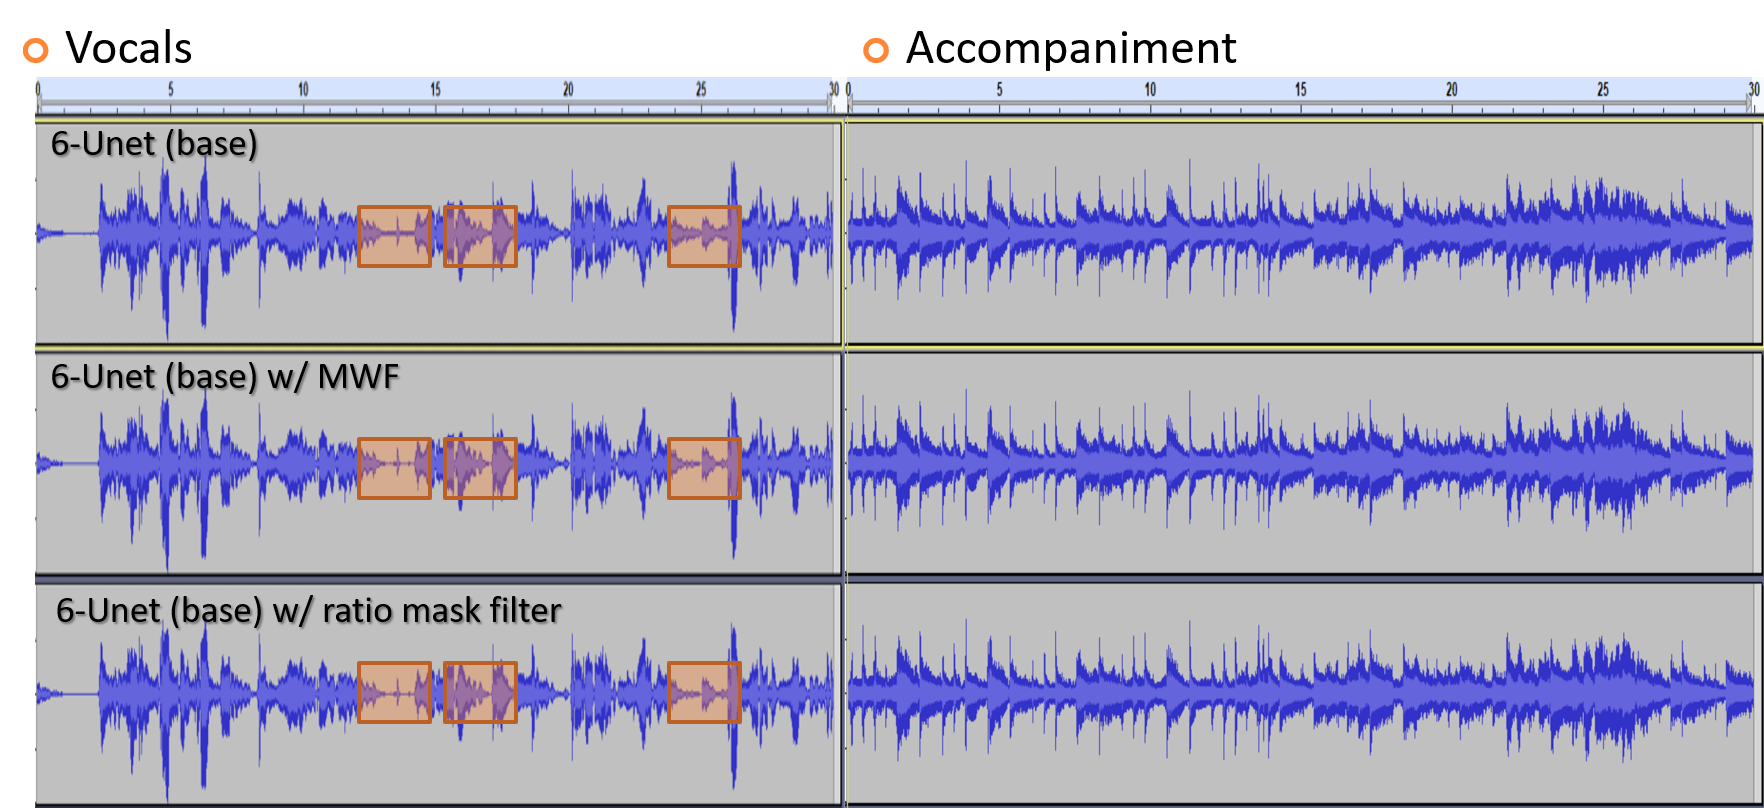
\includegraphics[width=\textwidth]{./figures/chapter05_result/filter_result2.png}
        \caption {濾波實驗效果圖}
        \label{filter_result2}
    \end{minipage}
    \hfil
\end{figure}

\clearpage

\section{實驗二:頻譜刪減法效果比較}
% 補 nn 方法的 alpha_f 圖
此實驗是基於先前實驗的效果,在 $\alpha=0.2$ 的時候,其效果有些許地增幅,但這是對於每個 frequency bin 都使用同一個頻譜刪減幅度,本輪文提出兩個方法希望可對每個 $f \in F$ 各自求取最好的刪減幅度 $\alpha$,其效果以 museval 做檢測(見表\ref{magnitude_subtraction_method_table} 與圖\ref{magnitude_subtraction_method_result1})。

\begin{table}[htbp]
\centering
\resizebox{\textwidth}{!}{%
\begin{tabular}{|r|ccc|ccc|c|}
\hline
 &  & 主唱軌 &  &  & 伴奏軌 &  & Note \\ \hline
 & \multicolumn{1}{c|}{\textbf{SDR}} & \multicolumn{1}{c|}{SIR} & SAR & \multicolumn{1}{c|}{\textbf{SDR}} & \multicolumn{1}{c|}{SIR} & \textbf{SAR} &  \\ \hline
\textit{U-Net6 (baseline)} & \multicolumn{1}{c|}{\textit{7.269}} & \multicolumn{1}{c|}{\textit{15.045}} & \textit{7.224} & \multicolumn{1}{c|}{\textit{13.085}} & \multicolumn{1}{c|}{\textit{16.785}} & \textit{14.751} &  \\ \hline
0.2 as ratio for each bins & \multicolumn{1}{c|}{\textbf{7.352}} & \multicolumn{1}{c|}{18.748} & 7.146 & \multicolumn{1}{c|}{\textbf{14.031}} & \multicolumn{1}{c|}{20.728} & 14.151 & 先前實驗 \\ \hline
Band-based optimal ratio & \multicolumn{1}{c|}{7.346} & \multicolumn{1}{c|}{16.077} & 7.507 & \multicolumn{1}{c|}{13.988} & \multicolumn{1}{c|}{19.185} & 14.147 & 本次實驗 \\ \hline
Frequency-based optimal ratio & \multicolumn{1}{c|}{7.340} & \multicolumn{1}{c|}{15.704} & 7.345 & \multicolumn{1}{c|}{13.895} & \multicolumn{1}{c|}{17.151} & \textbf{14.634} & 本次實驗 \\ \hline
\end{tabular}%
}
\caption{頻譜刪減幅度實驗比較表}
\label{magnitude_subtraction_method_table}
\end{table}

\begin{figure}[htbp]
    \hfil
    \begin{minipage}[t]{1.0\textwidth}
        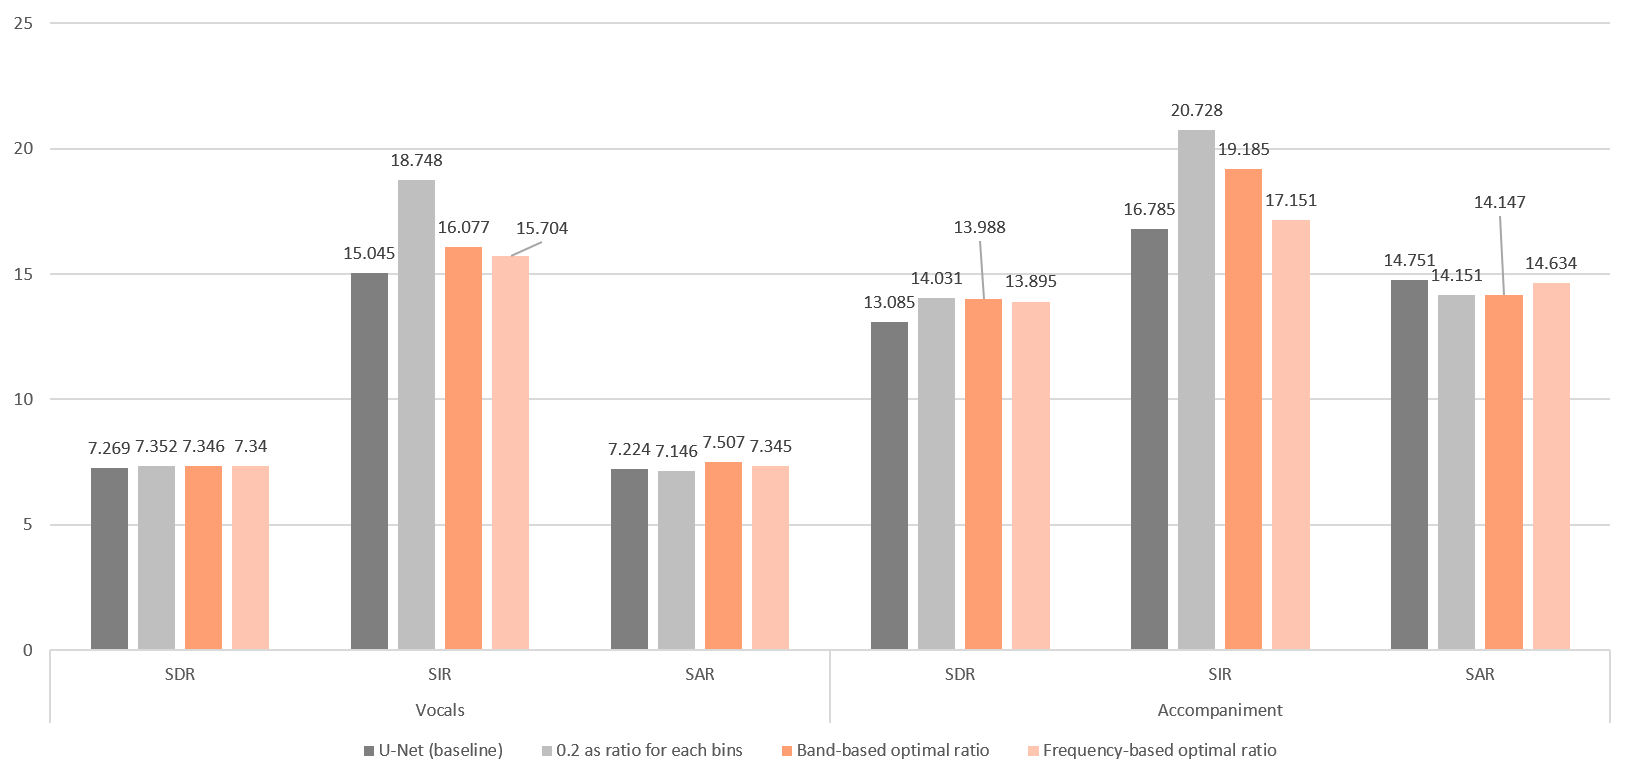
\includegraphics[width=\textwidth]{./figures/chapter05_result/magnitude_subtraction_method_result1.png}
        \caption {頻譜刪減幅度實驗比較表}
        \label{magnitude_subtraction_method_result1}
    \end{minipage}
    \hfil
\end{figure}

第一個方法對於每個頻帶 $b\in Bands$ 求取頻譜刪減幅度 $\alpha_b$,圖\ref{magnitude_subtraction_method_result2} 表示出對應的刪減幅度值,左為主唱軌的刪減幅度,右為伴奏軌的刪減幅度。

\begin{figure}[htbp]
    \hfil
    \begin{minipage}[t]{0.6\textwidth}
        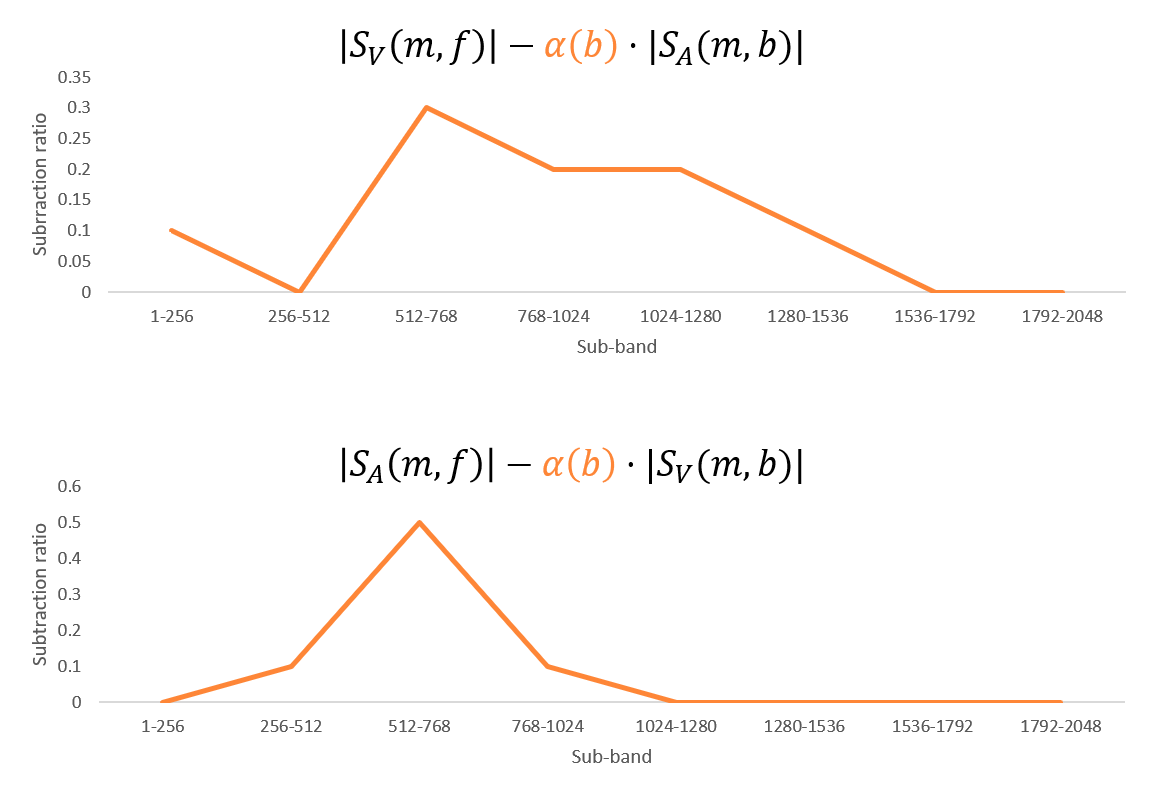
\includegraphics[width=\textwidth]{./figures/chapter05_result/magnitude_subtraction_method_result2.png}
        \caption {實驗方法一取得的各個 $\alpha_b$}
        \label{magnitude_subtraction_method_result2}
    \end{minipage}
    \hfil
\end{figure}

第二個方法對於每個 $f\in F$ 求取頻譜刪減幅度 $\alpha_f$,圖\ref{magnitude_subtraction_method2_result1} 與圖\ref{magnitude_subtraction_method2_result2}  表示出對應的刪減幅度值,圖\ref{magnitude_subtraction_method2_result1} 為主唱軌被刪減時乘上的幅度,圖\ref{magnitude_subtraction_method2_result2} 為伴奏軌被刪減時乘上的幅度。

\begin{figure}[htbp]
    \hfil
    \begin{minipage}[t]{0.6\textwidth}
        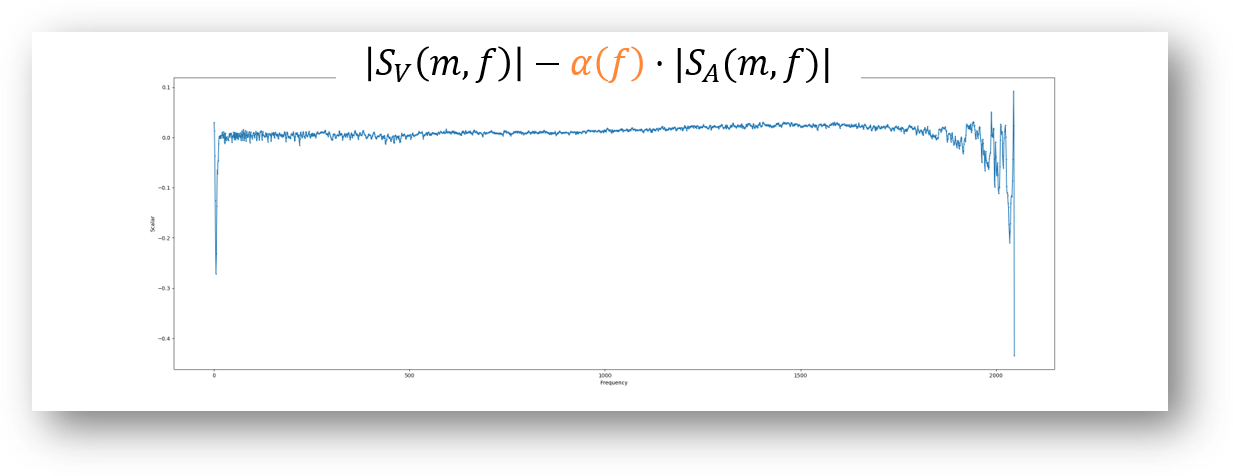
\includegraphics[width=\textwidth]{./figures/chapter05_result/spectrogram_subtraction_nn_accompaniment-vocals_T-216.png}
        \caption {實驗方法二取得的各個 $\alpha_f$}
        \label{magnitude_subtraction_method2_result1}
    \end{minipage}
    \hfil
\end{figure}
\begin{figure}[htbp]
    \hfil
    \begin{minipage}[t]{0.6\textwidth}
        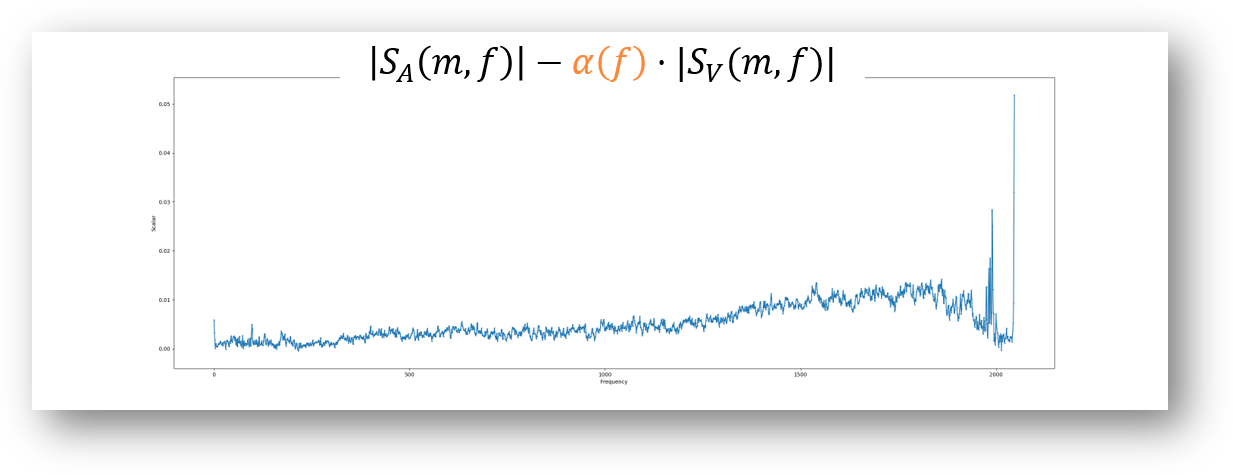
\includegraphics[width=\textwidth]{./figures/chapter05_result/spectrogram_subtraction_nn_vocals-accompaniment_T-216.png}
        \caption {實驗方法二取得的各個 $\alpha_f$}
        \label{magnitude_subtraction_method2_result2}
    \end{minipage}
    \hfil
\end{figure}

在 frequency-based optimal ratio 實驗中, initial weight 對於梯度下降法也會有所影響,上面的結果是對 initial weight 設定為 0。在這邊作者另外嘗試對 initial weight 設定為 0.2 時的效果,可以觀察到,取得的 $\alpha_f$ (圖\ref{magnitude_subtraction_method2_result3}、圖\ref{magnitude_subtraction_method2_result4} )會有變化,但在效果來說,並沒有差異太大 (表\ref{frequency-based_init_weight_table}、圖\ref{magnitude_subtraction_method_result3})。

\begin{figure}[htbp]
    \hfil
    \begin{minipage}[t]{0.6\textwidth}
        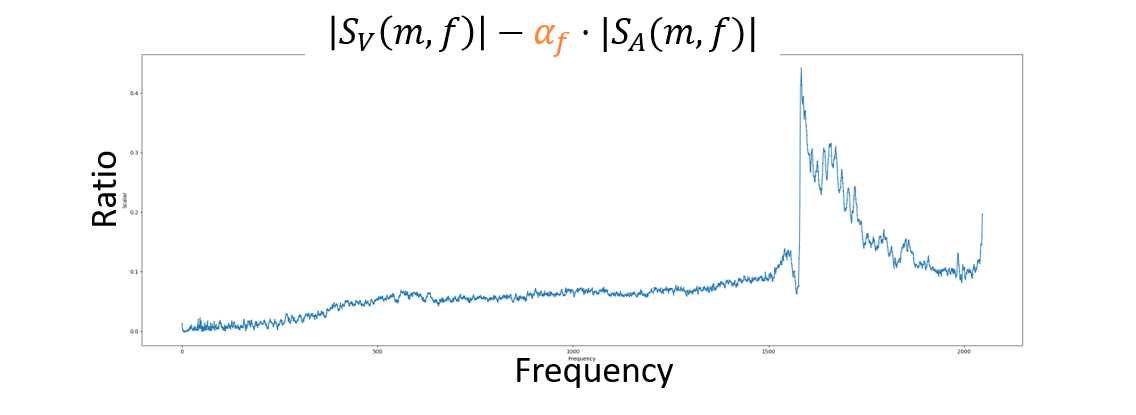
\includegraphics[width=\textwidth]{./figures/chapter05_result/init0.2_spectrogram_subtraction_nn_accompaniment-vocals_T-216.png}
        \caption {Initial weight 設為 0.2 時,frequency-based optimal ratio 取得到的 $\alpha_f$}
        \label{magnitude_subtraction_method2_result3}
    \end{minipage}
    \hfil
\end{figure}
\begin{figure}[htbp]
    \hfil
    \begin{minipage}[t]{0.6\textwidth}
        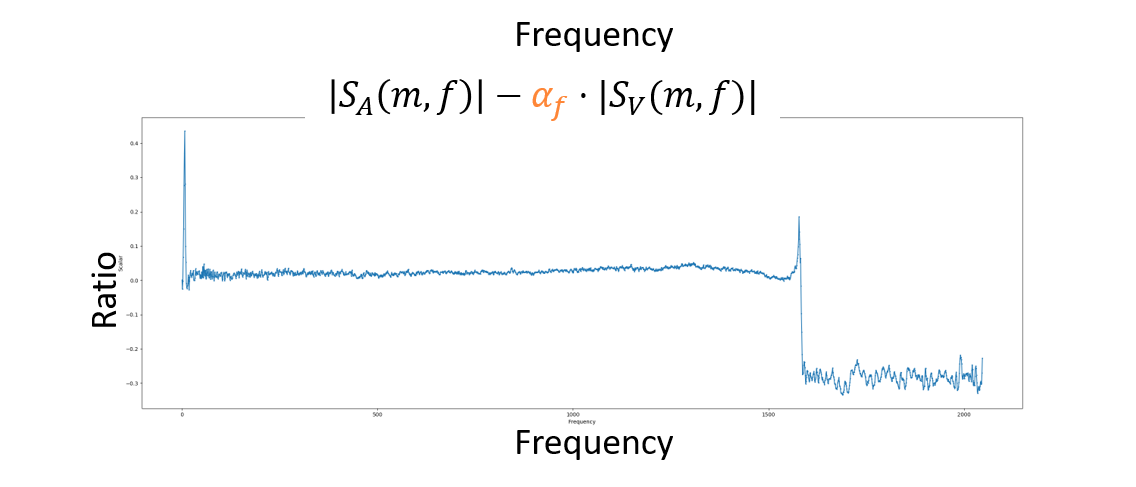
\includegraphics[width=\textwidth]{./figures/chapter05_result/init0.2_spectrogram_subtraction_nn_vocals-accompaniment_T-216.png}
        \caption {Initial weight 設為 0.2 時,frequency-based optimal ratio 取得到的 $\alpha_f$}
        \label{magnitude_subtraction_method2_result4}
    \end{minipage}
    \hfil
\end{figure}

\begin{table}[htbp]
\centering
\begin{tabular}{|r|c|c|c|c|c|c|}
\hline
\multicolumn{1}{|l|}{} & \multicolumn{3}{c|}{主唱軌} & \multicolumn{3}{c|}{伴奏軌} \\ \hline
\multicolumn{1}{|l|}{} & SDR & SIR & SAR & SDR & SIR & SAR \\ \hline
U-Net6 (baseline) & 7.269 & 15.045 & 7.224 & 13.085 & 16.785 & 14.751 \\ \hline
0.2 as ratio for each bins & 7.352 & 18.748 & 7.146 & 14.031 & 20.728 & 14.151 \\ \hline
w/ initial weight 0 & 7.34 & 15.704 & 7.345 & 13.895 & 17.151 & 14.634 \\ \hline
w/ initial weight 0.2 & 7.345 & 15.839 & 7.347 & 13.894 & 17.24 & 14.62 \\ \hline
\end{tabular}
\caption{Initial weight 設為 0.2 後的差異}
\label{frequency-based_init_weight_table}
\end{table}

\begin{figure}[htbp]
    \hfil
    \begin{minipage}[t]{1.0\textwidth}
        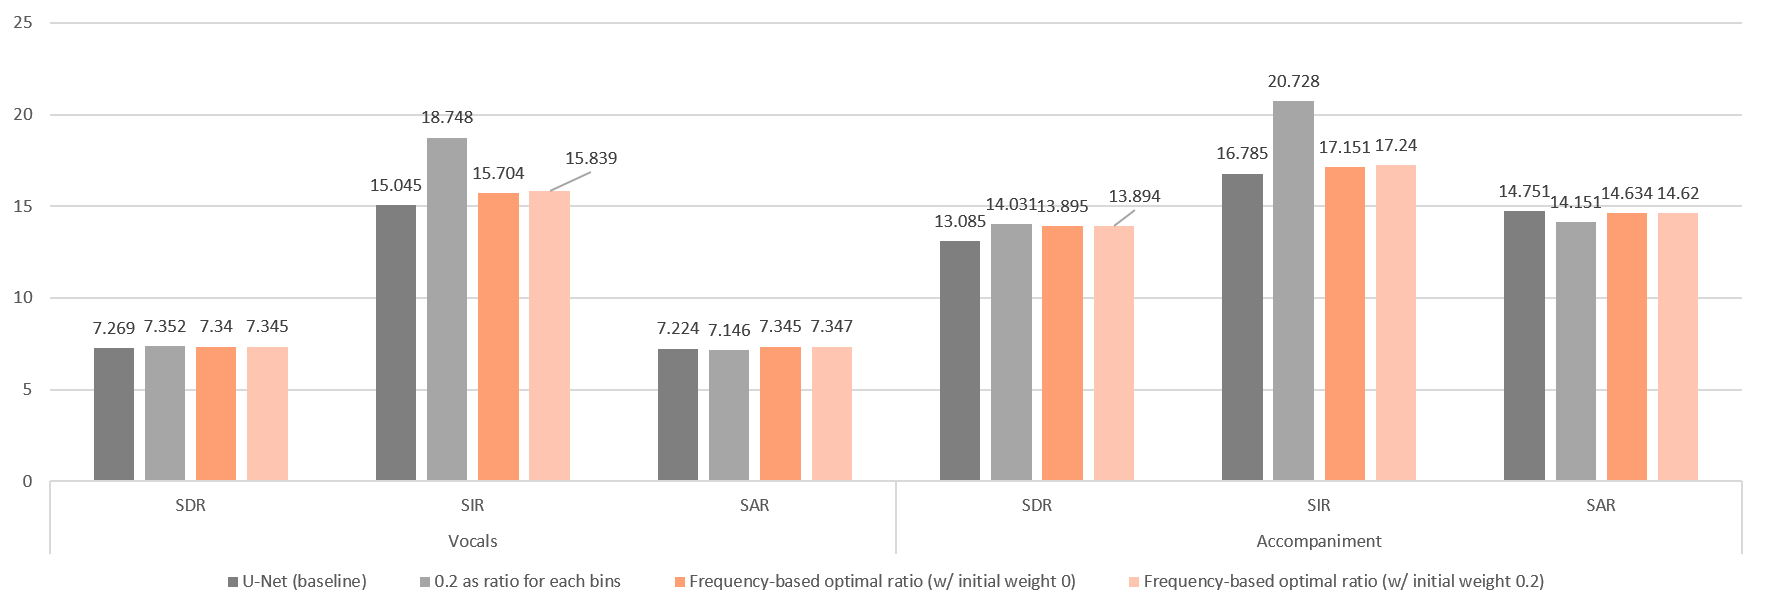
\includegraphics[width=\textwidth]{./figures/chapter05_result/magnitude_subtraction_method_result3.png}
        \caption {Initial weight 設為 0.2 後的差異}
        \label{magnitude_subtraction_method_result3}
    \end{minipage}
    \hfil
\end{figure}

\subsection*{錯誤分析}
與先前實驗的效果比較起來,本論文提出的方法雖有提升輸出音訊的效果,但無法勝過先前是必續探討的,本段落會提些見解,並在未來逐一克服。

關於第一個方法取得每個頻帶的刪減幅度 $\alpha_b$ ,其方法可能太過簡化,無法枚舉所有可能的排列組合,因為在找尋其中一個頻帶 $b_i$ 時,其餘的頻帶是不去考慮其刪減幅度,這可能也帶表了兩件事:區域的最佳解不能代表全域的解、區域枚舉的 $\alpha_{b_i}$ 粒度可能不夠細。可能使用 fmin search 的方式解此問題,直接定義其數學式找到最佳解,但這必須在未來慢慢探討。

關於第二個方法取得每個頻率的刪減幅度 $\alpha_f$,其問題也分成幾層面。第一個問題,可能架構不適合此問題,需要再確認該輸入資訊的特性,以修改訓練的模型。第二個問題,是否只需第一種解決方案即可。

\clearpage

\section{實驗三:不同注意力模型效果比較}
修改原始模型中,U-Net6(baseline)程式維護度差與延展性差(No scalability )難以更改,因此先重新設計,轉換到另一個可維護且延展性好的 U-Net6\_s(convtranspose)。U-Net6 (AG) 與 U-Net6 (Sattn) 皆使用 U-Net6\_s(convtranspose)為基礎來開發(表\ref{attention_based_unet_table1}),架構在第四章以圖解釋。其中 U-Net6 (Sattn) 在伴奏預測效果最好(見表\ref{attention_based_unet_table2} 與圖\ref{attention_based_unet_result1}),但也是模型最龐大的,可以證明 self-attention 有助於時間軸上找到相同特徵序,聽感上,原本主唱預測軌難以去除的鼓聲也可以有效的解決(也可從圖\ref{U-Net6(baseline)_vocals} 與圖\ref{U-Net6(Sattn)_vocals} 上觀察頻譜中鼓在高頻能量已經消失,被 self-attention 的 U-Net 解決)。

\begin{figure}[htbp]
    \hfil
    \begin{minipage}[t]{0.45\textwidth}
        \centering
        % time series body
        \begin{tikzpicture}[scale=0.75]
        \begin{semilogyaxis} [
            xlabel = Epoch,
            ylabel = Loss,
        ]
            \addlegendentry{Training loss}
            \addplot table[mark=none, x=Step,y=Value, col sep=comma] {./numerical-data/chapter05_result/experiment03/6-Unet (base)/accompaniment/trnloss.csv};
            \addlegendentry{Validation loss}
            \addplot table[mark=none, x=Step,y=Value, col sep=comma] {./numerical-data/chapter05_result/experiment03/6-Unet (base)/accompaniment/valloss.csv};
        \end{semilogyaxis}
        \end{tikzpicture}
        % time series body
        \caption {U-Net6 (baseline) 對伴奏軌訓練的 loss}
        \label{e3:6-Unet (base):accompaniment}
    \end{minipage}
    \begin{minipage}[t]{0.45\textwidth}
        \centering
        % time series body
        \begin{tikzpicture}[scale=0.75]
        \begin{semilogyaxis} [
            xlabel = Epoch,
            ylabel = Loss,
        ]
            \addlegendentry{Training loss}
            \addplot table[mark=none, x=Step,y=Value, col sep=comma] {./numerical-data/chapter05_result/experiment03/6-Unet (base)/vocals/trnloss.csv};
            \addlegendentry{Validation loss}
            \addplot table[mark=none, x=Step,y=Value, col sep=comma] {./numerical-data/chapter05_result/experiment03/6-Unet (base)/vocals/valloss.csv};
        \end{semilogyaxis}
        \end{tikzpicture}
        % time series body
        \caption {U-Net6 (baseline) 對主唱軌訓練的 loss}
        \label{e3:6-Unet (base):vocals}
    \end{minipage}
    \hfil
\end{figure}


\begin{figure}[htbp]
    \hfil
    \begin{minipage}[t]{0.45\textwidth}
        \centering
        % time series body
        \begin{tikzpicture}[scale=0.75]
        \begin{semilogyaxis} [
            xlabel = Epoch,
            ylabel = Loss,
        ]
            \addlegendentry{Training loss}
            \addplot table[mark=none, x=Step,y=Value, col sep=comma] {./numerical-data/chapter05_result/experiment03/V1 6-Unet (convtranspose)/accompaniment/trnloss.csv};
            \addlegendentry{Validation loss}
            \addplot table[mark=none, x=Step,y=Value, col sep=comma] {./numerical-data/chapter05_result/experiment03/V1 6-Unet (convtranspose)/accompaniment/valloss.csv};
        \end{semilogyaxis}
        \end{tikzpicture}
        % time series body
        \caption {U-Net6\_s (convtranspose) 對伴奏軌訓練的 loss}
        \label{e3:V1 6-Unet (convtranspose):accompaniment}
    \end{minipage}
    \begin{minipage}[t]{0.45\textwidth}
        \centering
        % time series body
        \begin{tikzpicture}[scale=0.75]
        \begin{semilogyaxis} [
            xlabel = Epoch,
            ylabel = Loss,
        ]
            \addlegendentry{Training loss}
            \addplot table[mark=none, x=Step,y=Value, col sep=comma] {./numerical-data/chapter05_result/experiment03/V1 6-Unet (convtranspose)/vocals/trnloss.csv};
            \addlegendentry{Validation loss}
            \addplot table[mark=none, x=Step,y=Value, col sep=comma] {./numerical-data/chapter05_result/experiment03/V1 6-Unet (convtranspose)/vocals/valloss.csv};
        \end{semilogyaxis}
        \end{tikzpicture}
        % time series body
        \caption {U-Net6\_s (convtranspose) 對主唱軌訓練的 loss}
        \label{e3:V1 6-Unet (convtranspose):vocals}
    \end{minipage}
    \hfil
\end{figure}

\begin{figure}[htbp]
    \hfil
    \begin{minipage}[t]{0.45\textwidth}
        \centering
        % time series body
        \begin{tikzpicture}[scale=0.75]
        \begin{semilogyaxis} [
            xlabel = Epoch,
            ylabel = Loss,
        ]
            \addlegendentry{Training loss}
            \addplot table[mark=none, x=Step,y=Value, col sep=comma] {./numerical-data/chapter05_result/experiment03/6-Unet (AG_C-V1)/accompaniment/trnloss.csv};
            \addlegendentry{Validation loss}
            \addplot table[mark=none, x=Step,y=Value, col sep=comma] {./numerical-data/chapter05_result/experiment03/6-Unet (AG_C-V1)/accompaniment/valloss.csv};
        \end{semilogyaxis}
        \end{tikzpicture}
        % time series body
        \caption {U-Net6 (AG) 對伴奏軌訓練的 loss}
        \label{e3:6-Unet (AG_C-V1):accompaniment}
    \end{minipage}
    \begin{minipage}[t]{0.45\textwidth}
        \centering
        % time series body
        \begin{tikzpicture}[scale=0.75]
        \begin{semilogyaxis} [
            xlabel = Epoch,
            ylabel = Loss,
        ]
            \addlegendentry{Training loss}
            \addplot table[mark=none, x=Step,y=Value, col sep=comma] {./numerical-data/chapter05_result/experiment03/6-Unet (AG_C-V1)/vocals/trnloss.csv};
            \addlegendentry{Validation loss}
            \addplot table[mark=none, x=Step,y=Value, col sep=comma] {./numerical-data/chapter05_result/experiment03/6-Unet (AG_C-V1)/vocals/valloss.csv};
        \end{semilogyaxis}
        \end{tikzpicture}
        % time series body
        \caption {U-Net6 (AG) 對主唱軌訓練的 loss}
        \label{e3:6-Unet (AG_C-V1):vocals}
    \end{minipage}
    \hfil
\end{figure}

\begin{figure}[htbp]
    \hfil
    \begin{minipage}[t]{0.45\textwidth}
        \centering
        % time series body
        \begin{tikzpicture}[scale=0.75]
        \begin{semilogyaxis} [
            xlabel = Epoch,
            ylabel = Loss,
        ]
            \addlegendentry{Training loss}
            \addplot table[mark=none, x=Step,y=Value, col sep=comma] {./numerical-data/chapter05_result/experiment03/6-Unet (Sattn_C-V4)/accompaniment/trnloss.csv};
            \addlegendentry{Validation loss}
            \addplot table[mark=none, x=Step,y=Value, col sep=comma] {./numerical-data/chapter05_result/experiment03/6-Unet (Sattn_C-V4)/accompaniment/valloss.csv};
        \end{semilogyaxis}
        \end{tikzpicture}
        % time series body
        \caption {U-Net6 (Sattn) 對伴奏軌訓練的 loss}
        \label{e3:6-Unet (Sattn_C-V4):accompaniment}
    \end{minipage}
    \begin{minipage}[t]{0.45\textwidth}
        \centering
        % time series body
        \begin{tikzpicture}[scale=0.75]
        \begin{semilogyaxis} [
            xlabel = Epoch,
            ylabel = Loss,
        ]
            \addlegendentry{Training loss}
            \addplot table[mark=none, x=Step,y=Value, col sep=comma] {./numerical-data/chapter05_result/experiment03/6-Unet (Sattn_C-V4)/vocals/trnloss.csv};
            \addlegendentry{Validation loss}
            \addplot table[mark=none, x=Step,y=Value, col sep=comma] {./numerical-data/chapter05_result/experiment03/6-Unet (Sattn_C-V4)/vocals/valloss.csv};
        \end{semilogyaxis}
        \end{tikzpicture}
        % time series body
        \caption {U-Net6 (Sattn) 對主唱軌訓練的 loss}
        \label{e3:6-Unet (Sattn_C-V4):vocals}
    \end{minipage}
    \hfil
\end{figure}

\begin{table}[htbp]
\centering
\resizebox{\textwidth}{!}{%
\begin{tabular}{|r|c|c|l|}
\hline
 & Size (MB) & Normalization method & Note \\ \hline
U-Net6 (baseline) & 118.9 &  & No scalability \\ \cline{1-2}
U-Net6\_s (convtranspose) & 118.84 & Instance normalization & Scalability \\ \cline{1-2}
U-Net6 (AG) & 120.3 &  & Attention gate \\ \cline{1-2}
U-Net6 (Sattn) & 135.49 &  & Self-attention \\ \hline
\end{tabular}%
}
\caption{注意力 U-Net 架構的比較}
\label{attention_based_unet_table1}
\end{table}

\begin{table}[htbp]
\centering
\resizebox{\textwidth}{!}{%
\begin{tabular}{|r|ccc|ccc|}
\hline
 &  & 主唱軌 &  &  & 伴奏軌 &  \\ \hline
 & \multicolumn{1}{c|}{\textbf{SDR}} & \multicolumn{1}{c|}{SIR} & SAR & \multicolumn{1}{c|}{\textbf{SDR}} & \multicolumn{1}{c|}{SIR} & \textbf{SAR} \\ \hline
\textit{U-Net6 (baseline)} & \multicolumn{1}{c|}{\textit{6.721}} & \multicolumn{1}{c|}{\textit{14.698}} & \textit{6.732} & \multicolumn{1}{c|}{\textit{12.989}} & \multicolumn{1}{c|}{\textit{16.242}} & \textit{15.021} \\ \hline
U-Net6 (convtranspose) & \multicolumn{1}{c|}{6.569} & \multicolumn{1}{c|}{14.854} & 6.701 & \multicolumn{1}{c|}{12.815} & \multicolumn{1}{c|}{16.356} & 14.907 \\ \hline
U-Net6 (AG) & \multicolumn{1}{c|}{6.685} & \multicolumn{1}{c|}{14.96} & 6.493 & \multicolumn{1}{c|}{13.028} & \multicolumn{1}{c|}{16.297} & 15.058 \\ \hline
U-Net6 (Sattn) & \multicolumn{1}{c|}{6.69} & \multicolumn{1}{c|}{14.849} & 6.851 & \multicolumn{1}{c|}{\textbf{13.321}} & \multicolumn{1}{c|}{16.598} & \textbf{15.22} \\ \hline
\end{tabular}%
}
\caption{注意力模型的效果比較表}
\label{attention_based_unet_table2}
\end{table}

\begin{figure}[htbp]
    \hfil
    \begin{minipage}[t]{1.0\textwidth}
        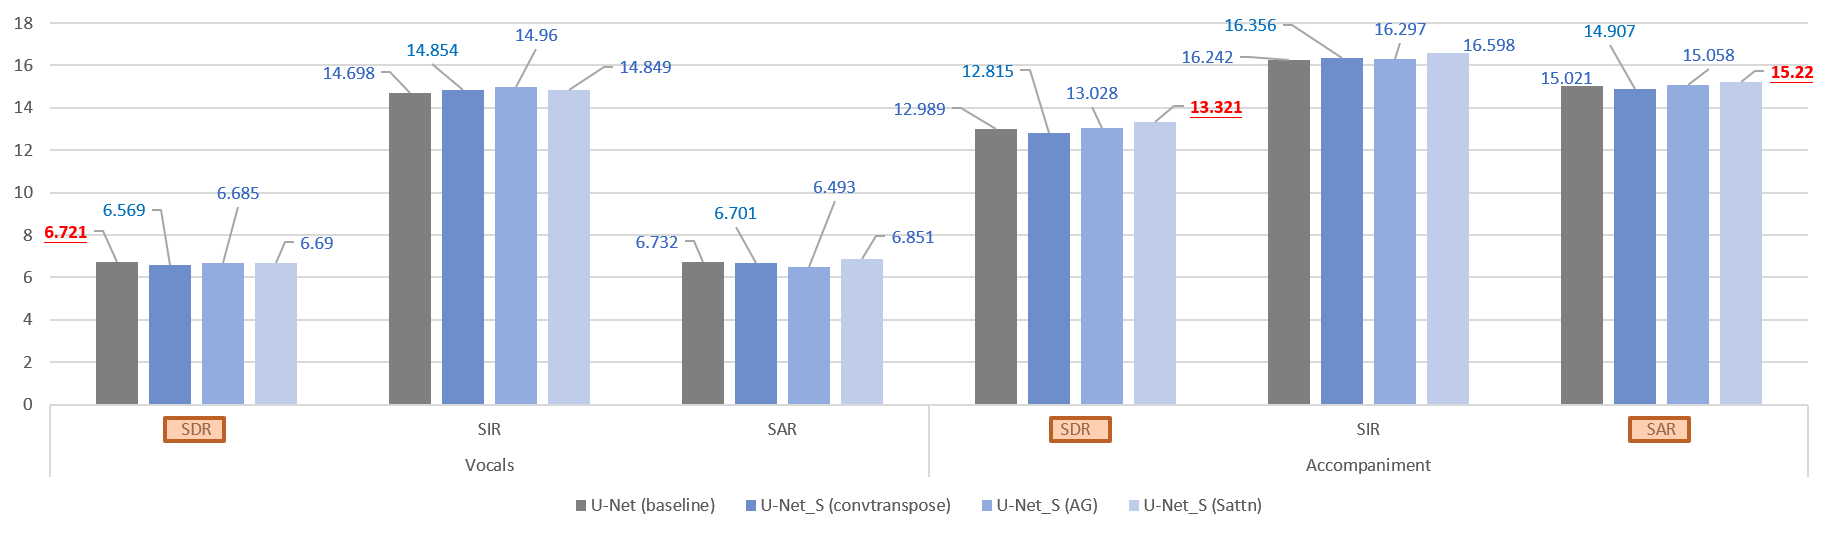
\includegraphics[width=\textwidth]{./figures/chapter05_result/attention_based_unet_result1.png}
        \caption {注意力模型的效果比較長條圖}
        \label{attention_based_unet_result1}
    \end{minipage}
    \hfil
\end{figure}

\begin{figure}[htbp]
    \hfil
    \begin{minipage}[t]{0.4\textwidth}
        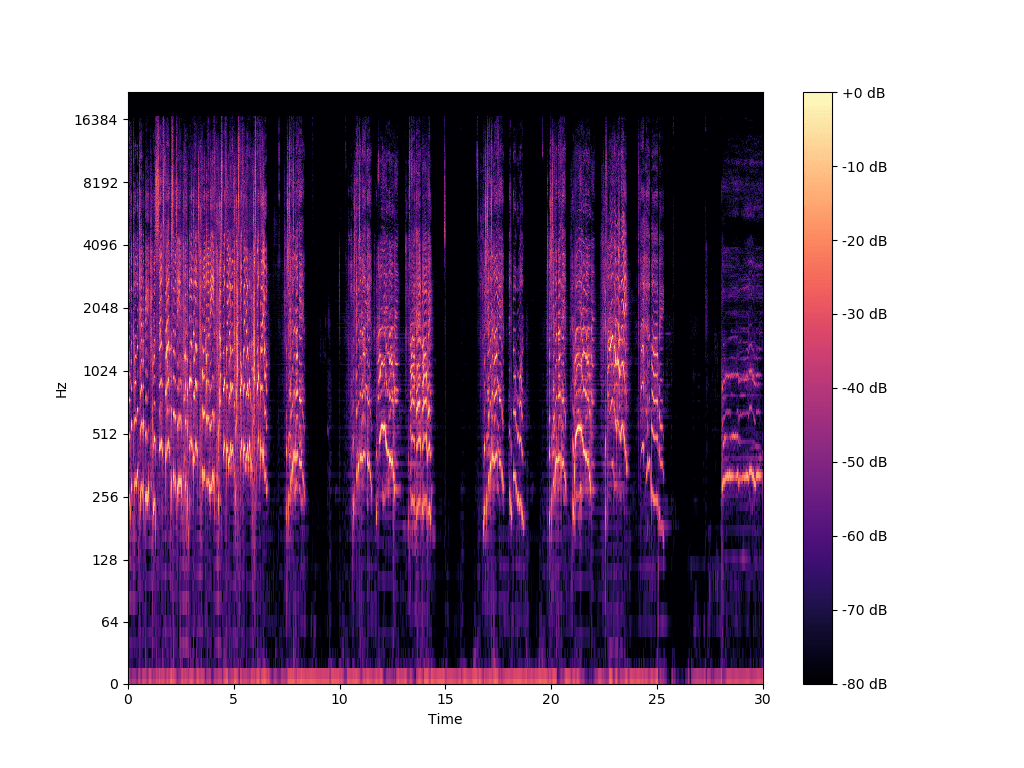
\includegraphics[width=\textwidth]{./figures/chapter05_result/6-Unet(base)_vocals.png}
        \caption {U-Net (baseline) 預測主唱音軌的頻譜圖}
        \label{U-Net6(baseline)_vocals}
    \end{minipage}
    \begin{minipage}[t]{0.4\textwidth}
        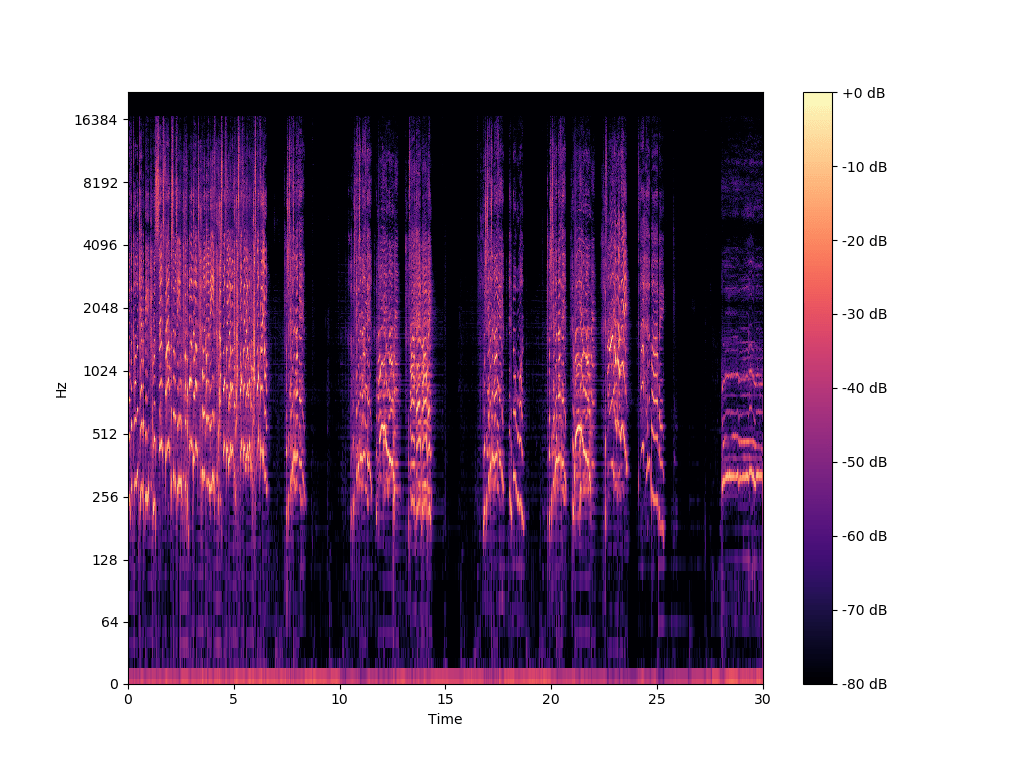
\includegraphics[width=\textwidth]{./figures/chapter05_result/6-Unet(Sattn_C-V4)_vocals.png}
        \caption {U-Net6 (Sattn) 預測主唱音軌的頻譜圖}
        \label{U-Net6(Sattn)_vocals}
    \end{minipage}
    \hfil
\end{figure}

\clearpage

\section{實驗四:模型剪枝效果比較}
模型剪枝的實驗中,表\ref{pruned_unet_table1} 記錄了 U-Net6(baseline)為基礎衍伸了兩個剪枝過後的模型,U-Net6\_s(DSConvB)與 U-Net6\_s(IRB),前者使用了深度可分卷積(Depthwise separable convolution),可以將模型大小縮為 18.71MB,後者使用 Inverted residual block 實現,可將模型大小縮為 59.8 MB。

\begin{table}[htbp]
\centering
\resizebox{\textwidth}{!}{%
\begin{tabular}{|r|c|c|l|}
\hline
 & Size (MB) & Normalization method & Note \\ \hline
U-Net6 (baseline) & 118.9 & Instance normalization &  \\ \hline
U-Net6\_s (DSConvB) & 18.71 & Batch normalization & DepthwiseSeparableConvBlock \\ \cline{1-2}
U-Net6\_s (IRB) & 59.8 &  & InvertedResidualBlock \\ \hline
\end{tabular}%
}
\caption{U-Net 的模型剪枝架構的比較}
\label{pruned_unet_table1}
\end{table}

\begin{table}[htbp]
\centering
\resizebox{\textwidth}{!}{%
\begin{tabular}{|r|l|l|l|l|}
\hline
 & Size (MB) & Up & Normalization method & Note \\ \hline
U-Net6\_s (baseline) & 118.9 & ConvT & Instance normalization & No scalability \\ \hline
U-Net6\_s (convtranspose) & 118.84 & ConvT & Instance normalization & Scalability, comparing set \\ \cline{1-4}
U-Net6\_s (upsample) & 88.08 & UpS & Instance normalization &  \\ \hline
U-Net6\_s (upsample-fusible) & 88.21 & UpS & Batch normalization & Scalability, quantization-ability \\ \hline
U-Net6\_s (DSConvB; convtranspose) & 18.71 & ConvT & Batch normalization & DepthwiseSeparableConvBlock \\ \cline{1-4}
U-Net6\_s (DSConvB; upsample) & 10.31 & UpS & Batch normalization &  \\ \hline
U-Net6\_s (IRB) & 59.8 & ConvT & Batch normalization & InvertedResidualishBlock \\ \hline
\end{tabular}%
}
\caption{模型剪枝過渡架構表}
\label{pruned_unet_table2}
\end{table}


\begin{figure}[htbp]
    \hfil
    \begin{minipage}[t]{0.45\textwidth}
        \centering
        % time series body
        \begin{tikzpicture}[scale=0.75]
        \begin{semilogyaxis} [
            xlabel = Epoch,
            ylabel = Loss,
        ]
            \addlegendentry{Training loss}
            \addplot table[mark=none, x=Step,y=Value, col sep=comma] {./numerical-data/chapter05_result/experiment04/6-Unet (base)/accompaniment/trnloss.csv};
            \addlegendentry{Validation loss}
            \addplot table[mark=none, x=Step,y=Value, col sep=comma] {./numerical-data/chapter05_result/experiment04/6-Unet (base)/accompaniment/valloss.csv};
        \end{semilogyaxis}
        \end{tikzpicture}
        % time series body
        \caption {U-Net6 (baseline) 對伴奏軌訓練的 loss}
        \label{e4:6-Unet (base):accompaniment}
    \end{minipage}
    \begin{minipage}[t]{0.45\textwidth}
        \centering
        % time series body
        \begin{tikzpicture}[scale=0.75]
        \begin{semilogyaxis} [
            xlabel = Epoch,
            ylabel = Loss,
        ]
            \addlegendentry{Training loss}
            \addplot table[mark=none, x=Step,y=Value, col sep=comma] {./numerical-data/chapter05_result/experiment04/6-Unet (base)/vocals/trnloss.csv};
            \addlegendentry{Validation loss}
            \addplot table[mark=none, x=Step,y=Value, col sep=comma] {./numerical-data/chapter05_result/experiment04/6-Unet (base)/vocals/valloss.csv};
        \end{semilogyaxis}
        \end{tikzpicture}
        % time series body
        \caption {U-Net6 (baseline) 對主唱軌訓練的 loss}
        \label{e4:6-Unet (base):vocals}
    \end{minipage}
    \hfil
\end{figure}

\begin{figure}[htbp]
    \hfil
    \begin{minipage}[t]{0.45\textwidth}
        \centering
        % time series body
        \begin{tikzpicture}[scale=0.75]
        \begin{semilogyaxis} [
            xlabel = Epoch,
            ylabel = Loss,
        ]
            \addlegendentry{Training loss}
            \addplot table[mark=none, x=Step,y=Value, col sep=comma] {./numerical-data/chapter05_result/experiment04/6-Unet (DSConvB)/accompaniment/trnloss.csv};
            \addlegendentry{Validation loss}
            \addplot table[mark=none, x=Step,y=Value, col sep=comma] {./numerical-data/chapter05_result/experiment04/6-Unet (DSConvB)/accompaniment/valloss.csv};
        \end{semilogyaxis}
        \end{tikzpicture}
        % time series body
        \caption {U-Net6\_s (DSConvB) 對伴奏軌訓練的 loss}
        \label{e4:6-Unet (DSConvB):accompaniment}
    \end{minipage}
    \begin{minipage}[t]{0.45\textwidth}
        \centering
        % time series body
        \begin{tikzpicture}[scale=0.75]
        \begin{semilogyaxis} [
            xlabel = Epoch,
            ylabel = Loss,
        ]
            \addlegendentry{Training loss}
            \addplot table[mark=none, x=Step,y=Value, col sep=comma] {./numerical-data/chapter05_result/experiment04/6-Unet (DSConvB)/vocals/trnloss.csv};
            \addlegendentry{Validation loss}
            \addplot table[mark=none, x=Step,y=Value, col sep=comma] {./numerical-data/chapter05_result/experiment04/6-Unet (DSConvB)/vocals/valloss.csv};
        \end{semilogyaxis}
        \end{tikzpicture}
        % time series body
        \caption {U-Net6\_s (DSConvB) 對主唱軌訓練的 loss}
        \label{e4:6-Unet (DSConvB):vocals}
    \end{minipage}
    \hfil
\end{figure}

\begin{figure}[htbp]
    \hfil
    \begin{minipage}[t]{0.45\textwidth}
        \centering
        % time series body
        \begin{tikzpicture}[scale=0.75]
        \begin{semilogyaxis} [
            xlabel = Epoch,
            ylabel = Loss,
        ]
            \addlegendentry{Training loss}
            \addplot table[mark=none, x=Step,y=Value, col sep=comma] {./numerical-data/chapter05_result/experiment04/6-Unet (IRB)/accompaniment/trnloss.csv};
            \addlegendentry{Validation loss}
            \addplot table[mark=none, x=Step,y=Value, col sep=comma] {./numerical-data/chapter05_result/experiment04/6-Unet (IRB)/accompaniment/valloss.csv};
        \end{semilogyaxis}
        \end{tikzpicture}
        % time series body
        \caption {U-Net6\_s (IRB) 對伴奏軌訓練的 loss}
        \label{e4:6-Unet (IRB):accompaniment}
    \end{minipage}
    \begin{minipage}[t]{0.45\textwidth}
        \centering
        % time series body
        \begin{tikzpicture}[scale=0.75]
        \begin{semilogyaxis} [
            xlabel = Epoch,
            ylabel = Loss,
        ]
            \addlegendentry{Training loss}
            \addplot table[mark=none, x=Step,y=Value, col sep=comma] {./numerical-data/chapter05_result/experiment04/6-Unet (IRB)/vocals/trnloss.csv};
            \addlegendentry{Validation loss}
            \addplot table[mark=none, x=Step,y=Value, col sep=comma] {./numerical-data/chapter05_result/experiment04/6-Unet (IRB)/vocals/valloss.csv};
        \end{semilogyaxis}
        \end{tikzpicture}
        % time series body
        \caption {U-Net6\_s (IRB) 對主唱軌訓練的 loss}
        \label{e4:6-Unet (IRB):vocals}
    \end{minipage}
    \hfil
\end{figure}


\begin{table}[htbp]
\centering
\resizebox{\textwidth}{!}{%
\begin{tabular}{|r|ccc|ccc|}
\hline
 &  & 主唱軌 &  &  & 伴奏軌 &  \\ \hline
 & \multicolumn{1}{c|}{\textbf{SDR}} & \multicolumn{1}{c|}{SIR} & SAR & \multicolumn{1}{c|}{\textbf{SDR}} & \multicolumn{1}{c|}{SIR} & \textbf{SAR} \\ \hline
\textit{U-Net6 (baseline)} & \multicolumn{1}{c|}{\textit{6.721}} & \multicolumn{1}{c|}{\textit{14.698}} & \textit{6.732} & \multicolumn{1}{c|}{\textit{12.989}} & \multicolumn{1}{c|}{\textit{16.242}} & \textit{15.021} \\ \hline
U-Net6\_s (DSConvB; convtranspose) & \multicolumn{1}{c|}{5.981} & \multicolumn{1}{c|}{14.169} & 6.044 & \multicolumn{1}{c|}{12.308} & \multicolumn{1}{c|}{16.016} & 14.143 \\ \hline
U-Net\_s (IRB) & \multicolumn{1}{c|}{\textbf{6.51}} & \multicolumn{1}{c|}{13.989} & 6.486 & \multicolumn{1}{c|}{\textbf{12.771}} & \multicolumn{1}{c|}{15.985} & \textbf{14.769} \\ \hline
\end{tabular}%
}
\caption{模型剪枝的效果比較表}
\label{pruned_unet_table3}
\end{table}

\begin{figure}[htbp]
    \hfil
    \begin{minipage}[t]{1.0\textwidth}
        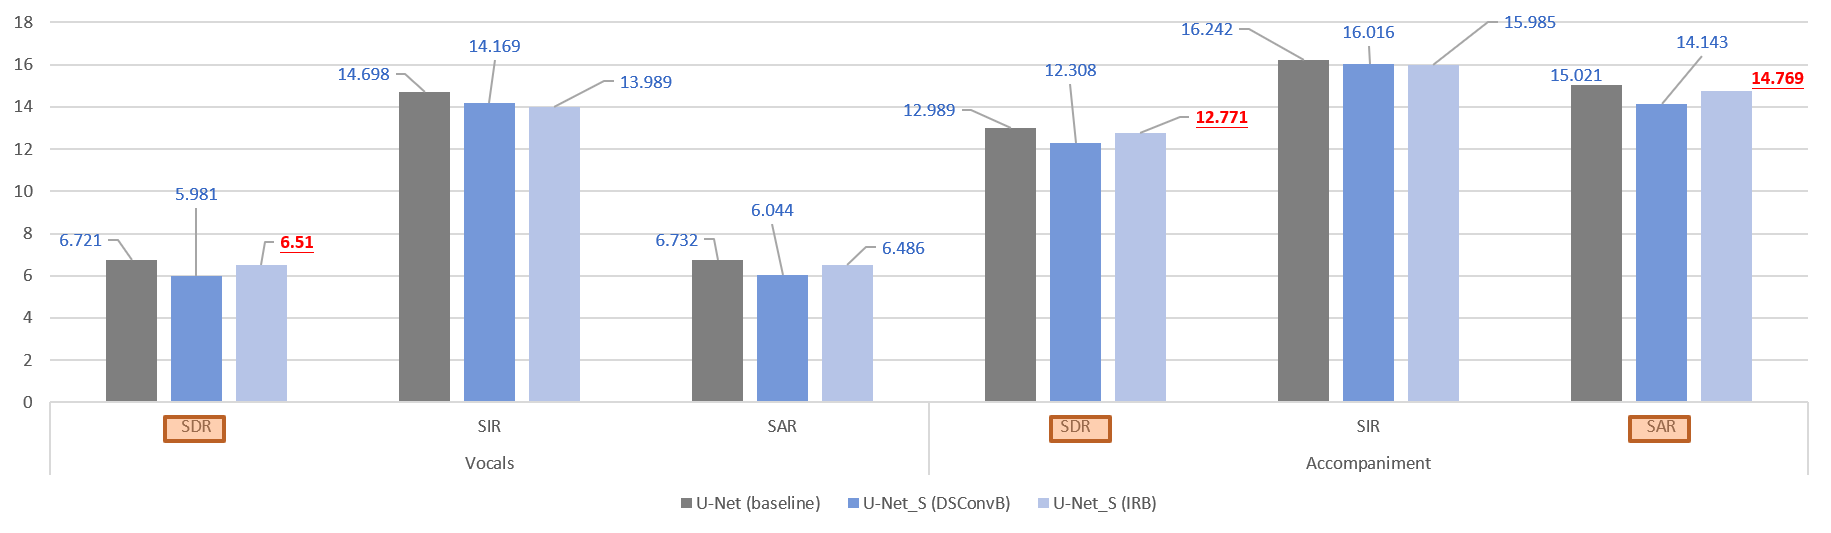
\includegraphics[width=\textwidth]{./figures/chapter05_result/pruned_unet_result1.png}
        \caption {模型剪枝的效果比較長條圖}
        \label{pruned_unet_result1}
    \end{minipage}
    \hfil
\end{figure}

\clearpage

\section{實驗五:模型量化效果比較}
% 量化結果有時間的話應仍要在完整的 Musdb18 中測試其 metrics
量化實驗中,要從所有的候選模型中挑選(表\ref{quantization_table1} 與表 \ref{quantization_table2} ),本實驗選擇三個模型做量化,分別是:U-Net6\_s(upsample)、U-Net6\_s(DSConvB; convtranspose)與 U-Net6\_s (IRB),並使用 QNNPACK~\cite{dukhan2018qnnpack,wu2019machine} 實現。U-Net6\_s(upsample) 是模型量化實驗中,用來  評估基準模型量化過後的能力,為 U-Net6(baseline) 的微調版本。選擇 U-Net6\_s(DSConvB; convtranspose)的原因是模型參數最少,而使用 convtranspose 的狀態又比使用 upsample 時還要好,固選之。選擇 U-Net6 (IRB) 是因為其模型參數量介於中間,用來作為比較使用。

以下模型:U-Net6\_s(upsample)(表\ref{quantization_table3}與圖\ref{quantization_result1})、U-Net6\_s(DSConvB; convtranspose)(表\ref{quantization_table4}與圖\ref{quantization_result2})與 U-Net6 (IRB)(表\ref{quantization_table5}與圖\ref{quantization_result3})。以訓練的模型再使用 Musdb18 的七秒資料集中做「校準」,最後使用該資料及與 museval 測試量化後的效果。Musdb18 的七秒資料集是官方將原本資料集的每首歌做裁減,縮小該資料集,在本實驗中的校準階段需要大量的時間,以該資料集可不失歌曲種類的多樣性,但也可很好得量化模型。

\begin{table}[htbp]
\centering
\resizebox{\textwidth}{!}{%
\begin{tabular}{|r|c|c|c|l|}
\hline
 & Size (MB) & Up & Normalization method & Note \\ \hline
U-Net6 (baseline) & 118.9 & ConvT & Instance normalization & No scalability \\ \hline
U-Net6\_s (convtranspose) & 118.84 & ConvT & Instance normalization & Scalability, comparing set \\ \cline{1-4}
U-Net6\_s (upsample) & 88.08 & UpS & Instance normalization &  \\ \hline
U-Net6\_s (upsample-fusible) & 88.21 & UpS & Batch normalization & Scalability, quantization-ability \\ \hline
\textbf{U-Net6\_s (DSConvB; convtranspose)} & \textbf{18.71} & ConvT & Batch normalization & DepthwiseSeparableConvBlock \\ \cline{1-4}
U-Net6\_s (DSConv; upsample) & 10.31 & UpS & Batch normalization &  \\ \hline
\textbf{U-Net6\_s (IRB)} & \textbf{59.8} & ConvT & Batch normalization & InvertedResidualishBlock \\ \hline
\end{tabular}%
}
\caption{模型量化的候選表}
\label{quantization_table1}
\end{table}

\begin{table}[htbp]
\centering
\resizebox{\textwidth}{!}{%
\begin{tabular}{|r|ccc|ccc|}
\hline
 &  & 主唱軌 &  &  & 伴奏軌 &  \\ \hline
 & \multicolumn{1}{c|}{\textbf{SDR}} & \multicolumn{1}{c|}{SIR} & SAR & \multicolumn{1}{c|}{\textbf{SDR}} & \multicolumn{1}{c|}{SIR} & \textbf{SAR} \\ \hline
\textit{U-Net6 (baseline)} & \multicolumn{1}{c|}{\textit{6.721}} & \multicolumn{1}{c|}{\textit{14.698}} & \textit{6.732} & \multicolumn{1}{c|}{\textit{12.989}} & \multicolumn{1}{c|}{\textit{16.242}} & \textit{15.021} \\ \hline
U-Net6\_s (convtranspose) & \multicolumn{1}{c|}{6.569} & \multicolumn{1}{c|}{14.854} & 6.701 & \multicolumn{1}{c|}{12.815} & \multicolumn{1}{c|}{16.356} & 14.907 \\ \hline
U-Net6\_s (upsample) & \multicolumn{1}{c|}{6.553} & \multicolumn{1}{c|}{13.986} & 6.383 & \multicolumn{1}{c|}{13.013} & \multicolumn{1}{c|}{16.412} & 14.746 \\ \hline
U-Net6\_s (upsample-fusible) & \multicolumn{1}{c|}{6.612} & \multicolumn{1}{c|}{14.66} & 6.845 & \multicolumn{1}{c|}{12.918} & \multicolumn{1}{c|}{16.226} & 14.932 \\ \hline
\textbf{U-Net6 (DSConvB; convtranspose)} & \multicolumn{1}{c|}{5.981} & \multicolumn{1}{c|}{14.169} & 6.044 & \multicolumn{1}{c|}{12.308} & \multicolumn{1}{c|}{16.016} & 14.143 \\ \hline
U-Net6 (DSConvB; upsample) & \multicolumn{1}{c|}{5.922} & \multicolumn{1}{c|}{13.925} & 5.929 & \multicolumn{1}{c|}{12.278} & \multicolumn{1}{c|}{15.653} & 14.325 \\ \hline
\textbf{U-Net6 (IRB)} & \multicolumn{1}{c|}{6.51} & \multicolumn{1}{c|}{13.989} & 6.486 & \multicolumn{1}{c|}{12.771} & \multicolumn{1}{c|}{15.985} & 14.769 \\ \hline
\end{tabular}%
}
\caption{模型量化候選模型的效果表}
\label{quantization_table2}
\end{table}

\begin{table}[htbp]
\centering
\resizebox{\textwidth}{!}{%
\begin{tabular}{|r|ccc|ccc|}
\hline
 &  & 主唱軌 &  &  & 伴奏軌 &  \\ \hline
 & \multicolumn{1}{c|}{\textbf{SDR}} & \multicolumn{1}{c|}{SIR} & SAR & \multicolumn{1}{c|}{\textbf{SDR}} & \multicolumn{1}{c|}{SIR} & \textbf{SAR} \\ \hline
\textit{U-Net6\_s (upsample-fusible)} & \multicolumn{1}{c|}{\textit{7.275}} & \multicolumn{1}{c|}{\textit{11.228}} & \textit{8.259} & \multicolumn{1}{c|}{\textit{12.17}} & \multicolumn{1}{c|}{\textit{14.795}} & \textit{15.057} \\ \hline
Default quantization & \multicolumn{1}{c|}{6.919} & \multicolumn{1}{c|}{11.374} & 8.115 & \multicolumn{1}{c|}{\textbf{11.813}} & \multicolumn{1}{c|}{14.254} & 14.569 \\ \hline
Advance quantization & \multicolumn{1}{c|}{\textbf{7.160}} & \multicolumn{1}{c|}{11.082} & 8.096 & \multicolumn{1}{c|}{11.551} & \multicolumn{1}{c|}{13.848} & \textbf{14.866} \\ \hline
\end{tabular}%
}
\caption{U-Net6\_s(upsample-fusible)量化效果表}
Model size: 88.21 (MB) vs. 22.09 (MB)
\label{quantization_table3}
\end{table}


\begin{figure}[htbp]
    \hfil
    \begin{minipage}[t]{1.0\textwidth}
        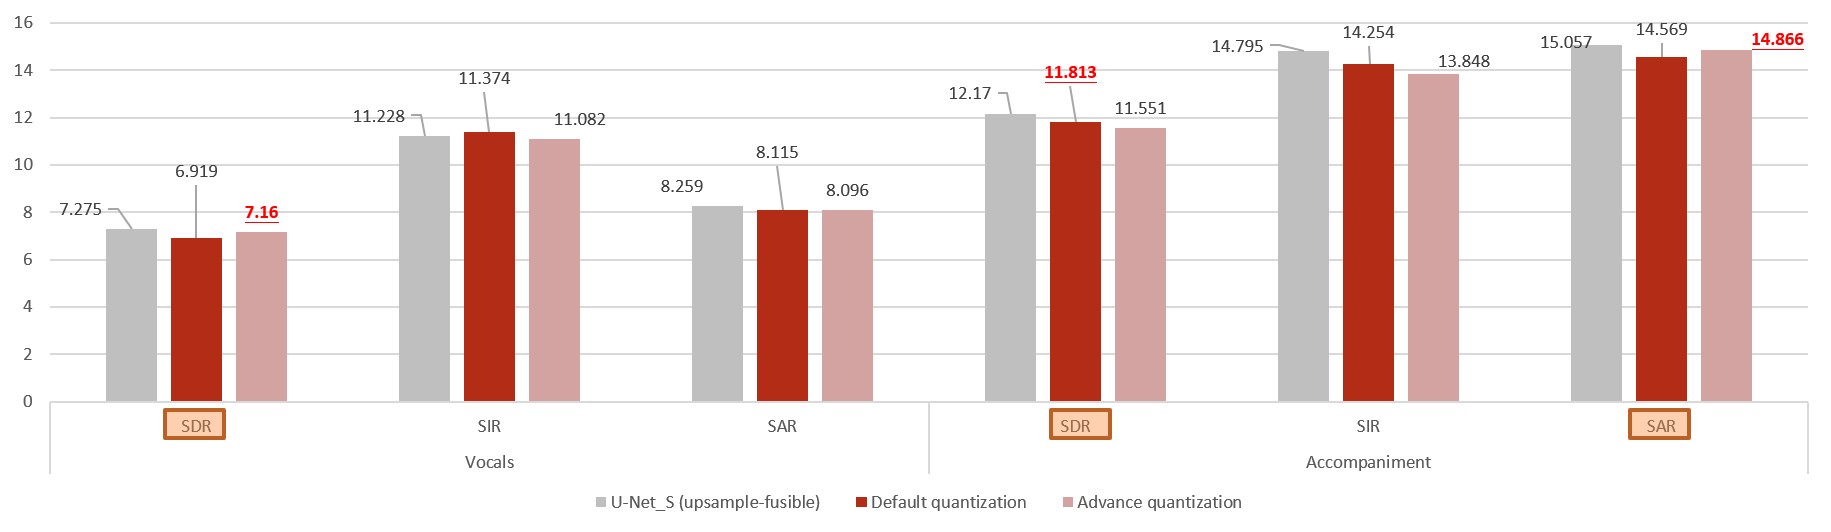
\includegraphics[width=\textwidth]{./figures/chapter05_result/quantization_result1.png}
        \caption {U-Net6\_s(upsample-fusible)量化效果長條圖}
        \label{quantization_result1}
    \end{minipage}
    \hfil
\end{figure}


\begin{table}[htbp]
\centering
\resizebox{\textwidth}{!}{%
\begin{tabular}{|r|ccc|ccc|}
\hline
 &  & 主唱軌 &  &  & 伴奏軌 &  \\ \hline
 & \multicolumn{1}{c|}{\textbf{SDR}} & \multicolumn{1}{c|}{SIR} & SAR & \multicolumn{1}{c|}{\textbf{SDR}} & \multicolumn{1}{c|}{SIR} & \textbf{SAR} \\ \hline
\textit{U-Net6\_s (DSConvB; convtranspose)} & \multicolumn{1}{c|}{\textit{6.648}} & \multicolumn{1}{c|}{\textit{11.019}} & \textit{7.471} & \multicolumn{1}{c|}{\textit{11.428}} & \multicolumn{1}{c|}{\textit{14.54}} & \textit{14.171} \\ \hline
Default quantization & \multicolumn{1}{c|}{3.028} & \multicolumn{1}{c|}{11.214} & 7.143 & \multicolumn{1}{c|}{\textbf{11.184}} & \multicolumn{1}{c|}{14.92} & \textbf{13.993} \\ \hline
Advance quantization & \multicolumn{1}{c|}{\textbf{5.87}} & \multicolumn{1}{c|}{10.424} & 7.306 & \multicolumn{1}{c|}{11.041} & \multicolumn{1}{c|}{14.357} & 13.655 \\ \hline
\end{tabular}%
}
\caption{U-Net6\_s(DSConvB; convtranspose)量化效果表}
Model size: 18.71 (MB) vs. 4.75 (MB)
\label{quantization_table4}
\end{table}

\begin{figure}[htbp]
    \hfil
    \begin{minipage}[t]{1.0\textwidth}
        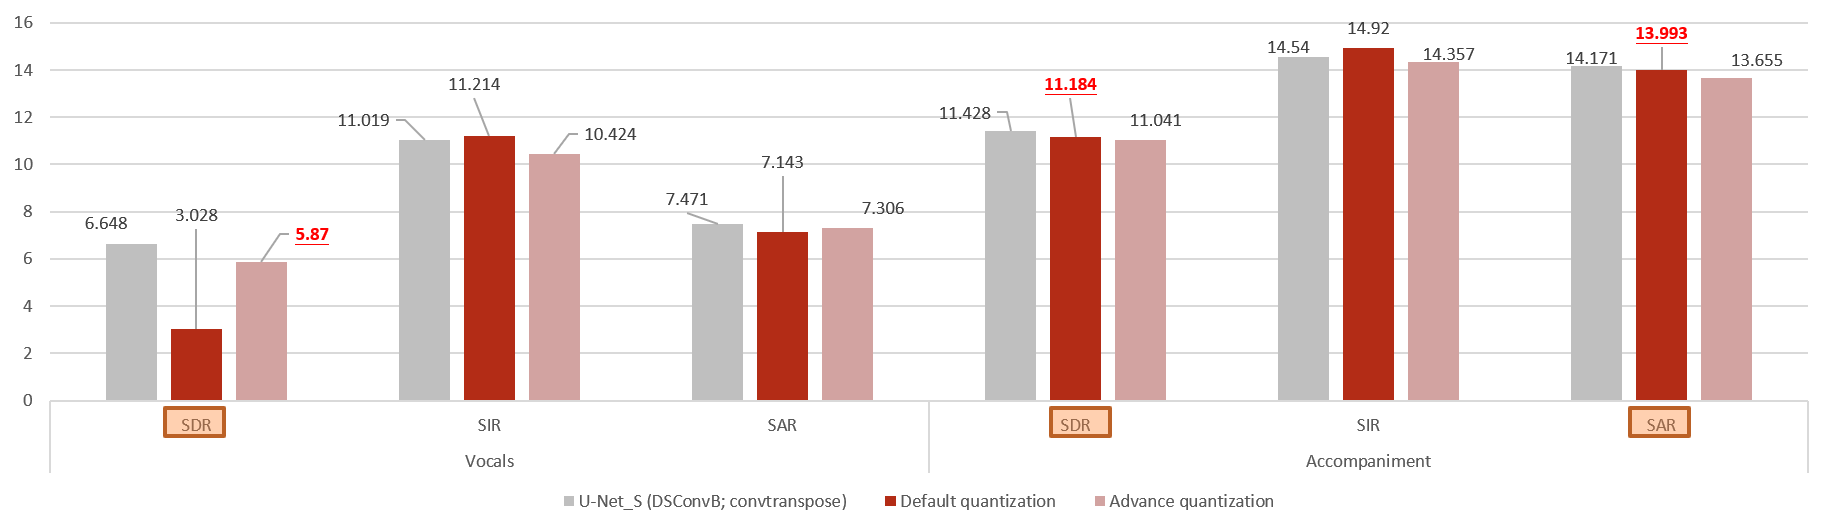
\includegraphics[width=\textwidth]{./figures/chapter05_result/quantization_result2.png}
        \caption {U-Net6\_s(DSConvB; convtranspose)量化效果長條圖}
        \label{quantization_result2}
    \end{minipage}
    \hfil
\end{figure}

\begin{table}[htbp]
\centering
\resizebox{\textwidth}{!}{%
\begin{tabular}{|r|ccc|ccc|}
\hline
 &  & 主唱軌 &  &  & 伴奏軌 &  \\ \hline
 & \multicolumn{1}{c|}{\textbf{SDR}} & \multicolumn{1}{c|}{SIR} & SAR & \multicolumn{1}{c|}{\textbf{SDR}} & \multicolumn{1}{c|}{SIR} & \textbf{SAR} \\ \hline
\textit{U-Net6\_s (IRB)} & \multicolumn{1}{c|}{\textit{6.691}} & \multicolumn{1}{c|}{\textit{10.75}} & \textit{8.166} & \multicolumn{1}{c|}{\textit{11.816}} & \multicolumn{1}{c|}{\textit{14.829}} & \textit{15.021} \\ \hline
Default quantization & \multicolumn{1}{c|}{\textbf{6.446}} & \multicolumn{1}{c|}{10.345} & 7.895 & \multicolumn{1}{c|}{6.009} & \multicolumn{1}{c|}{14.799} & 8.969 \\ \hline
Advance quantization & \multicolumn{1}{c|}{6.362} & \multicolumn{1}{c|}{10.361} & 7.728 & \multicolumn{1}{c|}{\textbf{11.048}} & \multicolumn{1}{c|}{15.059} & \textbf{13.6} \\ \hline
\end{tabular}%
}
\caption{U-Net6\_s (IRB) 量化效果表}
Model size: 59.80 (MB) vs. 15.07 (MB)
\label{quantization_table5}
\end{table}

\begin{figure}[htbp]
    \hfil
    \begin{minipage}[t]{1.0\textwidth}
        \includegraphics[width=\textwidth]{./figures/chapter05_result/quantization_result3.png}
        \caption {U-Net6\_s (IRB) 量化效果長條圖}
        \label{quantization_result3}
    \end{minipage}
    \hfil
\end{figure}
\chapter{結論與未來展望}


\section{結論}

由上章所有實驗的效果可以歸結出下列結論:
\begin{itemize}
    \item[1.] 實驗一的結果可以知道,直接使用 U-Net 輸出的頻譜與混音軌的相位直接合併輸出,會導致相位無法對應,進而導致輸出的音訊效果。但若使用輸出的所有頻譜作出 ratio mask filter 或是 Wiener filter,直接對混音軌的 STFT 做濾波,可以避免相位無法對應的問題,也可以確保輸出的音量可以與原本一致,整體效果有大幅度的增進。
    \item[2.] 實驗二的結果可以知道,對 U-Net 輸出的頻譜做頻譜刪減法,可有小幅度的增進效能,降低主唱軌與伴奏軌相互干擾的問題。
    \item[3.] 實驗三的實驗可以知道,U-Net 模型在長片段的聲音中,不易找到相同聲音模式的聲音,但加上注意力機制後,可以明顯地將殘留在主唱預測音軌的鼓聲去除。
    \item[4.] 深度可分卷積與 Inverted residual 可以有效地縮小 U-Net 模型,剪枝過後的模型仍保有聲音分離的能力,但後者能力稍強,可以針對應用場域的需求做出調整。
    \item[5.] 模型皆可以有效的量化,代表此模型能在手機端或是筆電端皆有機會可以應用,甚至可在實時的場域中作使用。
\end{itemize}


\section{未來展望}

U-Net在聲音訊號分離仍有很多值得了解的面向。注意力模型 attention gate~\cite{oktay2018attention} 方法其中的 $\alpha$ 值目前為給定狀態,未來可測試不同參數,或是讓機器可以自主學習。針對模型剪枝方法(深度可分卷積~\cite{chollet2017xception,howard2017mobilenets}與 inverted residual~\cite{sandler2018mobilenetv2})導致的效果下滑,可對其再加上注意力機制 self-attention~\cite{shaw2018self} 或是 attention gate~\cite{oktay2018attention} 進行實驗。

上面談到是對模型改善的方法,另外可對其訓練資料—頻譜圖下手,比如 spleeter~\cite{hennequin2020spleeter} 就想讓模型專注在人耳比較敏感的區域訓練即可,其在模型中以變數 F 做調整,在最後的版本選擇以 1024 個 frequency bin 頻譜圖輸入至 U-Net 中訓練,這是在人耳敏感度、模型專注度與模型預測時間各方的妥協下所產生,這也可應用在本論文探討的 U-Net 之下,越小的輸入可以讓模型預測時間更快,實時應用的緩衝更小。再者,liu~\cite{liu2020channel} 提到的「Channel-wise Subband Input」也是基於此理論,在不同的頻段中,使用不同的模型架構對症下藥,不只可以縮小模型所需的參數,也可讓模型專注在各自的頻段上讓效果更好,也值得在本論文架構上做進一步探討。

本論文基於的 U-Net 架構上有一個短版,也就是無法利用聲音訊號中的相位資訊,這也是 Demucs~\cite{defossez2019music} 所想要克服的問題,其用到了 LSTM~\cite{gers1999learning} 對時間序列的資訊取得做優化,但可能導致運算量增加或是運算時間無法因卷積的優勢降低,對此 Giri~\cite{giri2019attention} 提出的「Attention wave-u-net」可以解決此問題,將 LSTM 以 attention 替換值得在未來的實驗中探討。或是在 STFT 域中,繼續使用二維卷積的 U-Net 訓練,對此,Choi 等人~\cite{choi2018phase} 提出的「Phase-aware speech enhancement with deep complex u-net」值得研究,直接使用 STFT 之後的值,而非單取其 Magnitude 成為模型的輸入,讓模型學習相位的變化。

% 在 loss 函數上也可有很多著墨點
不只針對 U-Net 上的優化,loss 函數也是一個值得研究的方向。一個好的 loss 函數幫助整個深度神經網路,在本論文中的所有模型採用 SmoothL1Loss 函數,但是否能使用這邊採取的評估指標 SDR、SIR 與 SAR 作為 loss 函數?Nakajima~\cite{nakajima2018monaural} 等人提出了可能性,其將深度神經網路的輸出以 SDR 計算其與正確的訊號之間的 loss,在最後的評估時也取得了更好的成績。另外,Braun~\cite{braun2020consolidated} 等人與 gusó 的碩士論文~\cite{guso2020on_loss_functions} 針對語音強化(speech enhancement)與音樂分離領域做了一個完整的討論,將所有可以在監督式學習的 loss 函數列出,在未來可參考此研究,找到本架構最適合的 loss 函數。

% 頻譜刪減法在 nn 上實現
% 其他模型在 svs 上的應用可能
頻譜刪減法的討論,可參考在 Rohman~\cite{rohman2016novel} 等人的研究。還有非 U-Net 架構在音樂分離領域上的可能性,Tzinis~\cite{tzinis2020improving} 等人提出利用聲音辨別系統幫助聲音分離架構,Samuel~\cite{samuel2020meta} 等人提出利用 Meta-learning 方法幫助聲音分離架構。

% slakh2100 資料集以擴充各個樂器的資料
在資料的處理上面,為了之後其他樂器音軌的分離,需要拓展現有的資料,slakh2100~\cite{manilow2019cutting} 裡有需多高品質混音的樂器聲音,還有如何對資料做 augmentation 可以參考 Uhlich~\cite{uhlich2017improving} 等人的研究。

在模型預測能力與時間需求上,與其他模型來做比較如下圖。其中圖\ref{pic_conclusions1} 是代表訓練過程中,對於一秒的聲音,大約需要多少時間。圖\ref{pic_conclusions2} 是代表一秒的聲音分離時,加上檔案讀寫的時間,平均需要多少時間。由此可見,雖然 Spleeter 使用的 frquency-based 模型的分離速度的確很快,比起 Demucs 使用的 time-based 模型快很多,雖然本研究也是使用 frequency-based 模型,分離效果不錯但在速度上太過緩慢。未來研究中,調控 encoder 與 decoder 的層數,在效能與速度上取得平衡。

\begin{figure}[htbp]
    \hfil
    \begin{minipage}[t]{0.60\textwidth}
        \includegraphics[width=\textwidth]{./figures/chapter06_conclusions/pic_conclusions1.png}
        \caption {一秒聲音需訓練的時間}
        \label{pic_conclusions1}
    \end{minipage}
    \hfil
\end{figure}

\begin{figure}[htbp]
    \hfil
    \begin{minipage}[t]{0.60\textwidth}
        \includegraphics[width=\textwidth]{./figures/chapter06_conclusions/pic_conclusions2.png}
        \caption {一秒聲音平均分離的時間}
        \label{pic_conclusions2}
    \end{minipage}
    \hfil
\end{figure}

% 參考文獻
% References
\refmatter
\bibliographystyle{abbrv}
\bibliography{back/references}

% 附錄
% Appendices
% !TeX root = ../main.tex

\appendix{A}{提出模型的完整訓練}


\section{U-Net6 (Sattn) 的 L1 loss 下降趨勢}

\begin{figure}[htbp]
    \hfil
    \begin{minipage}[t]{0.45\textwidth}
        \centering
        % time series body
        \begin{tikzpicture}[scale=0.75]
        \begin{semilogyaxis} [
            xlabel = Epoch,
            ylabel = Loss,
        ]
            \addlegendentry{Training loss}
            \addplot table[mark=none, x=Step,y=Value, col sep=comma] {./numerical-data/chapter05_result/experiment-extra/6-Unet (Sattn_C-V4)/vocals/trnloss.csv};
            \addlegendentry{Validation loss}
            \addplot table[mark=none, x=Step,y=Value, col sep=comma] {./numerical-data/chapter05_result/experiment-extra/6-Unet (Sattn_C-V4)/vocals/valloss.csv};
        \end{semilogyaxis}
        \end{tikzpicture}
        % time series body
        \caption {U-Net6 (Sattn) 對主唱軌訓練的 loss 趨勢圖}
        \label{a:6-Unet (Self-attntion):vocals}
    \end{minipage}
    \begin{minipage}[t]{0.45\textwidth}
        \centering
        % time series body
        \begin{tikzpicture}[scale=0.75]
        \begin{semilogyaxis} [
            xlabel = Epoch,
            ylabel = Loss,
        ]
            \addlegendentry{Training loss}
            \addplot table[mark=none, x=Step,y=Value, col sep=comma] {./numerical-data/chapter05_result/experiment-extra/6-Unet (Sattn_C-V4)/accompaniment/trnloss.csv};
            \addlegendentry{Validation loss}
            \addplot table[mark=none, x=Step,y=Value, col sep=comma] {./numerical-data/chapter05_result/experiment-extra/6-Unet (Sattn_C-V4)/accompaniment/valloss.csv};
        \end{semilogyaxis}
        \end{tikzpicture}
        % time series body
        \caption {U-Net6 (Sattn) 對伴奏軌訓練的 loss 趨勢圖}
        \label{a:6-Unet (Self-attntion):accompaniment}
    \end{minipage}
    \hfil
\end{figure}

\section{U-Net6 (DSConB) 的 L1 loss 下降趨勢}

\begin{figure}[htbp]
    \hfil
    \begin{minipage}[t]{0.45\textwidth}
        \centering
        % time series body
        \begin{tikzpicture}[scale=0.75]
        \begin{semilogyaxis} [
            xlabel = Epoch,
            ylabel = Loss,
        ]
            \addlegendentry{Training loss}
            \addplot table[mark=none, x=Step,y=Value, col sep=comma] {./numerical-data/chapter05_result/experiment-extra/6-Unet (DSConvB)/vocals/trnloss.csv};
            \addlegendentry{Validation loss}
            \addplot table[mark=none, x=Step,y=Value, col sep=comma] {./numerical-data/chapter05_result/experiment-extra/6-Unet (DSConvB)/vocals/valloss.csv};
        \end{semilogyaxis}
        \end{tikzpicture}
        % time series body
        \caption {U-Net6 (DSConvB) 對主唱軌訓練的 loss 趨勢圖}
        \label{a:6-Unet (DSConvB):vocals}
    \end{minipage}
    \begin{minipage}[t]{0.45\textwidth}
        \centering
        % time series body
        \begin{tikzpicture}[scale=0.75]
        \begin{semilogyaxis} [
            xlabel = Epoch,
            ylabel = Loss,
        ]
            \addlegendentry{Training loss}
            \addplot table[mark=none, x=Step,y=Value, col sep=comma] {./numerical-data/chapter05_result/experiment-extra/6-Unet (DSConvB)/accompaniment/trnloss.csv};
            \addlegendentry{Validation loss}
            \addplot table[mark=none, x=Step,y=Value, col sep=comma] {./numerical-data/chapter05_result/experiment-extra/6-Unet (DSConvB)/accompaniment/valloss.csv};
        \end{semilogyaxis}
        \end{tikzpicture}
        % time series body
        \caption {U-Net6 (DSConvB) 對伴奏軌訓練的 loss 趨勢圖}
        \label{a:6-Unet (DSConvB):accompaniment}
    \end{minipage}
    \hfil
\end{figure}

\section{U-Net6 (IRB) 的 L1 loss 下降趨勢}

\begin{figure}[htbp]
    \hfil
    \begin{minipage}[t]{0.45\textwidth}
        \centering
        % time series body
        \begin{tikzpicture}[scale=0.75]
        \begin{semilogyaxis} [
            xlabel = Epoch,
            ylabel = Loss,
        ]
            \addlegendentry{Training loss}
            \addplot table[mark=none, x=Step,y=Value, col sep=comma] {./numerical-data/chapter05_result/experiment-extra/6-Unet (IRB)/vocals/trnloss.csv};
            \addlegendentry{Validation loss}
            \addplot table[mark=none, x=Step,y=Value, col sep=comma] {./numerical-data/chapter05_result/experiment-extra/6-Unet (IRB)/vocals/valloss.csv};
        \end{semilogyaxis}
        \end{tikzpicture}
        % time series body
        \caption {U-Net6 (IRB) 對主唱軌訓練的 loss 趨勢圖}
        \label{a:6-Unet (IRB):vocals}
    \end{minipage}
    \begin{minipage}[t]{0.45\textwidth}
        \centering
        % time series body
        \begin{tikzpicture}[scale=0.75]
        \begin{semilogyaxis} [
            xlabel = Epoch,
            ylabel = Loss,
        ]
            \addlegendentry{Training loss}
            \addplot table[mark=none, x=Step,y=Value, col sep=comma] {./numerical-data/chapter05_result/experiment-extra/6-Unet (IRB)/accompaniment/trnloss.csv};
            \addlegendentry{Validation loss}
            \addplot table[mark=none, x=Step,y=Value, col sep=comma] {./numerical-data/chapter05_result/experiment-extra/6-Unet (IRB)/accompaniment/valloss.csv};
        \end{semilogyaxis}
        \end{tikzpicture}
        % time series body
        \caption {U-Net6 (IRB) 對伴奏軌訓練的 loss 趨勢圖}
        \label{a:6-Unet (IRB):accompaniment}
    \end{minipage}
    \hfil
\end{figure}

\section{以 Museval 指標與目前技術比較}

資料來源:
\begin{itemize}
    \item \url{https://github.com/facebookresearch/demucs} (FB: Demucs, Tasnet)
    \item \url{https://github.com/deezer/spleeter} (Deezer: Spleeter)
    \item \url{https://github.com/f90/Wave-U-Net} (Wave-u-net)
    \item \url{https://github.com/sigsep/sigsep-mus-2018} (Sony: MMDenseLSTM, MMDenseNet)
\end{itemize}

\begin{table}[htbp]
\centering
\resizebox{\linewidth}{!}{
\begin{tabular}{|r|c|c|c|c|}
\hline
\multicolumn{1}{|l|}{} & \multicolumn{3}{c|}{主唱軌} & Note \\ \hline
\multicolumn{1}{|l|}{} & \textbf{SDR} & SIR & SAR &  \\ \hline
\textit{U-Net6 (baseline) w/o filter} & \textit{7.269} & \textit{15.045} & \textit{7.224} & \textit{baseline, extra data} \\ \hline
\textbf{U-Net6 (baseline) w/ wiener} & 7.648 & 18.593 & 7.436 & \textbf{proposed, extra data} \\ \hline
\textbf{U-Net6 (Sattn) w/ wiener} & \textbf{7.800} & 18.977 & 7.750 & \textbf{proposed, extra data} \\ \hline
\textbf{U-Net6\_s (DSConvB) w/ wiener} & 6.780 & 18.525 & 6.314 & \textbf{proposed, extra data} \\ \hline
\textbf{U-Net6\_s (IRB) w/ ratio mask} & 4.702 & 16.81 & 3.996 & \textbf{proposed, extra data} \\ \hline
FB: Demucs & 6.721 & 11.704 & 1.740 & extra data \\ \hline
FB: Tasnet & 6.618 & 12.038 & 2.143 & extra data \\ \hline
Deezer: Spleeter (2-stem) & 6.361 & 17.362 & 5.679 & extra data \\ \hline
Wave-u-net (for SVS) & 4.971 & 13.988 & 4.408 & only on musdb18 \\ \hline
Sony: MMDenseLSTM & 7.159 & 16.485 & 7.484 & extra data \\ \hline
Sony: MMDenseNet & 6.799 & 15.366 & 7.035 & extra data \\ \hline
\end{tabular}
}
\caption{與先進音樂人聲分離模型比較(主唱軌)}
\label{tab:proposed-and-other_vocals}
\end{table}

\begin{table}[htbp]
\centering
\resizebox{\linewidth}{!}{
\begin{tabular}{|r|c|c|c|c|}
\hline
\multicolumn{1}{|l|}{} & \multicolumn{3}{c|}{伴奏軌} & Note \\ \hline
\multicolumn{1}{|l|}{} & \textbf{SDR} & SIR & \textbf{SAR} &  \\ \hline
\textit{U-Net6 (baseline) w/o filter} & \textit{13.805} & \textit{16.785} & \textit{14.52} & \textit{baseline, extra data} \\ \hline
\textbf{U-Net6 (baseline) w/ wiener} & 14.288 & 20.332 & 14.815 & \textbf{proposed, extra data} \\ \hline
\textbf{U-Net6 (Sattn) w/ wiener} & \textbf{14.457} & 20.412 & \textbf{15.114} & \textbf{proposed, extra data} \\ \hline
\textbf{U-Net6\_s (DSConvB) w/ wiener} & 13.520 & 18.680 & 14.202 & \textbf{proposed, extra data} \\ \hline
\textbf{U-Net6\_s (IRB) w/ ratio mask} & 11.200 & 14.567 & 13.056 & \textbf{proposed, extra data} \\ \hline
FB: Demucs & 13.441 & 9.334 & 7.014 & extra data \\ \hline
FB: Tasnet & 12.695 & 11.087 & 7.168 & extra data \\ \hline
Deezer: Spleeter (2-stem) & 12.510 & 18.201 & 12.911 & extra data \\ \hline
Wave-u-net (for SVS) & 11.106 & 15.302 & 11.439 & only on musdb18 \\ \hline
Sony: MMDenseLSTM & 13.737 & 18.499 & 14.583 & extra data \\ \hline
Sony: MMDenseNet & 13.290 & 18.418 & 14.350 & extra data \\ \hline
\end{tabular}
}
\caption{與先進音樂人聲分離模型比較(伴奏軌)}
\label{tab:proposed-and-other_accompaniment}
\end{table}

\clearpage

\section{有無使用 Musdb18 資料集訓練之差異}

\begin{table}[htbp]
\centering
\begin{tabular}{|r|c|c|}
\hline
 & 主唱軌 SDR & 伴奏軌 SDR \\ \hline
U-Net6 (baseline) & 6.953 & 13.403 \\ \hline
U-Net6 (baseline, extra) & 7.648 & 14.288 \\ \hline
U-Net6 (Sattn) & 7.133 & 13.714 \\ \hline
U-Net6 (Sattn, extra) & 7.8 & 14.457 \\ \hline
U-Net6 (AG) & 7.097 & 13.526 \\ \hline
U-Net6 (AG, extra) & 7.437 & 14.121 \\ \hline
Demucs (extra) & 7.29 & 13.441 \\ \hline
Spleeter (extra w/o musdb18) & 6.86 & 12.51 \\ \hline
\end{tabular}
\caption{使用額外資料訓練在 SDR 上的差異}
\label{tab:whether_additional_data}
\end{table}

\end{document}
